\chapter{PENGUJIAN DAN ANALISIS}
\label{chap:pengujiananalisis}

\section{Alat dan Bahan}
\label{sec:alatdanbahan}

\subsection{Perangkat Pelatihan Model \emph{Machine Learning}}

Pelatihan model dilakukan pada perangkat komputer dengan spesifikasi sebagai berikut:

\begin{table}[htbp]
  \centering
  \begin{tabular}{|l|l|}
  \hline
  \textbf{Prosesor} & Intel® Core™ i5-1235U \\
  \hline
  \textbf{GPU} & NVIDIA Geforce MX550 GDDR6 (2GB VRAM) \\
  \hline
  \textbf{RAM} & 16GB DDR4 \\
  \hline
  \textbf{Penyimpanan} & 512GB SSD M.2 PCIe \\
  \hline
  \textbf{Sistem Operasi} & Linux Ubuntu 22.04 Jammy Jellyfish \\
  \hline
  \textbf{Framework} & Tensorflow 2.15 \& PyTorch 2.3.0 \\
  \hline
  \textbf{Lingkungan Pengembangan} & Python 3.10.12 \\
  \hline
  \end{tabular}
  \caption{Spesifikasi perangkat \emph{laptop} untuk pelatihan model}
  \label{tab:training_laptop_specs}
\end{table}
Model yang digunakan adalah SSD MobileNetV2 yang dilatih menggunakan dataset kendaraan hasil anotasi sendiri dan milik dari penelitian Prismadika Yuniar \parencite*{prismadika2023}. Proses pelatihan dilakukan selama 30 dan 50 \emph{epoch} dengan batch size 16, learning rate 0.01, dan \emph{scheduler} antara CosineAnnealingLR dan MultiStepLR. Dataset terdiri dari masing-masing 165 dan 200 gambar kendaraan sebelum augmentasi, yang dibagi menjadi data latih (80\%) dan data validasi (20\%).

\subsection{\emph{Edge Device} untuk \emph{Inference}}

Untuk menjalankan sistem deteksi secara real-time, model hasil pelatihan dikonversi dari format PyTorch Tensor (.pt) ke ONNX (.onnx) dengan tujuan untuk diimplementasikan pada perangkat edge. Pengujian dilakukan pada perangkat \emph{edge} yang memiliki spesifikasi sebagai berikut:

\subsubsection{Perangkat 1: NVIDIA Jetson Nano 4GB}

Perangkat pertama yang digunakan adalah NVIDIA Jetson Nano 4GB yang merupakan sistem berbasis ARM yang dirancang untuk aplikasi edge computing dengan kemampuan grafis yang optimal. Jetson Nano memiliki GPU Maxwell dengan 128 CUDA cores yang memungkinkan pemrosesan model deep learning secara efisien. Kamera yang digunakan pada pengujian ini adalah Logitech C920 HD Pro USB Webcam yang dapat memberikan kualitas video 1080p pada 30 FPS, cukup untuk pengolahan deteksi kendaraan secara real-time. Tabel \ref{tab:jetson_nano_specs} menunjukkan spesifikasi perangkat Jetson Nano yang digunakan dalam penelitian ini.

\begin{table}[htbp]
  \centering
  \begin{tabular}{|l|l|}
  \hline
  \textbf{Perangkat} & NVIDIA Jetson Nano 4GB \\
  \hline
  \textbf{CPU} & Quad-core ARM Cortex-A57 MPCore processor \\
  \hline
  \textbf{GPU} & NVIDIA Maxwell 128 NVIDIA CUDA® cores \\
  \hline
  \textbf{RAM} & 4 GB 64-bit LPDDR4, 1600MHz 25.6 GB/s \\
  \hline
  \textbf{Penyimpanan} & 16 GB eMMC 5.1 \\
  \hline
  \textbf{Sistem Operasi} & Linux Ubuntu 18.04 Bionic Beaver \\
  \hline
  \textbf{Kamera} & Logitech C920 HD Pro USB Webcam \\
  \hline
  \textbf{Lingkungan Pengembangan} & Python 3.6.9 \\
  \hline
  \end{tabular}
  \caption{Spesifikasi perangkat \emph{edge} pertama untuk \emph{inference}}
  \label{tab:jetson_nano_specs}
\end{table}

\subsubsection{Perangkat 2: Beelink Gemini T34}

Selain menggunakan Jetson Nano, perangkat kedua yang digunakan dalam pengujian adalah Beelink Gemini T34, sebuah mini PC dengan kemampuan komputasi yang cukup untuk aplikasi deteksi real-time. Beelink Gemini T34 dilengkapi dengan prosesor Intel Celeron dan GPU Intel HD Graphics 600, yang mendukung akselerasi inferensi untuk model deep learning. Perangkat ini cocok untuk pengolahan data video dan real-time inferencing, sehingga memudahkan implementasi model pada sistem gerbang tol. Tabel \ref{tab:beelink_t34_specs} menunjukkan spesifikasi perangkat Beelink Gemini T34 yang digunakan dalam penelitian ini.

\begin{table}[htbp]
  \centering
  \begin{tabular}{|l|l|}
  \hline
  \textbf{Perangkat} & Beelink Gemini T34 \\
  \hline
  \textbf{CPU} & Intel Celeron N3450 Quad-core \\
  \hline
  \textbf{GPU} & Intel HD Graphics 500 \\
  \hline
  \textbf{RAM} & 8 GB DDR3L \\
  \hline
  \textbf{Penyimpanan} & 256 GB SSD M.2 SATA \\
  \hline
  \textbf{Sistem Operasi} & Linux Ubuntu 20.04 Focal Fossa \\
  \hline
  \textbf{Kamera} & Logitech C920 HD Pro USB Webcam \\
  \hline
  \textbf{Lingkungan Pengembangan} & Python 3.8.10 \\
  \hline
  \end{tabular}
  \caption{Spesifikasi perangkat \emph{edge} kedua untuk \emph{inference}}
  \label{tab:beelink_t34_specs}
\end{table}

Dengan penggunaan dua perangkat ini, yaitu NVIDIA Jetson Nano yang lebih fokus pada aplikasi edge dengan akselerasi GPU untuk deep learning, serta Beelink Gemini T34 yang menawarkan solusi berbasis prosesor Intel untuk komputasi ringan, pengujian dilakukan untuk melihat perbandingan performa dan kecocokan setiap perangkat untuk aplikasi deteksi kendaraan overdimensi secara real-time.

\subsection{Spesifikasi \emph{Server Cloud}}

Untuk mendukung pengolahan backend dan pengelolaan data dari perangkat edge, sistem ini menggunakan \emph{Virtual Private Server} (VPS) yang dihosting di cloud. VPS ini digunakan untuk menjalankan layanan backend seperti manajemen database, penyimpanan data kendaraan yang terdeteksi, serta komunikasi antara perangkat edge dan server cloud. Berikut adalah spesifikasi VPS yang digunakan:

\begin{table}[htbp]
  \centering
  \begin{tabular}{|l|l|}
  \hline
  \textbf{Provider} & Biznet Gio \\
  \hline
  \textbf{Tipe VPS} & Neo Lite \\
  \hline
  \textbf{CPU} & 1 vCPU (Intel Xeon) \\
  \hline
  \textbf{RAM} & 2 GB \\
  \hline
  \textbf{Penyimpanan} & 60 GB SSD \\
  \hline
  \textbf{Sistem Operasi} & Ubuntu 22.04 LTS \\
  \hline
  \textbf{IP Address} & Static Public IP \\
  \hline
  \textbf{Lingkungan Pengembangan} & Node.js v20.19.1  \\
  \hline
  \end{tabular}
  \caption{Spesifikasi Server Cloud untuk Hosting Backend}
  \label{tab:cloud_server_specs}
  \end{table}

\subsection{Lingkungan Pengujian}

Lingkungan pengujian alat dilakukan di Gerbang Tol Dupak 2, Genting Kalianak, Asem Rowo, Surabaya, Jawa Timur. Pengujian dilakukan pada hari Senin, 28 April 2025, Kamis 1 Mei 2025, dan Jumat 2 Mei 2025. Masing-masing hari pengujian dilakukan pada pukul 08:00 - 12:00 WIB. 

Perangkat kamera ditempatkan pada ketinggian ... meter dari permukaan jalan dengan sudut kemiringan 45 derajat ke arah lajur kendaraan. Posisi ini dipilih untuk memastikan penangkapan gambar yang optimal dari bagian depan kendaraan yang melintasi gerbang tol. Jarak pengambilan gambar dari perangkat kamera ke objek kendaraan ... meter.

Lalu lintas kendaraan selama pengujian tercatat rata-rata 120-150 kendaraan per jam dengan variasi jenis kendaraan meliputi mobil penumpang (55\%), truk ringan (25\%), truk sedang (15\%), dan kendaraan berat (5\%). Perangkat edge ditempatkan di pinggir gerbang tol dengan koneksi internet berkecepatan 3-5 Mbps menggunakan hostpot dari handphone untuk transmisi data ke server cloud. Gambar \ref{fig:testing_environment} menunjukkan setup perangkat pada lokasi pengujian.

% Tambahkan gambar setup pengujian
\begin{figure}[htbp]
  \centering
  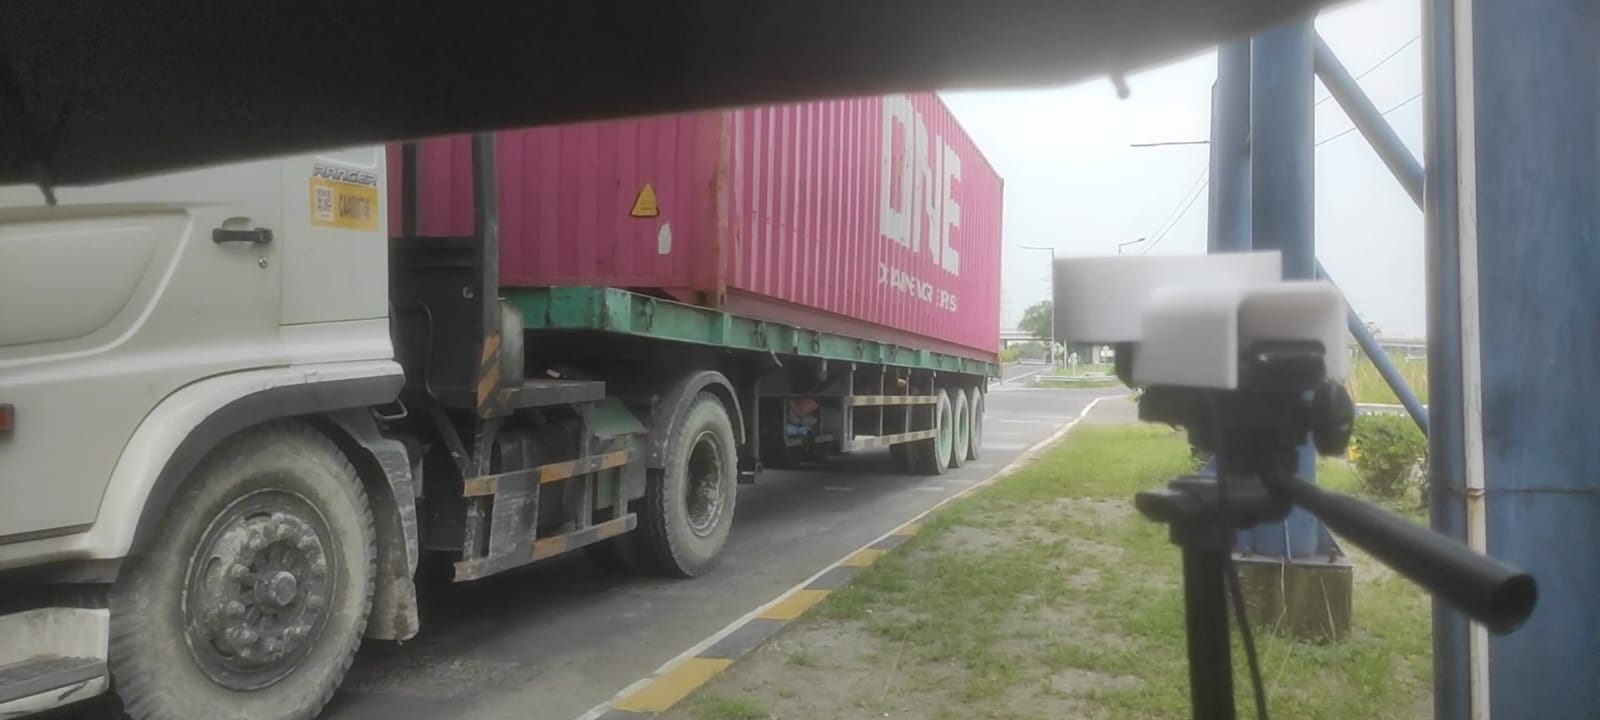
\includegraphics[width=0.8\textwidth]{gambar/bab4-test-dupak-kamera.jpeg}
  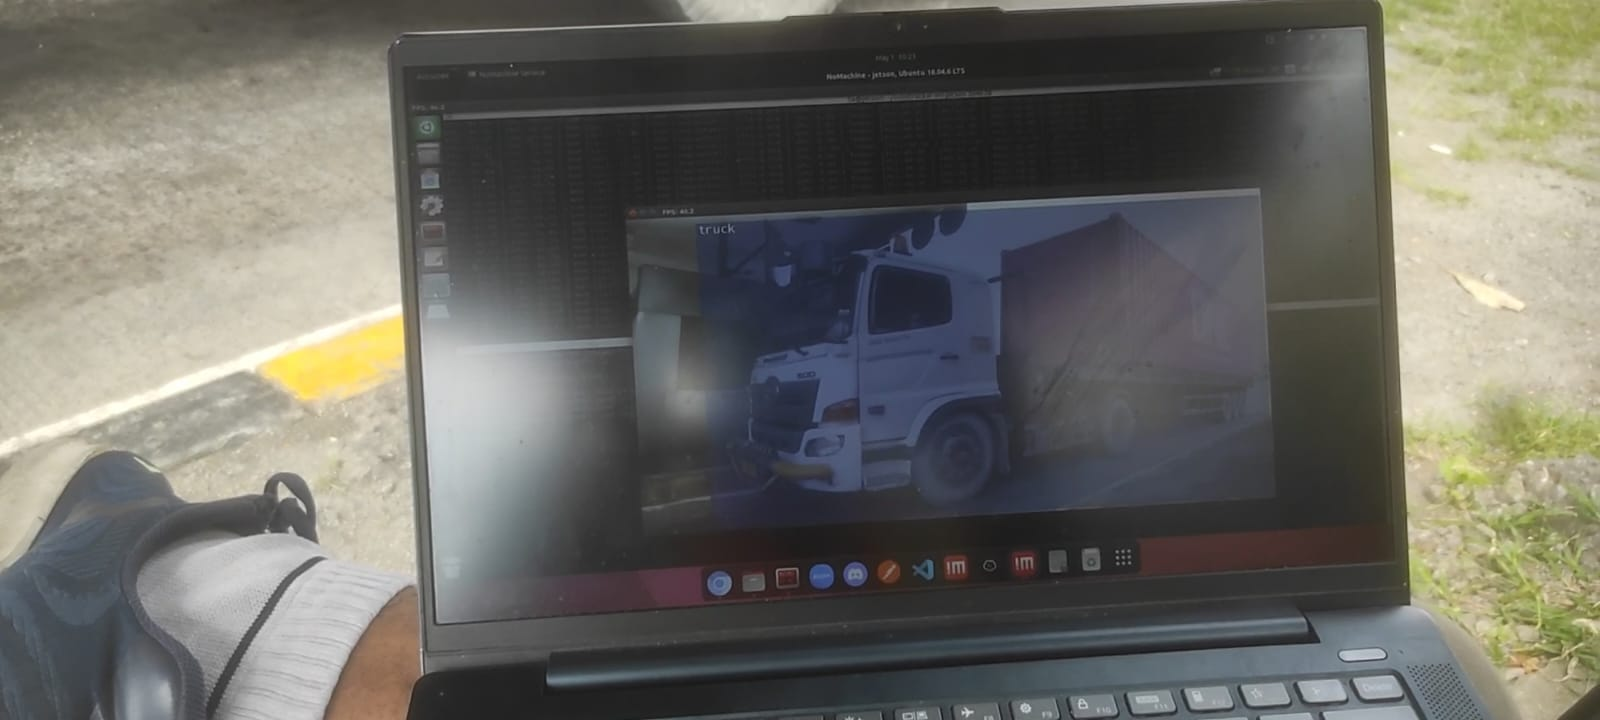
\includegraphics[width=0.8\textwidth]{gambar/bab4-test-dupak-monitor.jpeg}
  \caption{Setup perangkat pada lokasi pengujian di Gerbang Tol Dupak 2}
  \label{fig:testing_environment}
\end{figure}

\section{Model SSD-MobileNetV2}
\label{sec:model_ssd_mobilenetv2}

\subsection{Analisis Hasil Latih Model}

Hasil pelatihan model SSD-MobileNetV2 pada dataset kendaraan dianalisis berdasarkan beberapa metrik evaluasi yang umum digunakan dalam deteksi objek. Model dilatih dengan konfigurasi 16 batch size, learning rate 0.01, dan 4 konfigurasi berbeda, yaitu:

\begin{itemize}[nolistsep]
  \item 30 \emph{epoch} dan \emph{scheduler} CosineAnnealingLR
  \item 30 \emph{epoch} dan \emph{scheduler} MultiStepLR
  \item 50 \emph{epoch} dan \emph{scheduler} CosineAnnealingLR
  \item 50 \emph{epoch} dan \emph{scheduler} MultiStepLR
\end{itemize}\

Selama proses pelatihan, berbagai metrik dipantau untuk menganalisis konvergensi model, meliputi \emph{accuracy}, \emph{precision}, \emph{recall}, \emph{F1 score}, \emph{regression loss}, \emph{classification loss}, dan \emph{total loss}. Grafik di bawah ini menunjukkan hasil pelatihan untuk masing-masing konfigurasi.

\begin{figure}[htbp]
  \centering
  \begin{subfigure}{0.45\textwidth}
    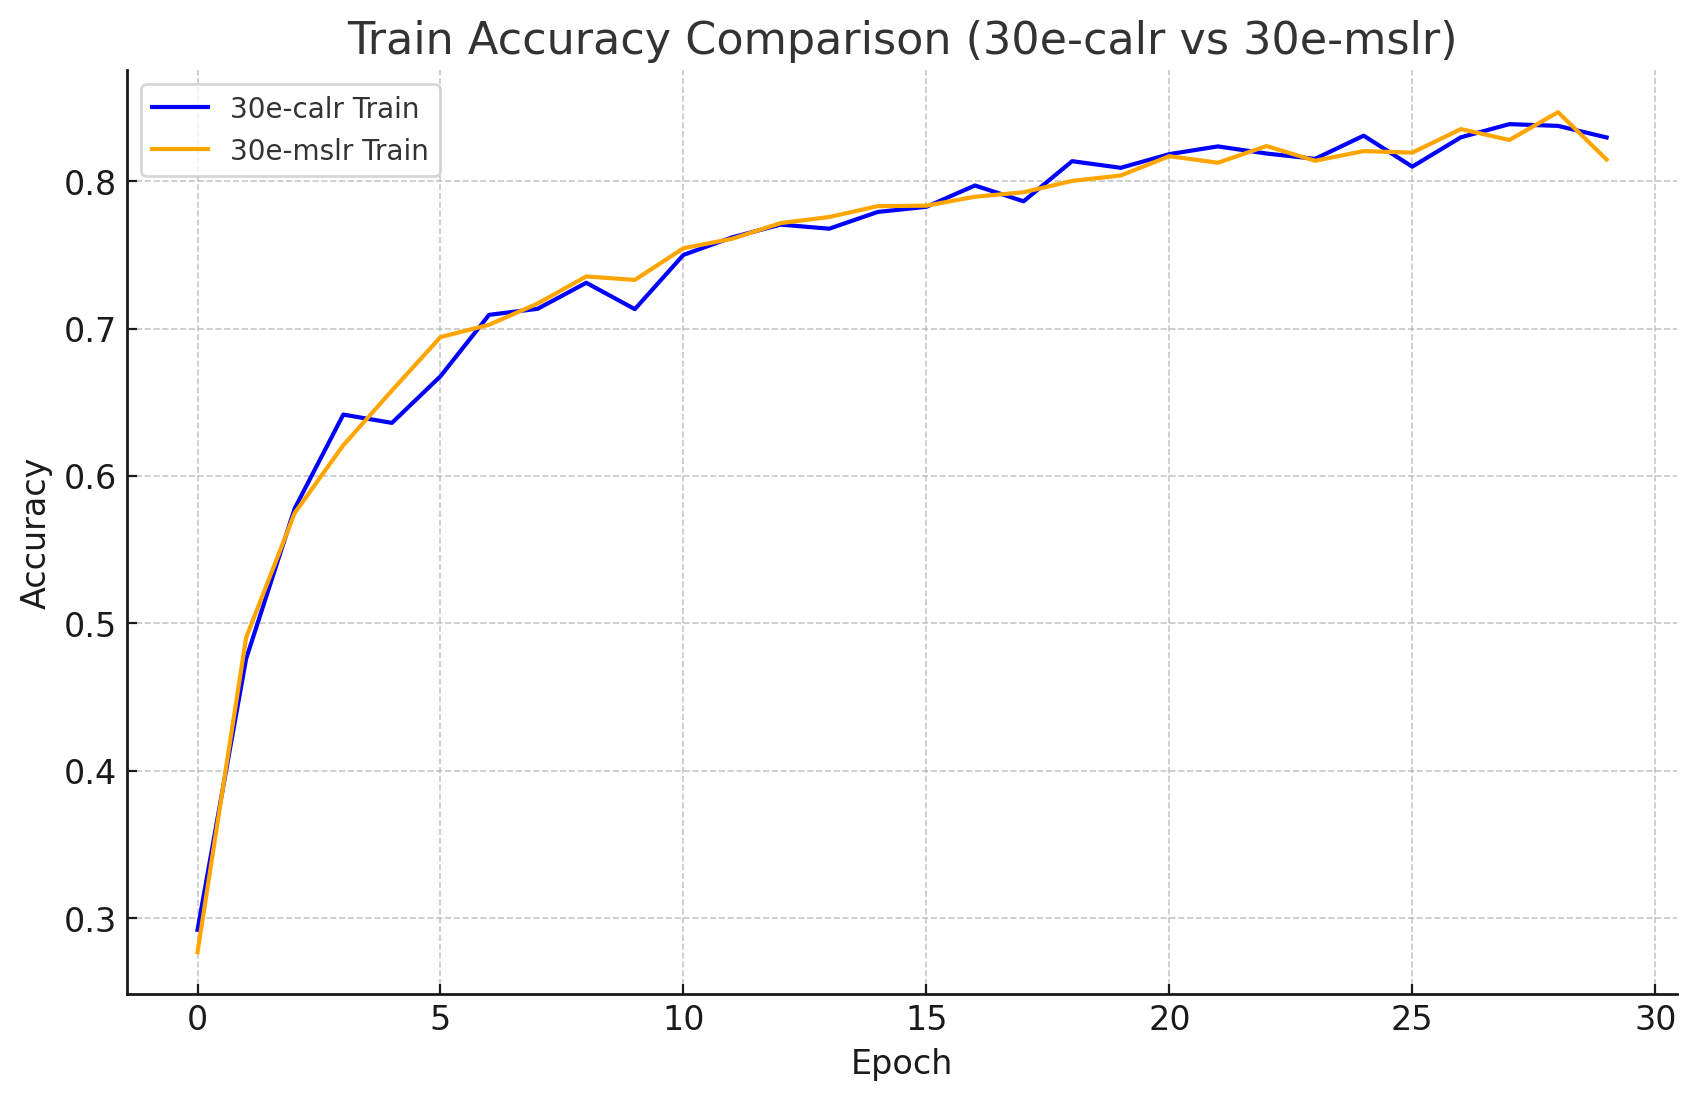
\includegraphics[width=\textwidth]{gambar/bab4-train-acc-30e.png}
    \caption{Accuracy (training) - 30 \emph{epoch}}
  \end{subfigure}
  \hfill
  \begin{subfigure}{0.45\textwidth}
    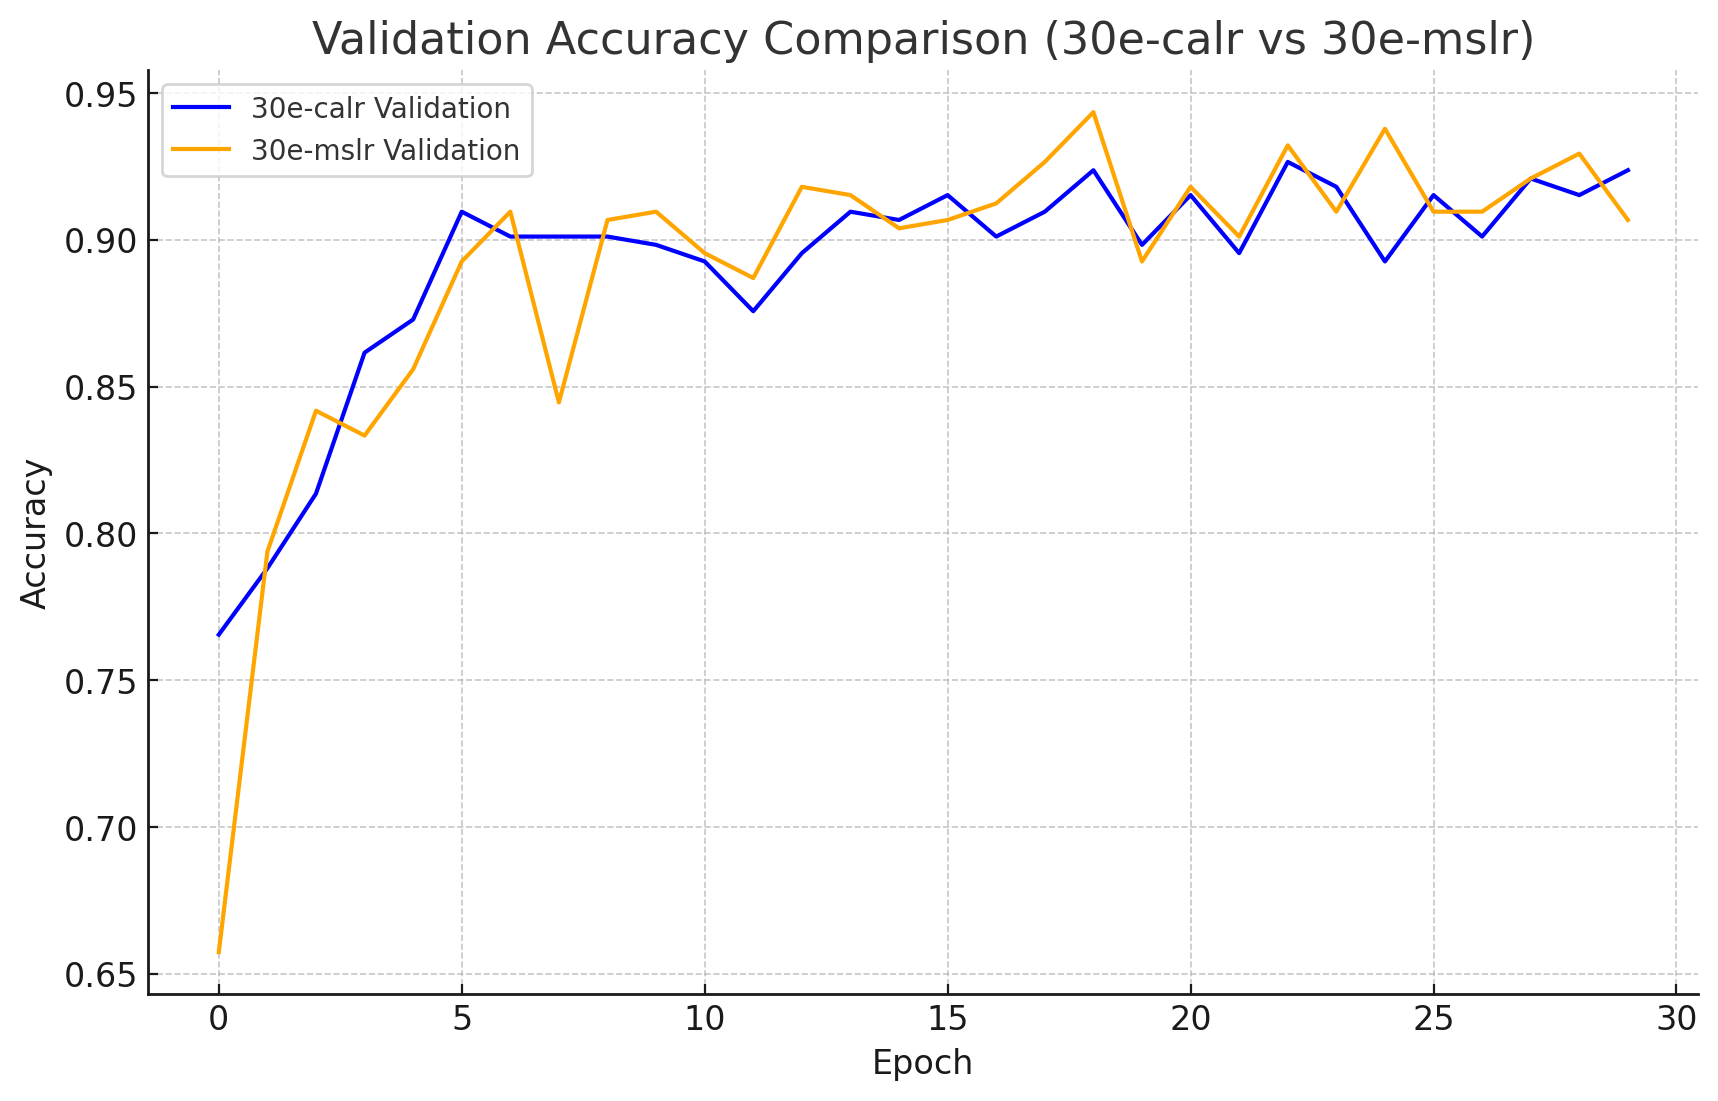
\includegraphics[width=\textwidth]{gambar/bab4-val-acc-30e.png}
    \caption{Accuracy (validation) - 30 \emph{epoch}}
  \end{subfigure}
  \begin{subfigure}{0.45\textwidth}
    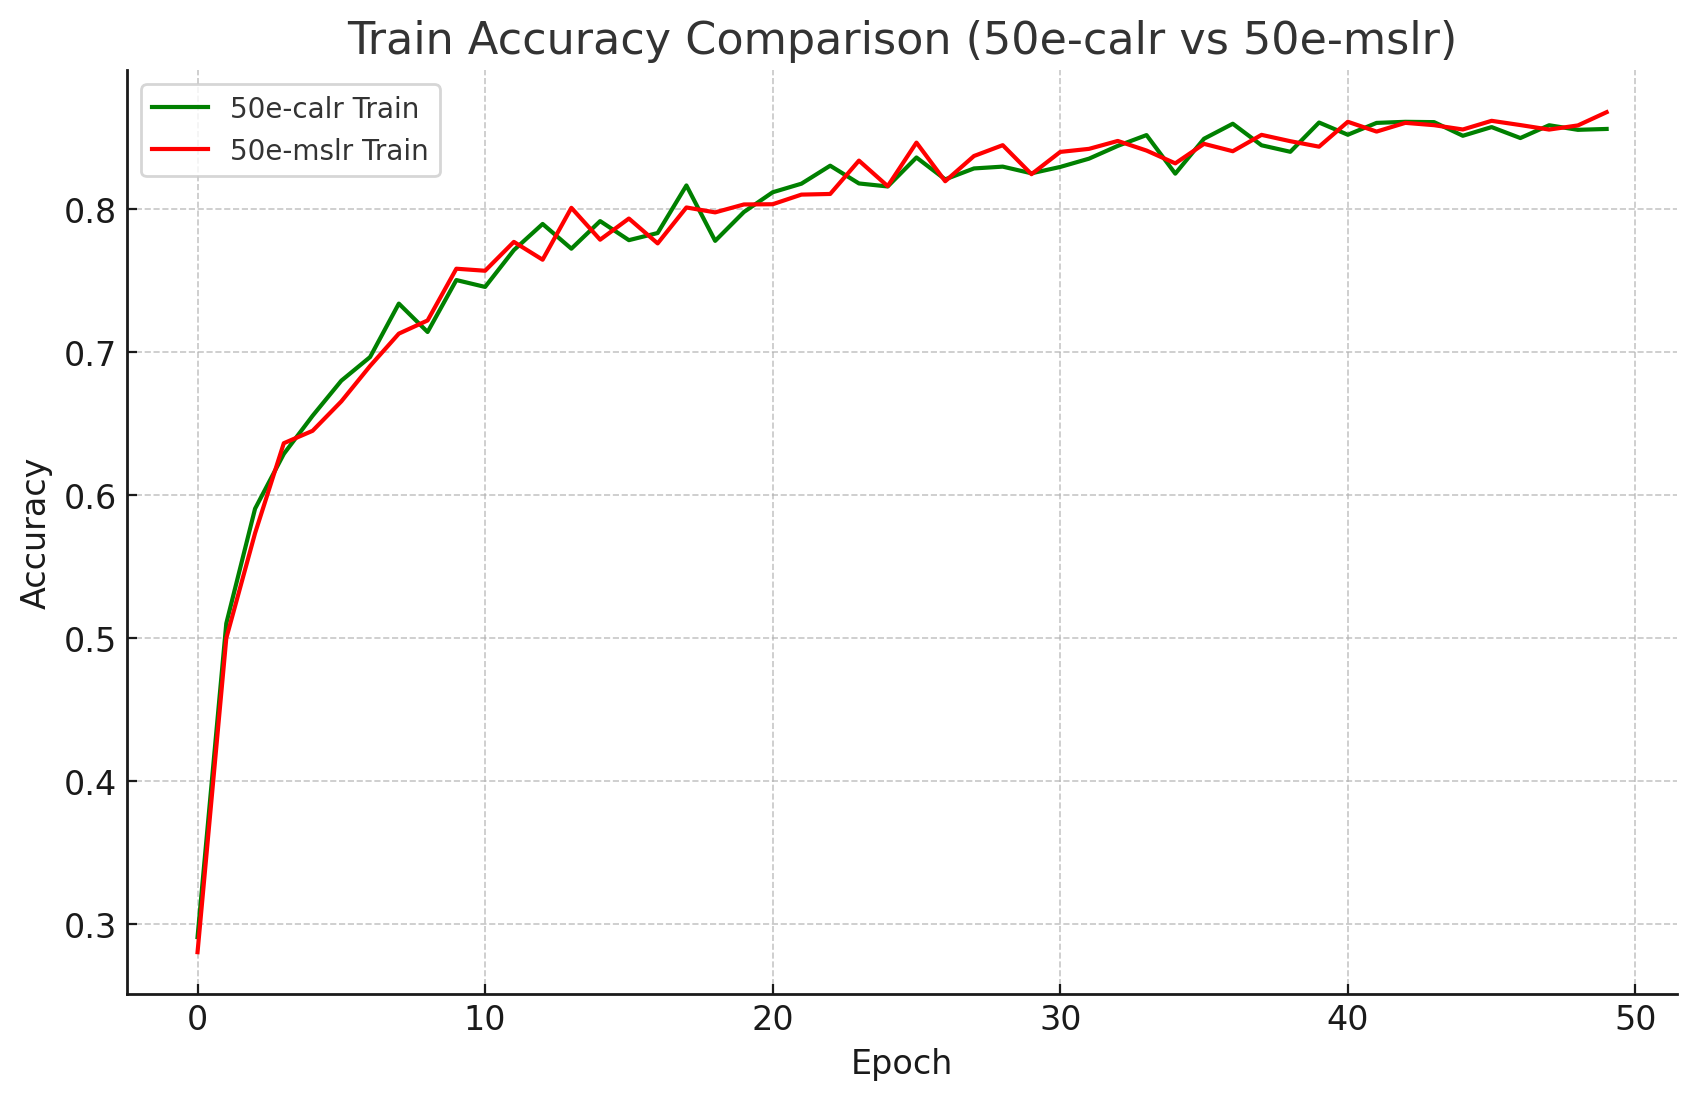
\includegraphics[width=\textwidth]{gambar/bab4-train-acc-50e.png}
    \caption{Accuracy (training) - 50 \emph{epoch}}
  \end{subfigure}
  \hfill
  \begin{subfigure}{0.45\textwidth}
    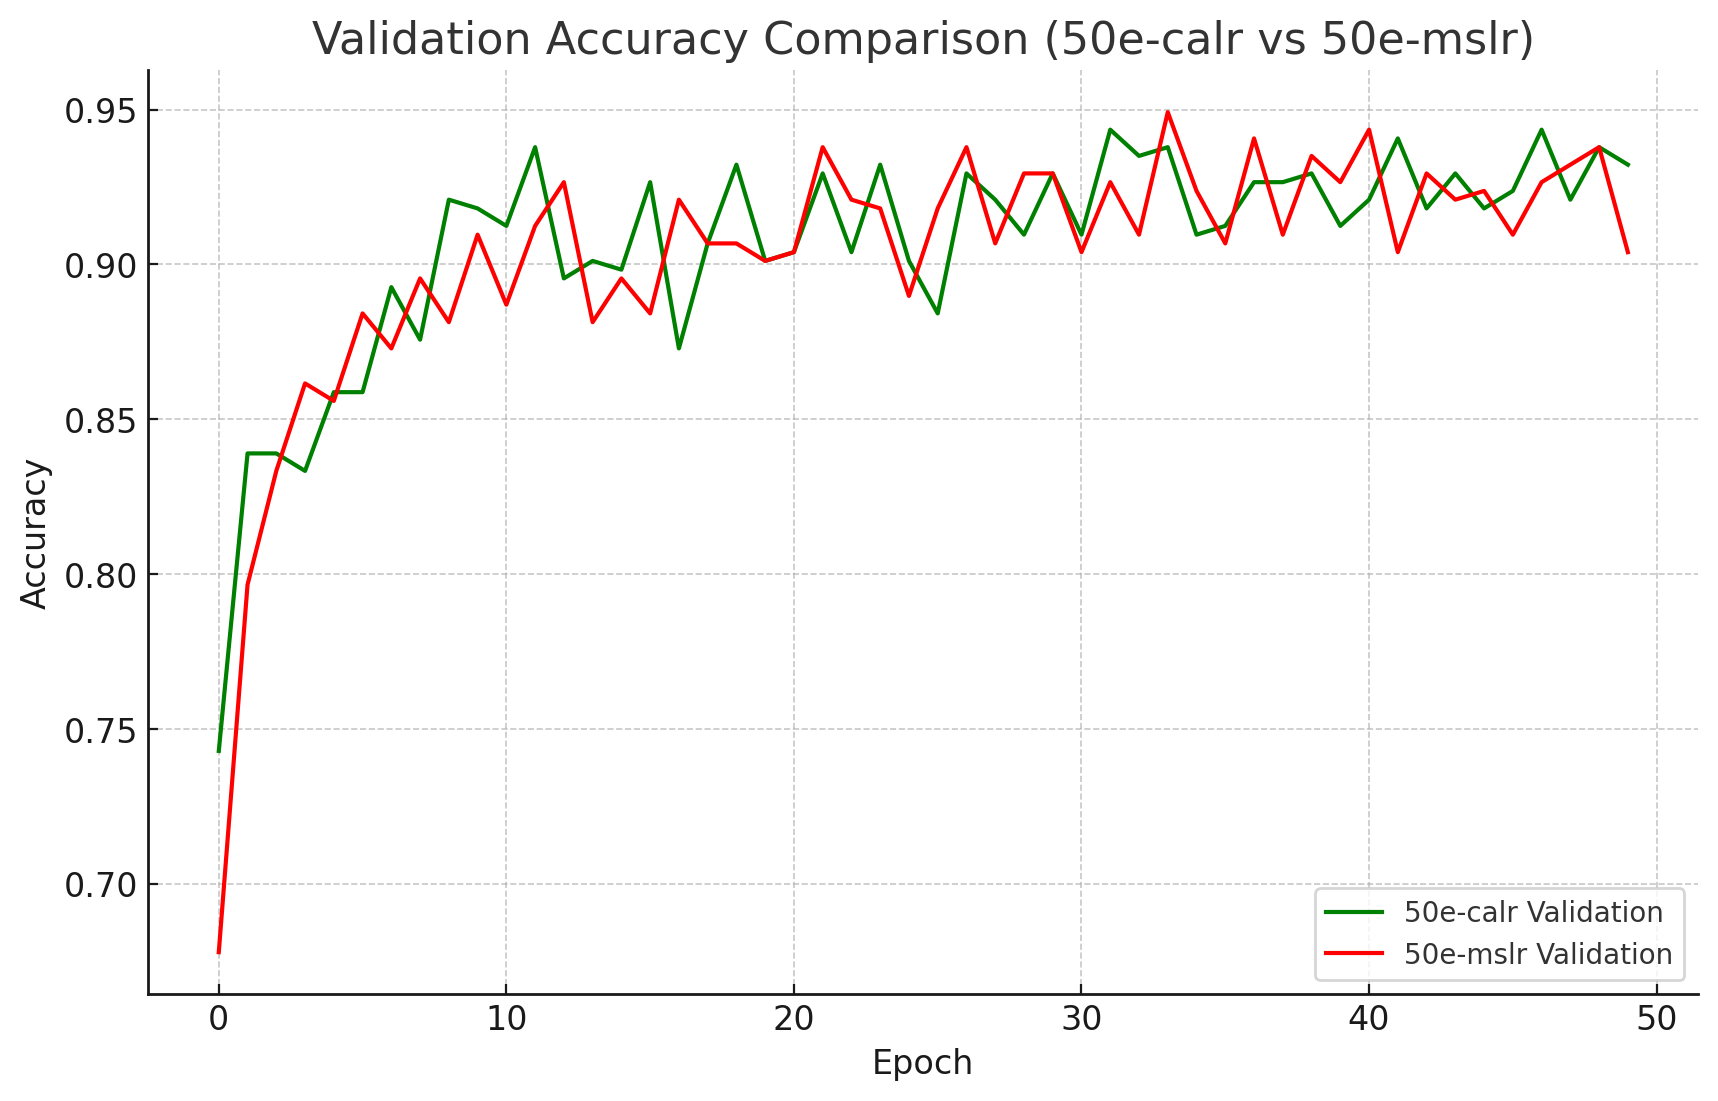
\includegraphics[width=\textwidth]{gambar/bab4-val-acc-50e.png}
    \caption{Accuracy (validation) - 50 \emph{epoch}}
  \end{subfigure}
  \caption{Kurva Accuracy selama proses pelatihan model SSD-MobileNetV2}
  \label{fig:accuracy_curves}
\end{figure}

\begin{figure}[htbp]
  \centering
  \begin{subfigure}{0.45\textwidth}
    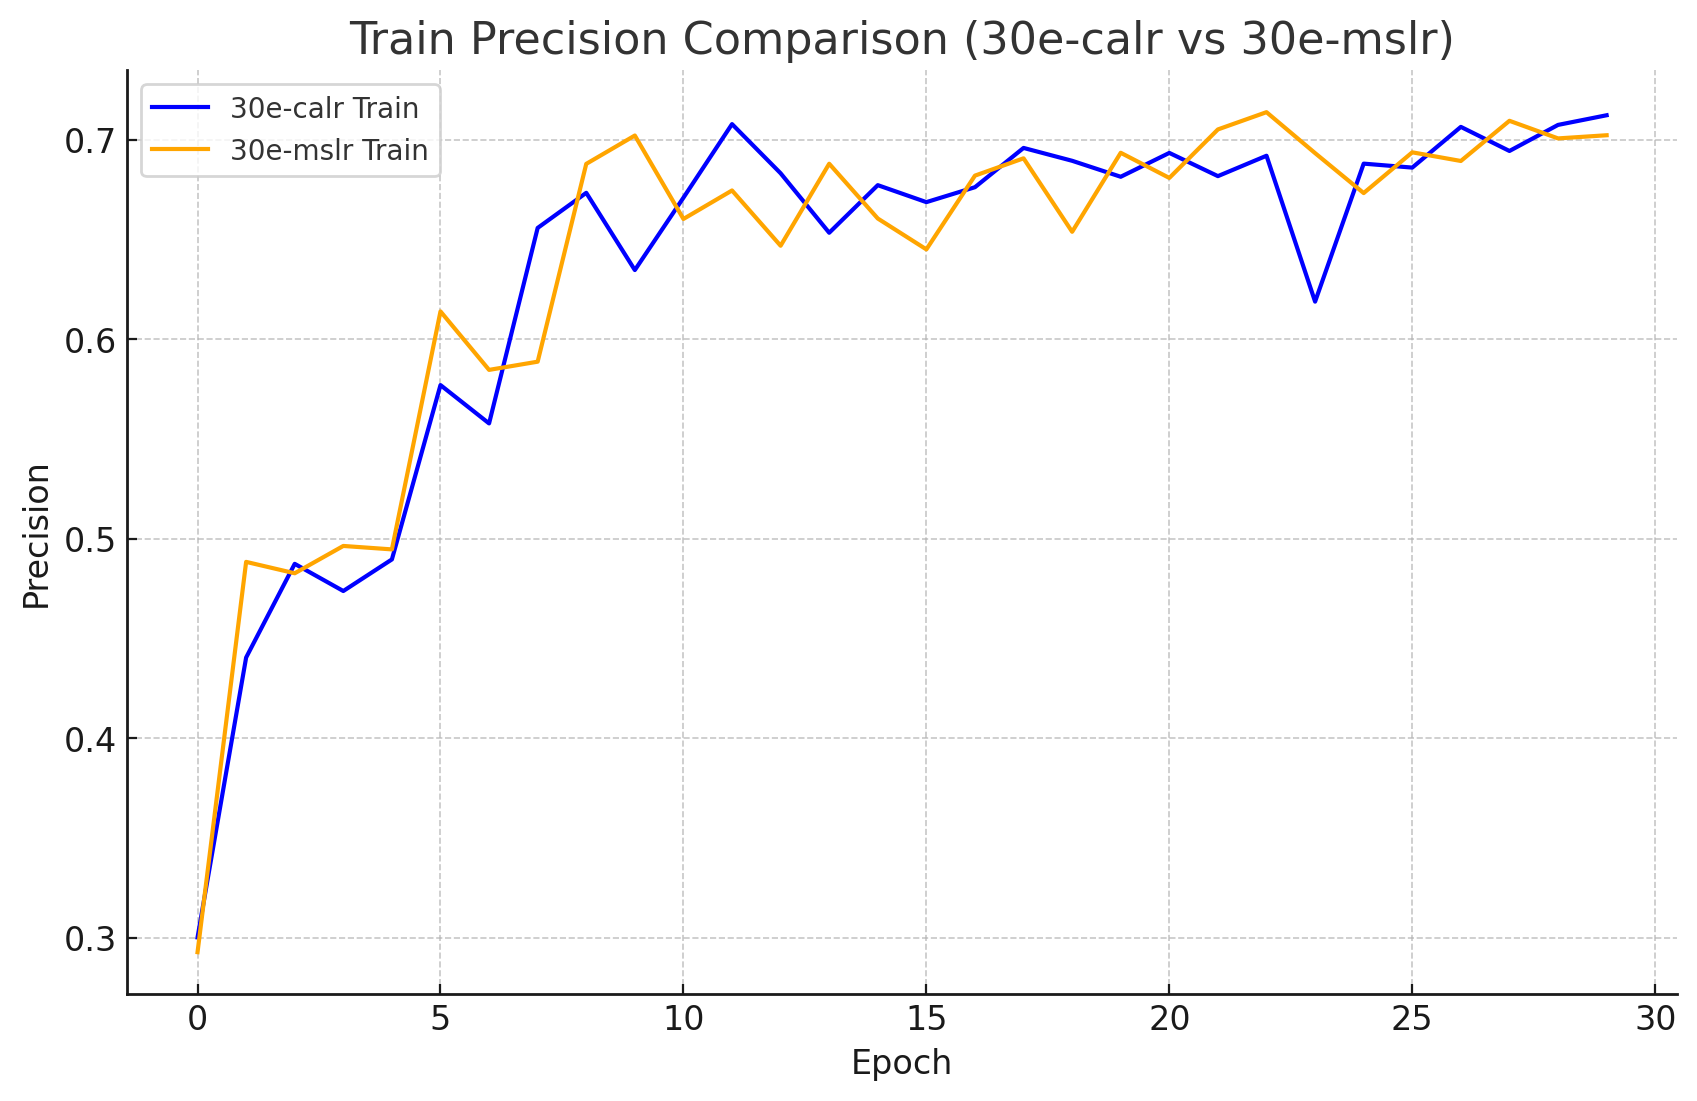
\includegraphics[width=\textwidth]{gambar/bab4-train-precision-30e.png}
    \caption{Precision (training) - 30 \emph{epoch}}
  \end{subfigure}
  \hfill
  \begin{subfigure}{0.45\textwidth}
    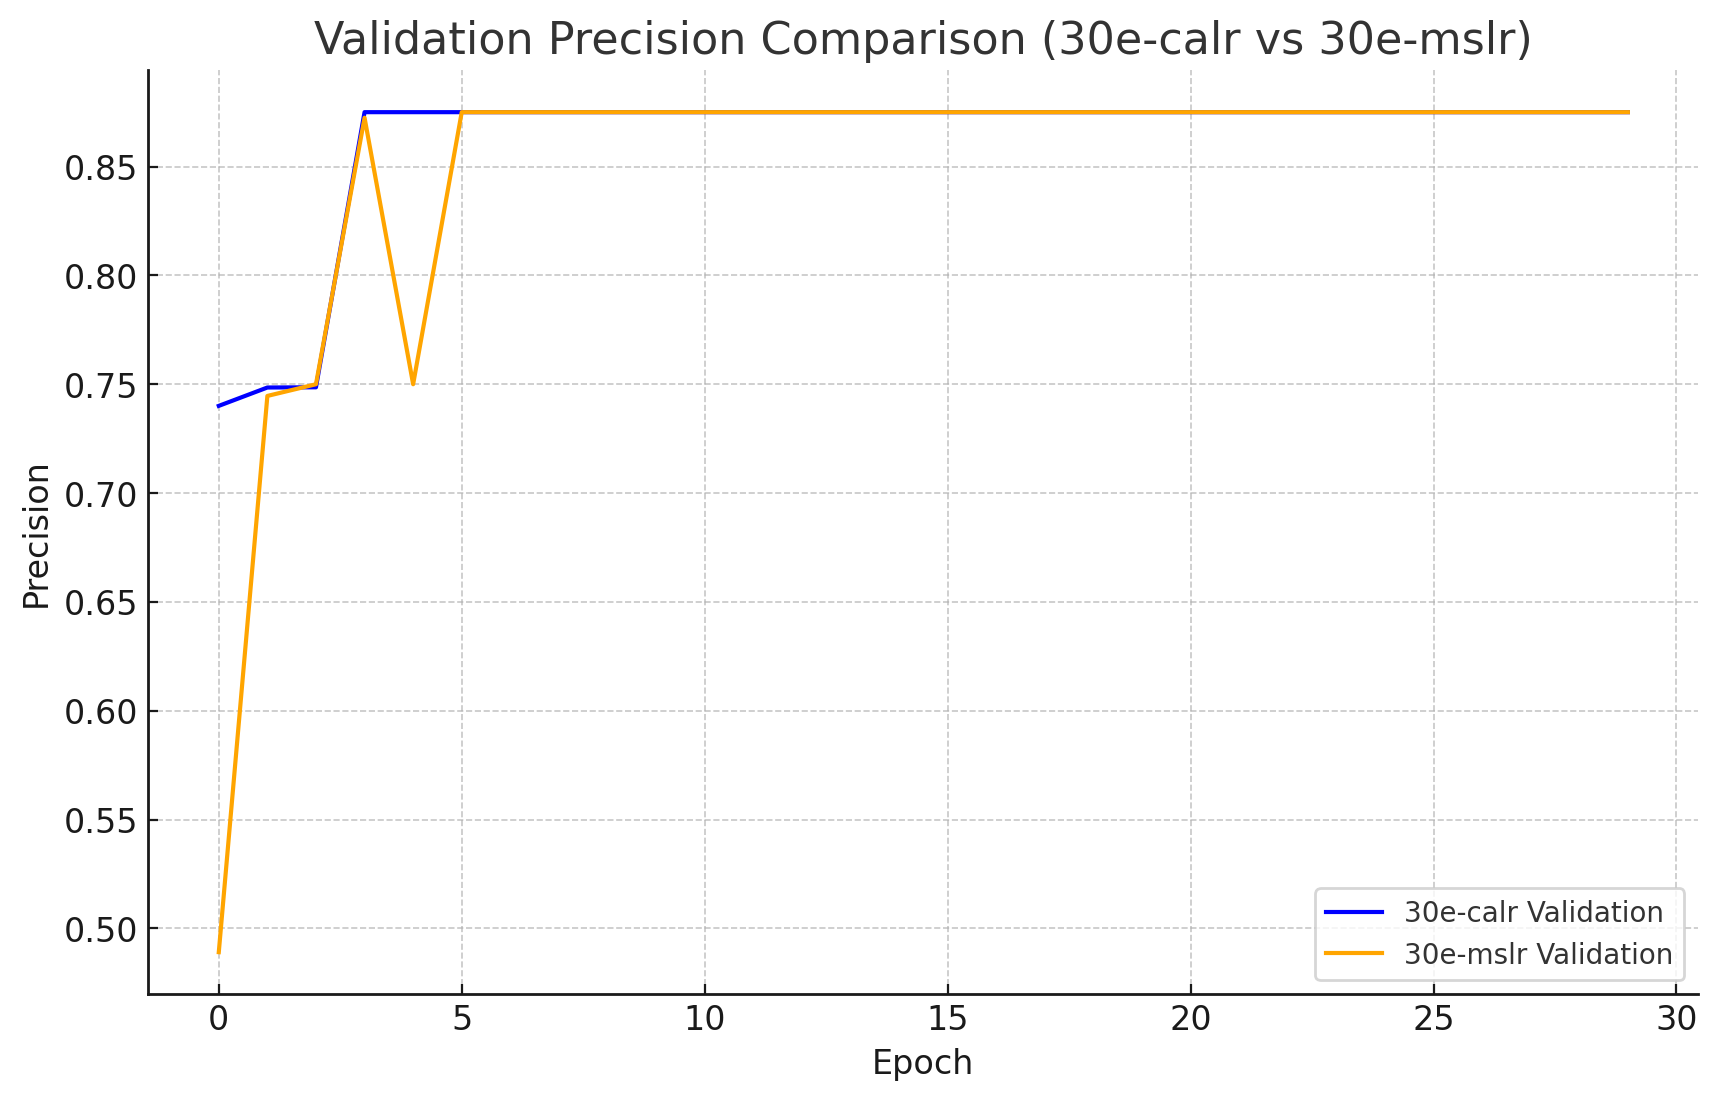
\includegraphics[width=\textwidth]{gambar/bab4-val-precision-30e.png}
    \caption{Precision (validation) - 30 \emph{epoch}}
  \end{subfigure}
  \hfill
  \begin{subfigure}{0.45\textwidth}
    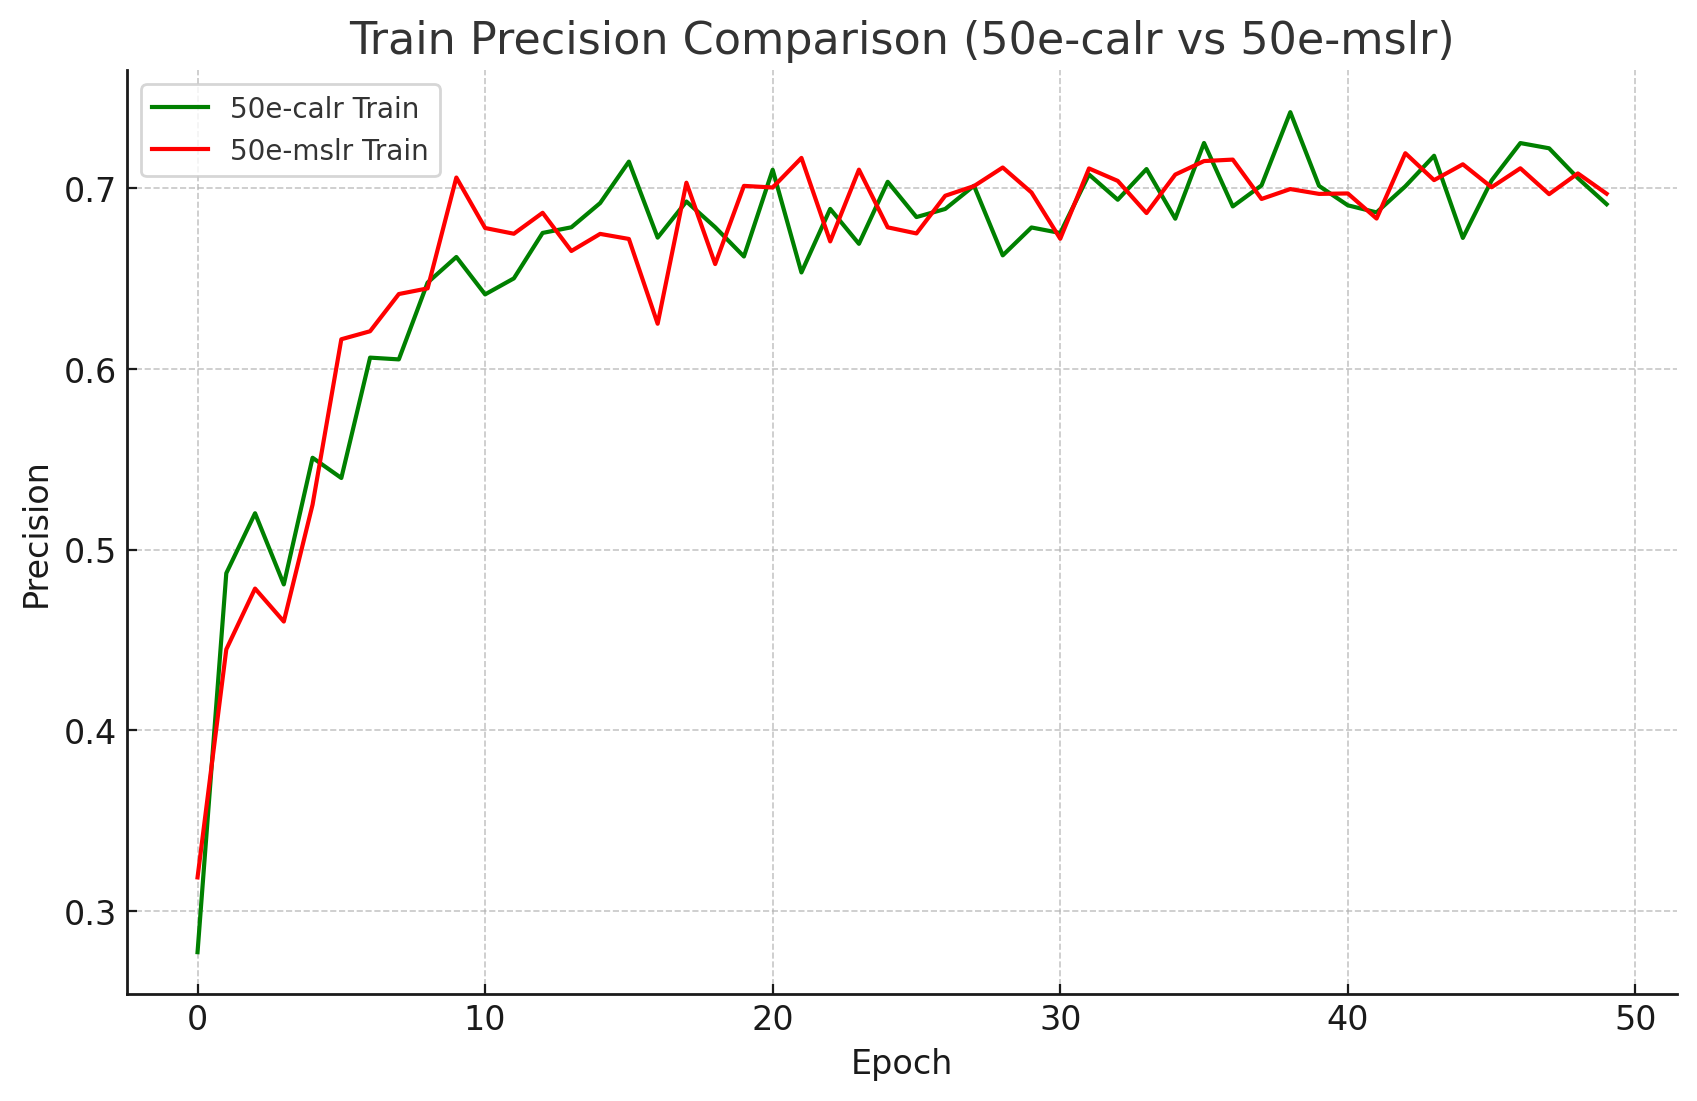
\includegraphics[width=\textwidth]{gambar/bab4-train-precision-50e.png}
    \caption{Precision (training) - 50 \emph{epoch}}
  \end{subfigure}
  \hfill
  \begin{subfigure}{0.45\textwidth}
    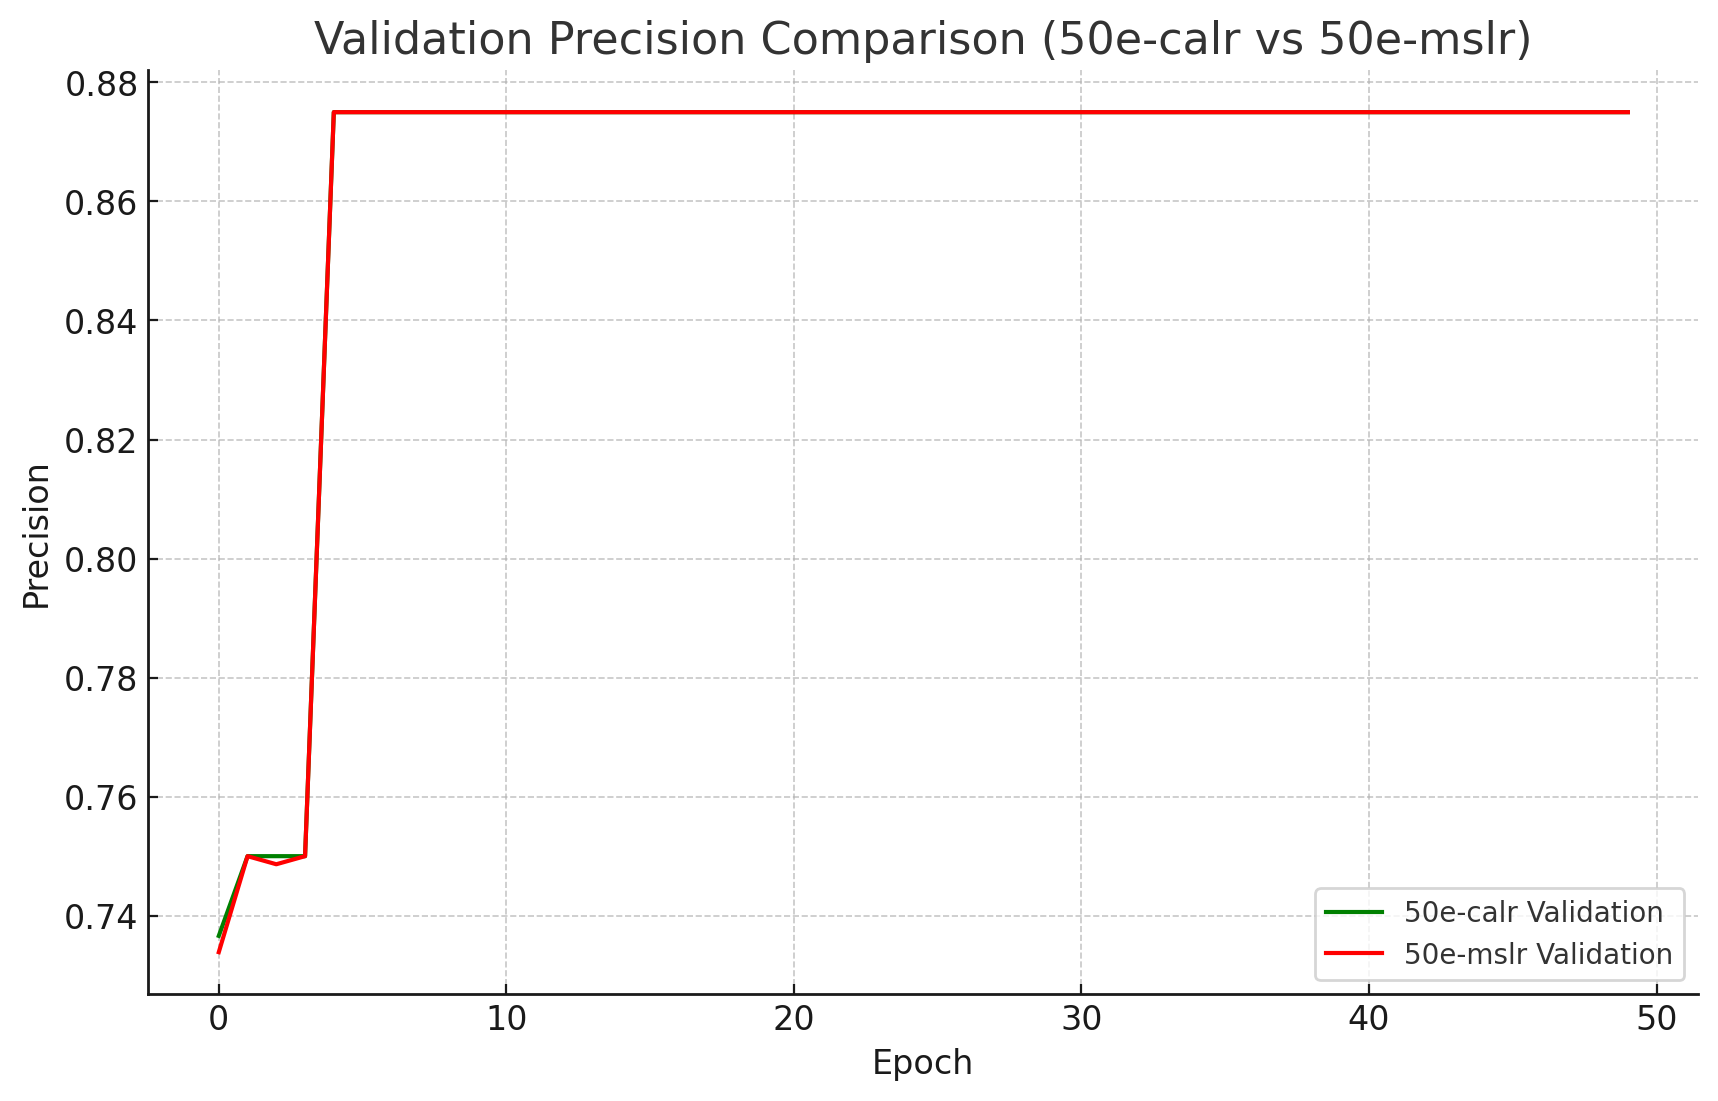
\includegraphics[width=\textwidth]{gambar/bab4-val-precision-50e.png}
    \caption{Precision (validation) - 50 \emph{epoch}}
  \end{subfigure}
  \caption{Kurva Precision selama proses pelatihan model SSD-MobileNetV2}
  \label{fig:precision_curves}
\end{figure}

\begin{figure}[htbp]
  \centering
  \begin{subfigure}{0.45\textwidth}
    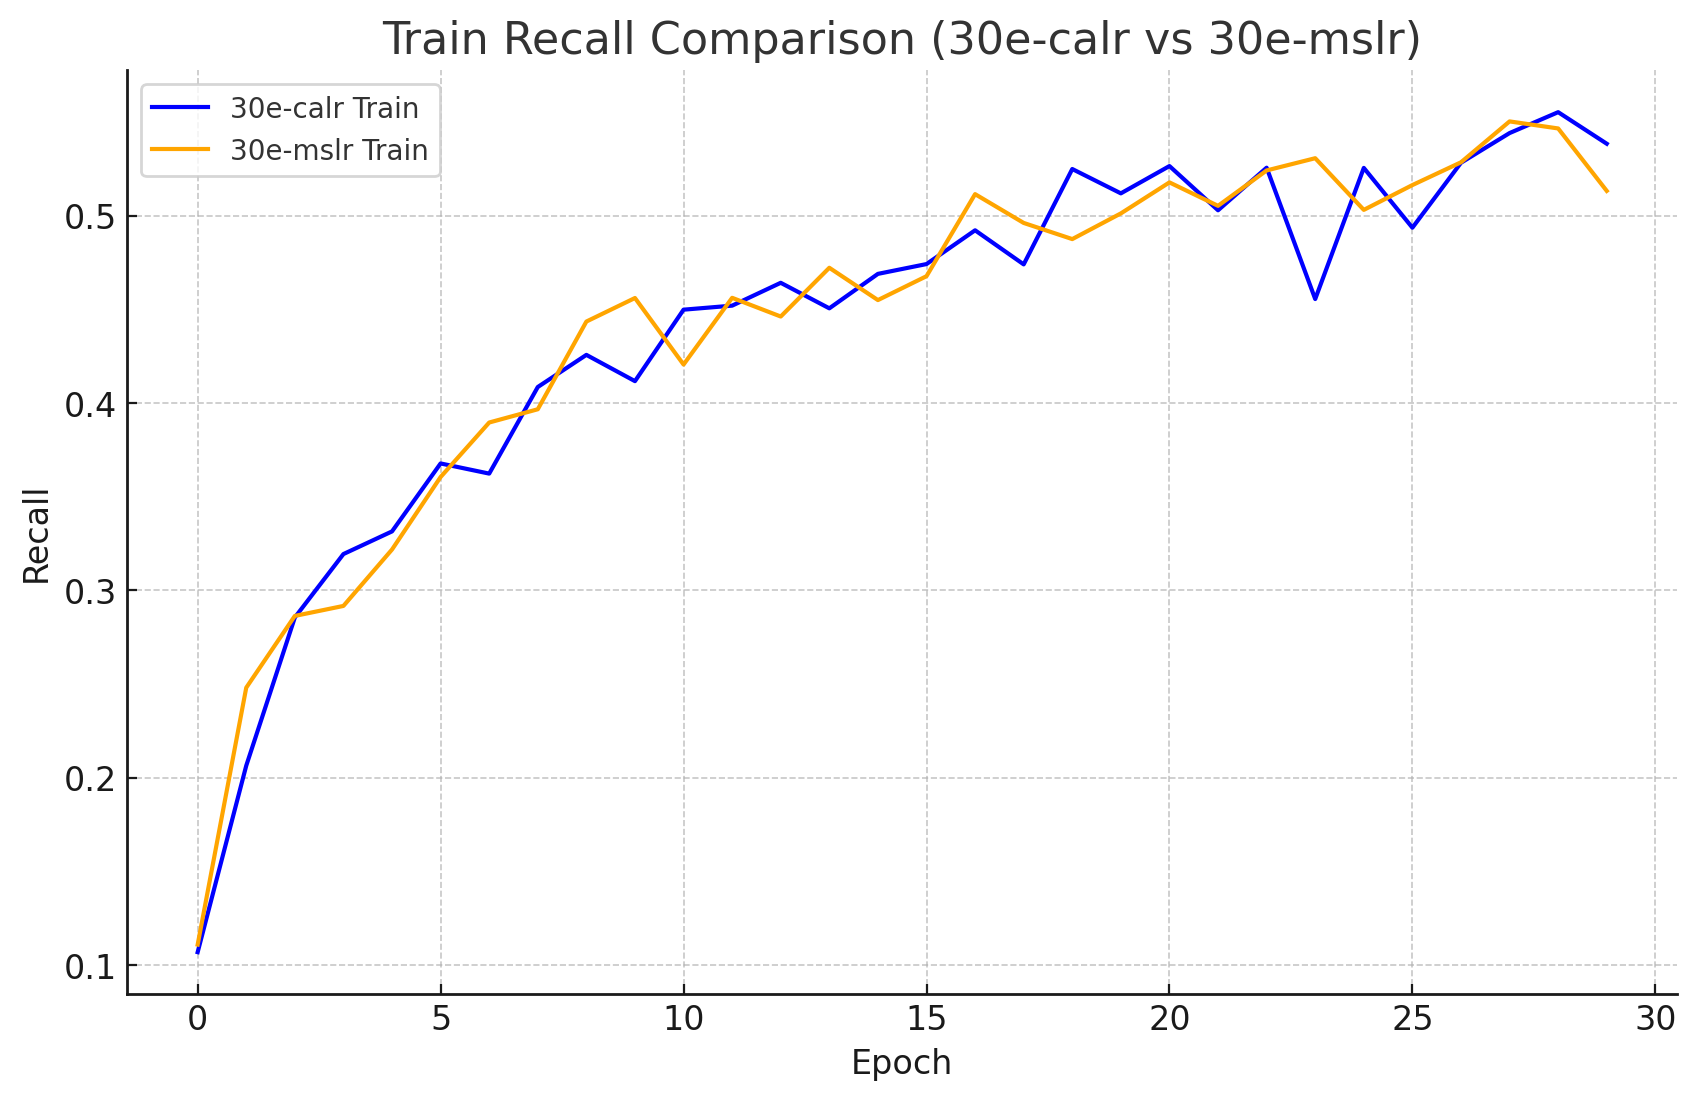
\includegraphics[width=\textwidth]{gambar/bab4-train-recall-30e.png}
    \caption{Recall (training) - 30 \emph{epoch}}
  \end{subfigure}
  \hfill
  \begin{subfigure}{0.45\textwidth}
    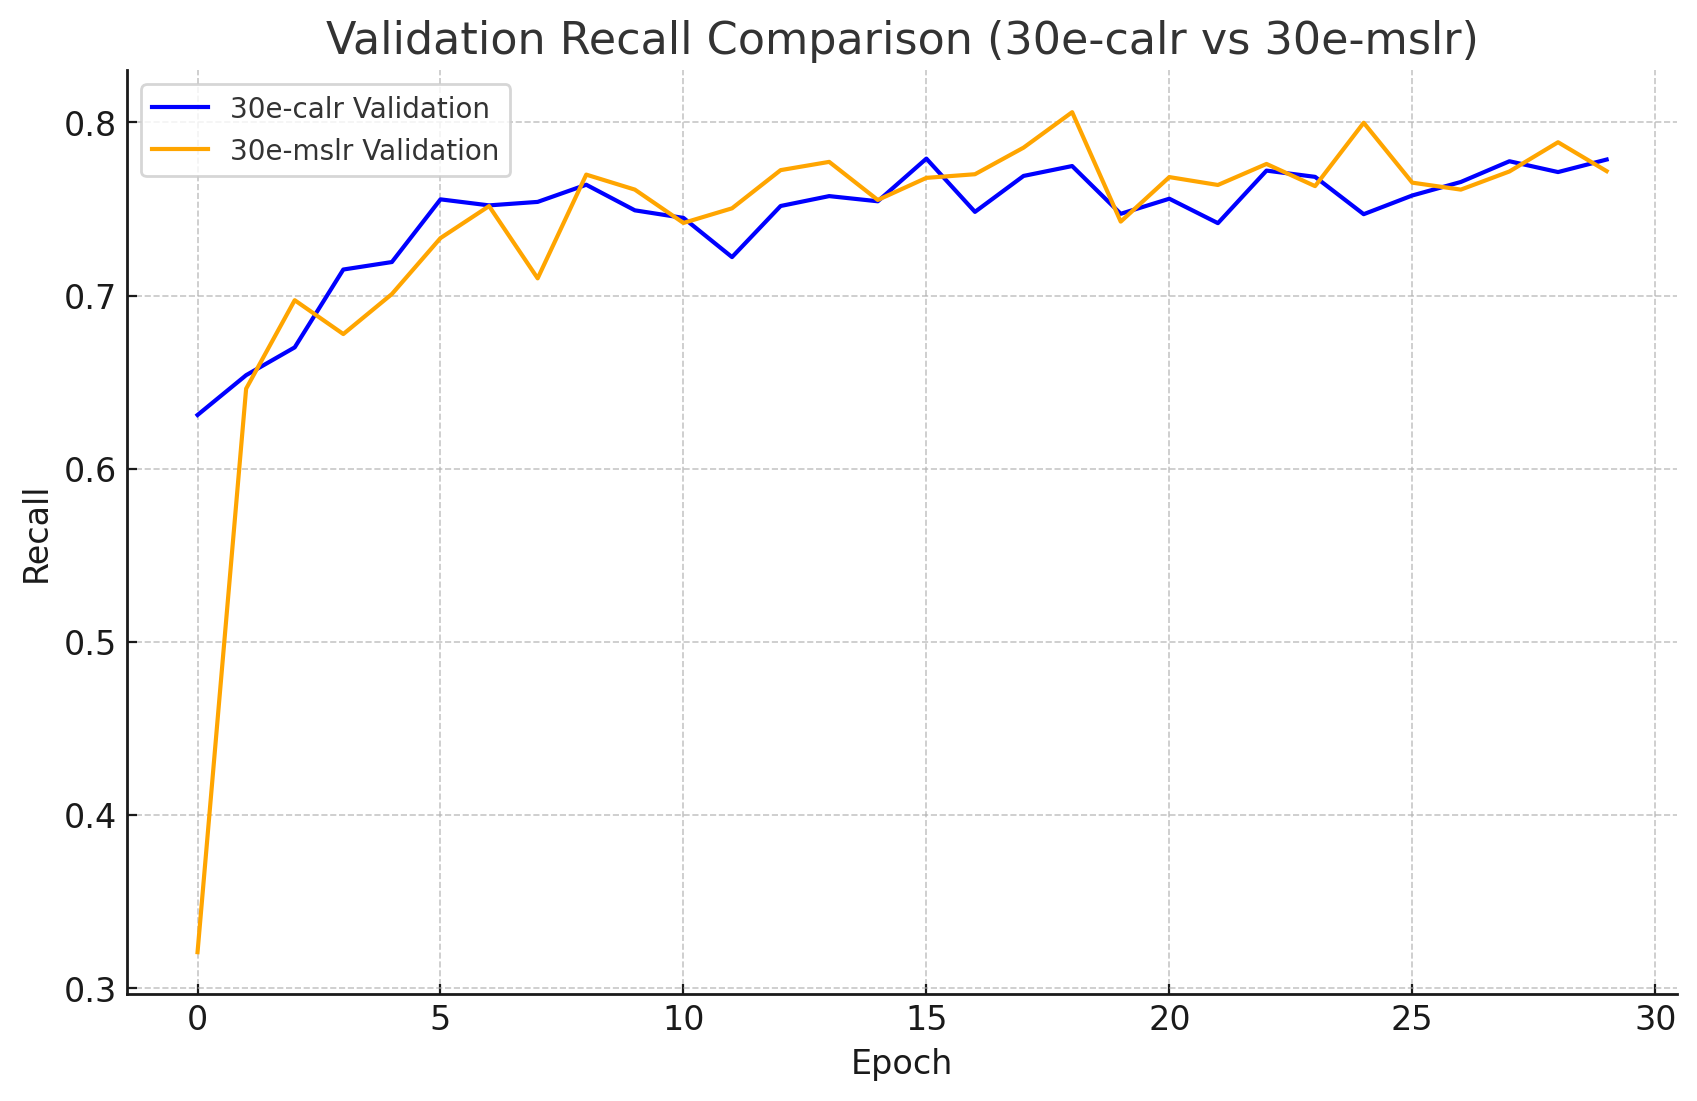
\includegraphics[width=\textwidth]{gambar/bab4-val-recall-30e.png}
    \caption{Recall (validation) - 30 \emph{epoch}}
  \end{subfigure}
  \hfill
  \begin{subfigure}{0.45\textwidth}
    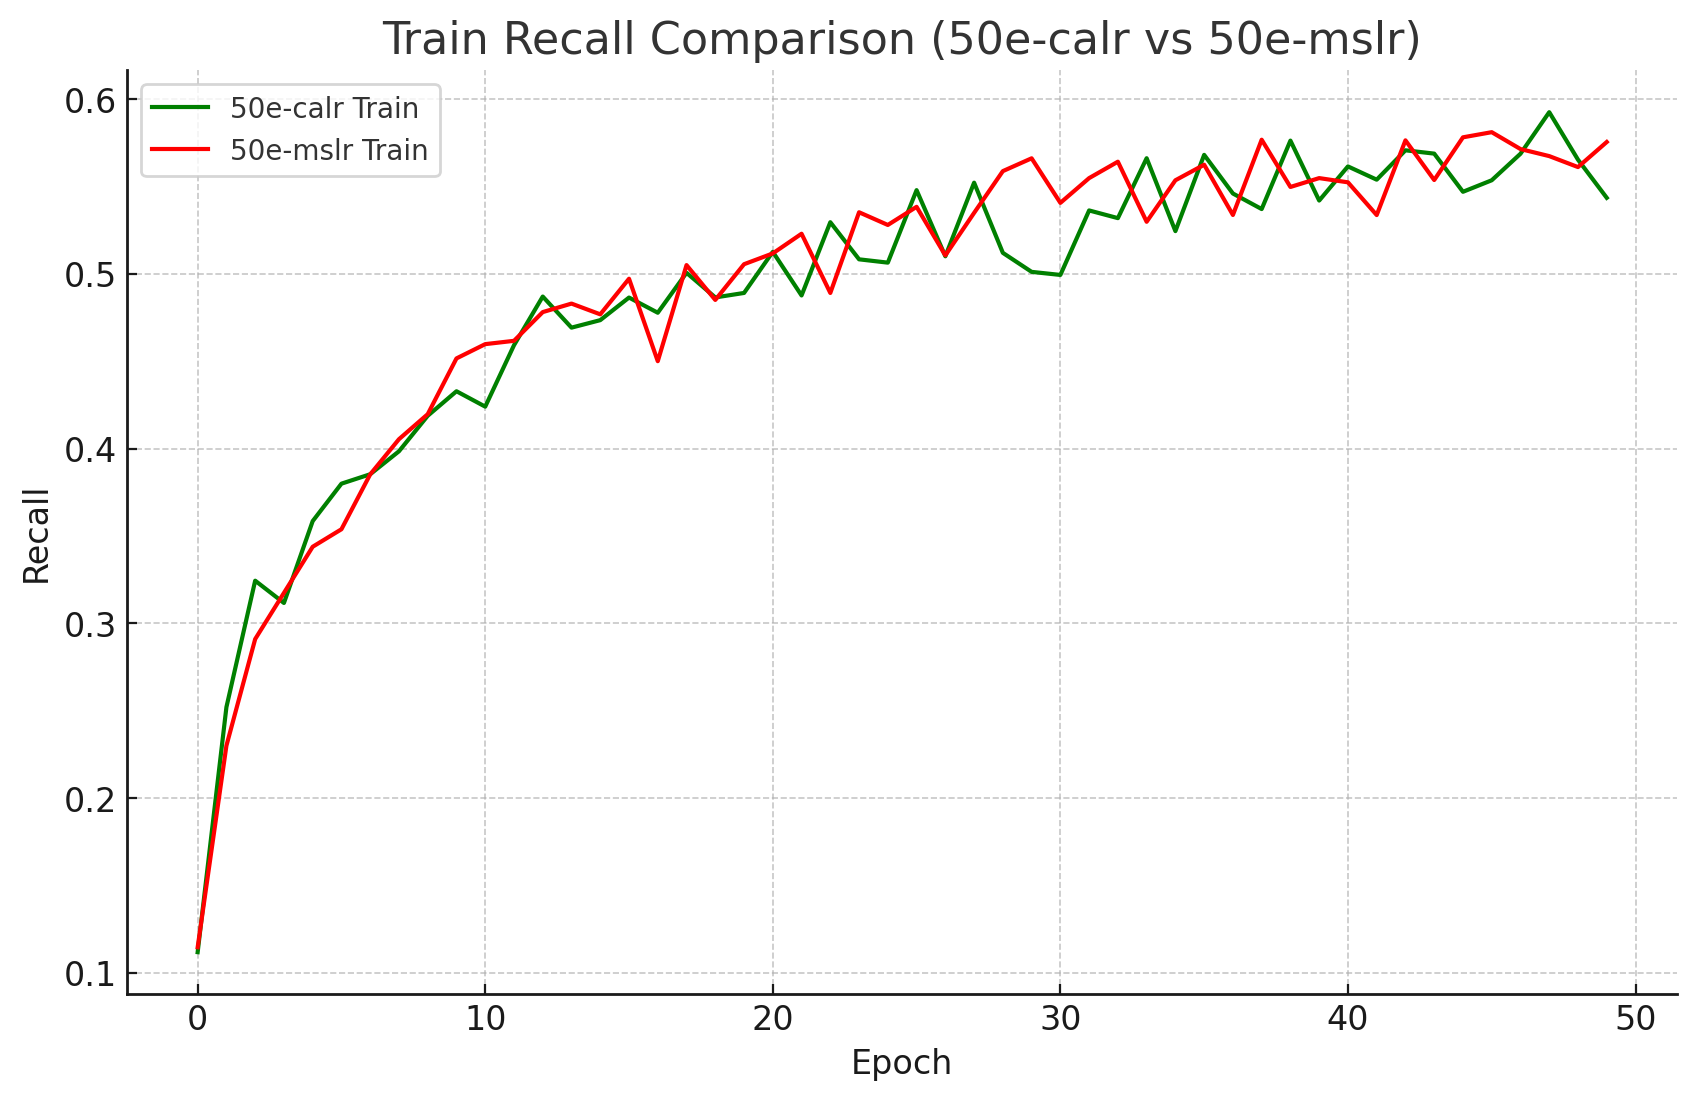
\includegraphics[width=\textwidth]{gambar/bab4-train-recall-50e.png}
    \caption{Recall (training) - 50 \emph{epoch}}
  \end{subfigure}
  \hfill
  \begin{subfigure}{0.45\textwidth}
    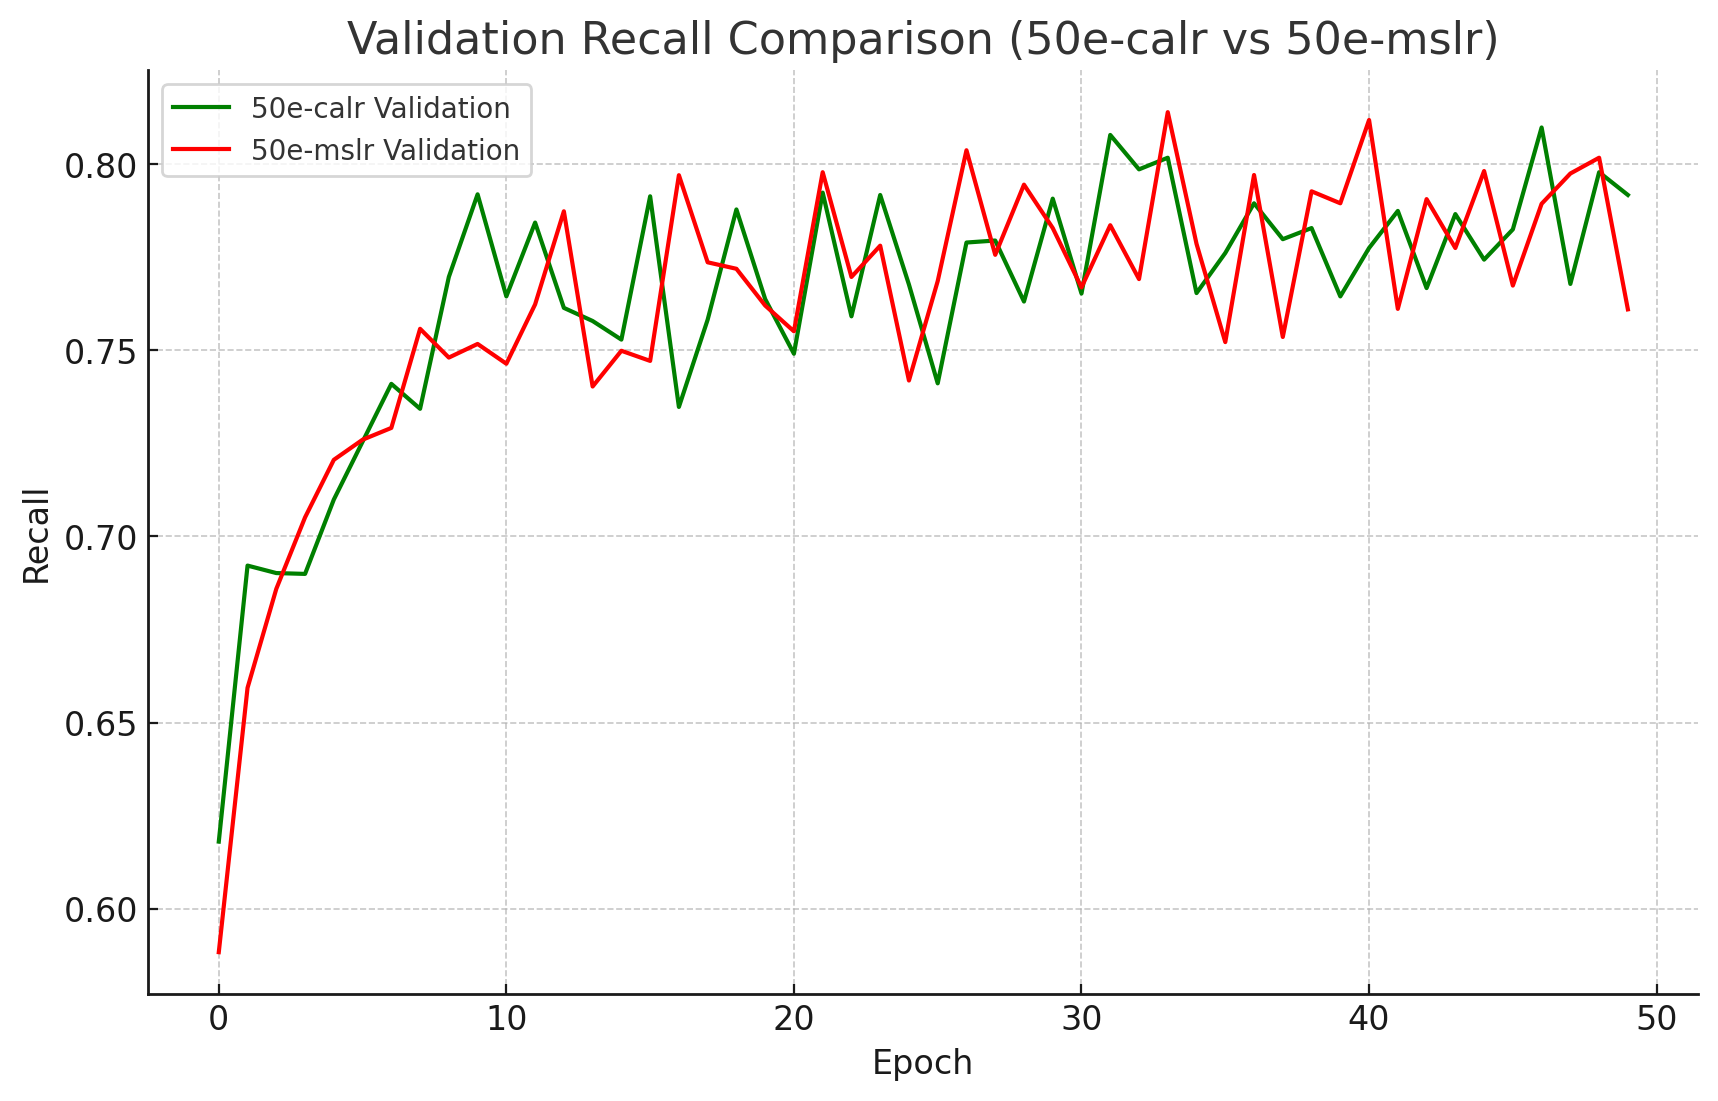
\includegraphics[width=\textwidth]{gambar/bab4-val-recall-50e.png}
    \caption{Recall (validation) - 50 \emph{epoch}}
  \end{subfigure}
  \caption{Kurva Recall selama proses pelatihan model SSD-MobileNetV2}
  \label{fig:recall_curves}
\end{figure}

\begin{figure}[htbp]
  \centering
  \begin{subfigure}{0.45\textwidth}
    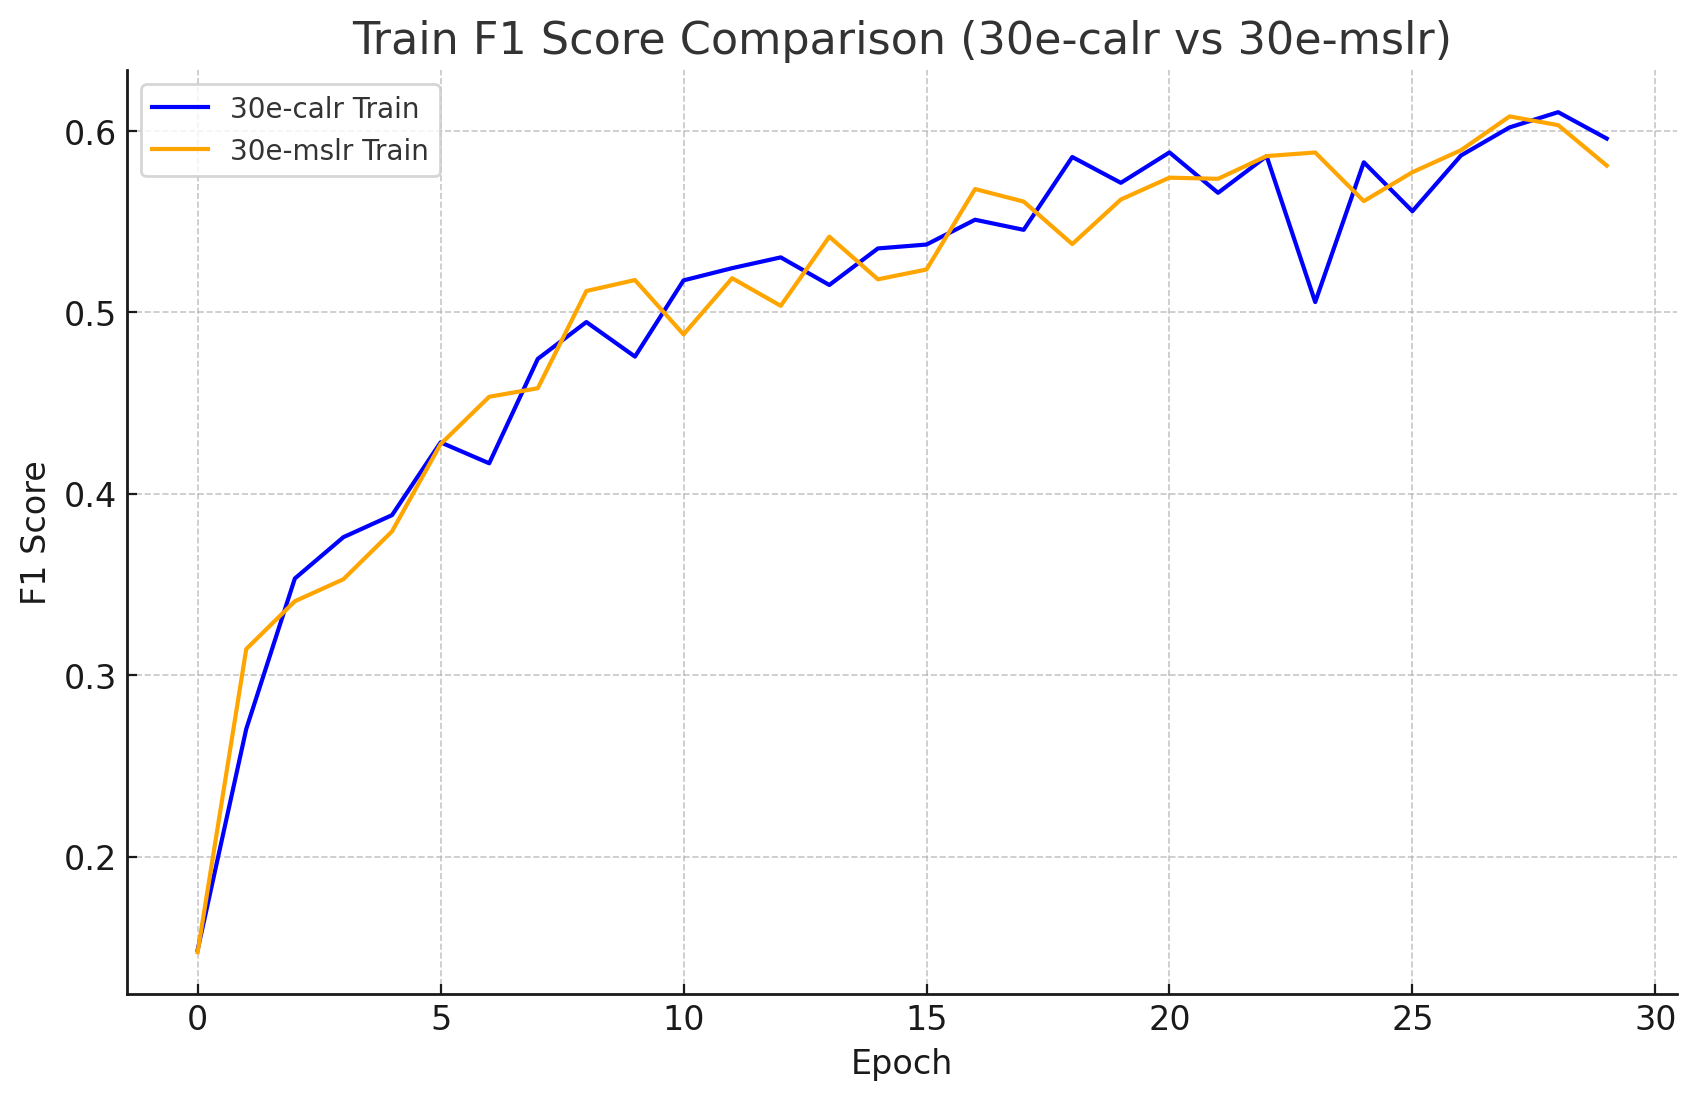
\includegraphics[width=\textwidth]{gambar/bab4-train-f1-score-30e.png}
    \caption{F1 Score (training) - 30 \emph{epoch}}
  \end{subfigure}
  \hfill
  \begin{subfigure}{0.45\textwidth}
    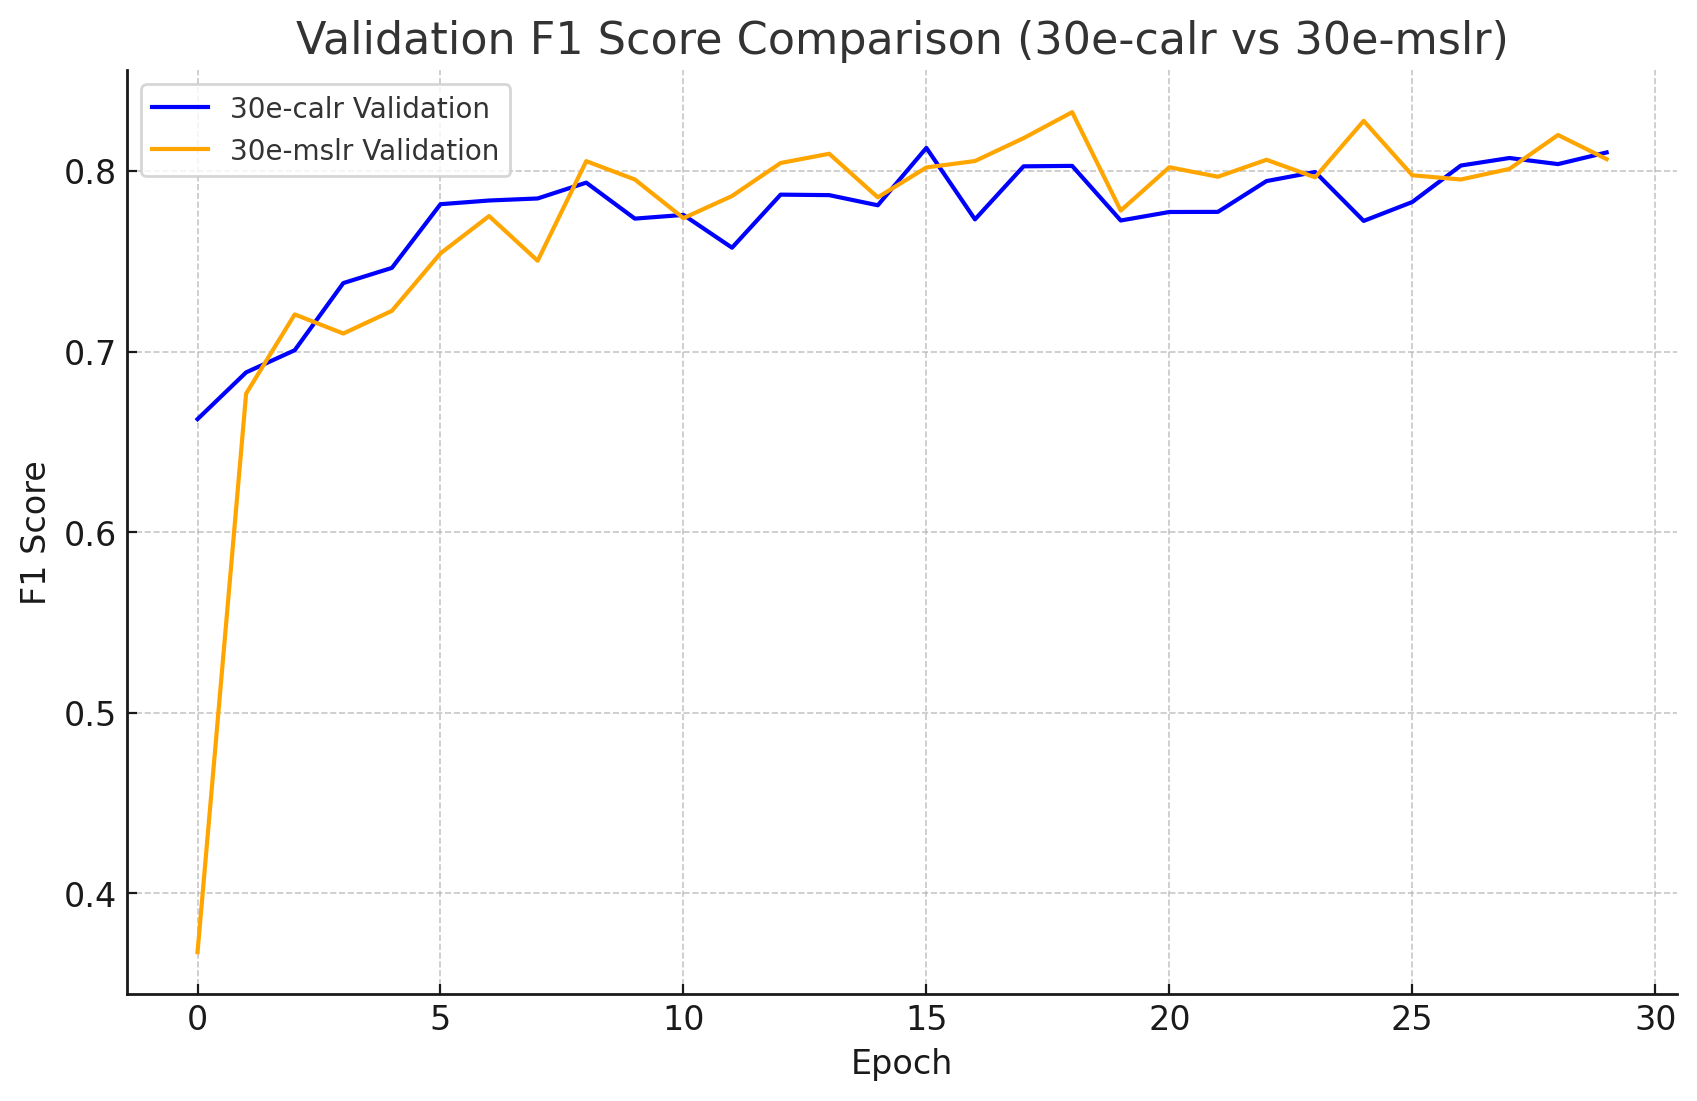
\includegraphics[width=\textwidth]{gambar/bab4-val-f1-score-30e.png}
    \caption{F1 Score (validation) - 30 \emph{epoch}}
  \end{subfigure}
  \hfill
  \begin{subfigure}{0.45\textwidth}
    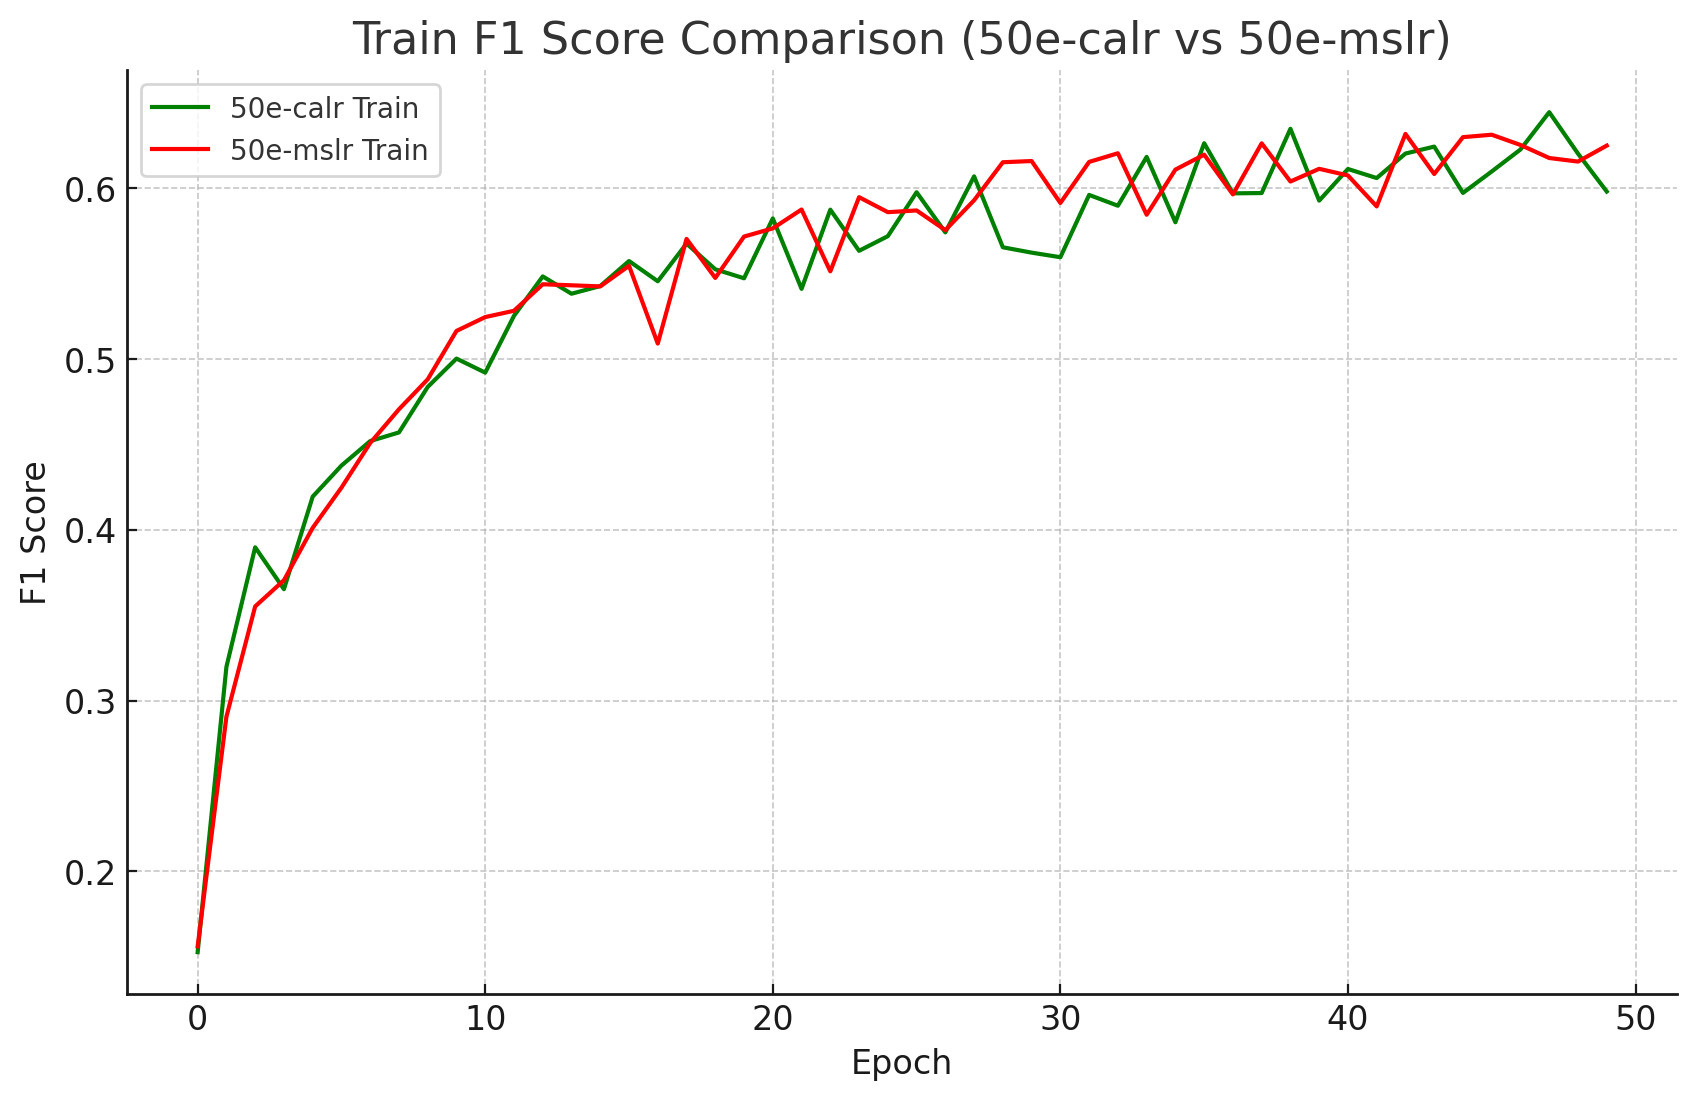
\includegraphics[width=\textwidth]{gambar/bab4-train-f1-score-50e.png}
    \caption{F1 Score (training) - 50 \emph{epoch}}
  \end{subfigure}
  \hfill
  \begin{subfigure}{0.45\textwidth}
    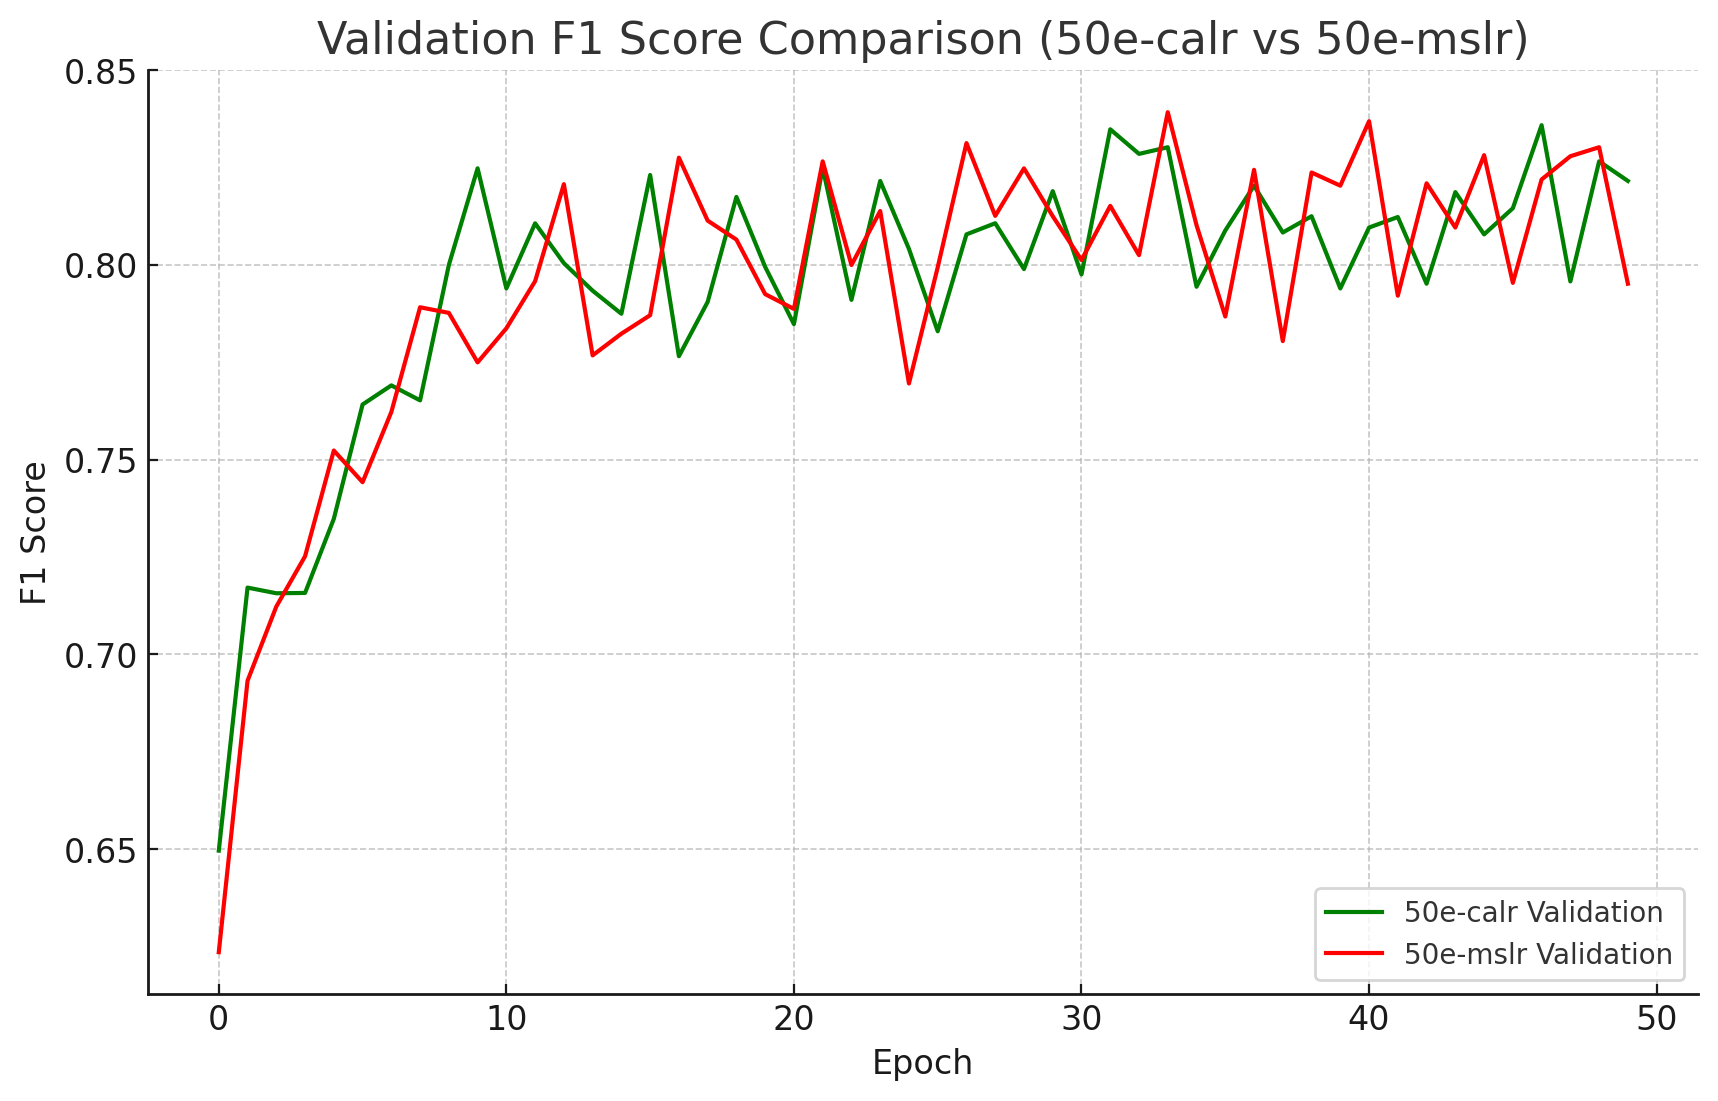
\includegraphics[width=\textwidth]{gambar/bab4-val-f1-score-50e.png}
    \caption{F1 Score (validation) - 50 \emph{epoch}}
  \end{subfigure}
  \caption{Kurva F1 Score selama proses pelatihan model SSD-MobileNetV2}
  \label{fig:f1_score_curves}
\end{figure}

\begin{figure}[htbp]
  \centering
  \begin{subfigure}{0.45\textwidth}
    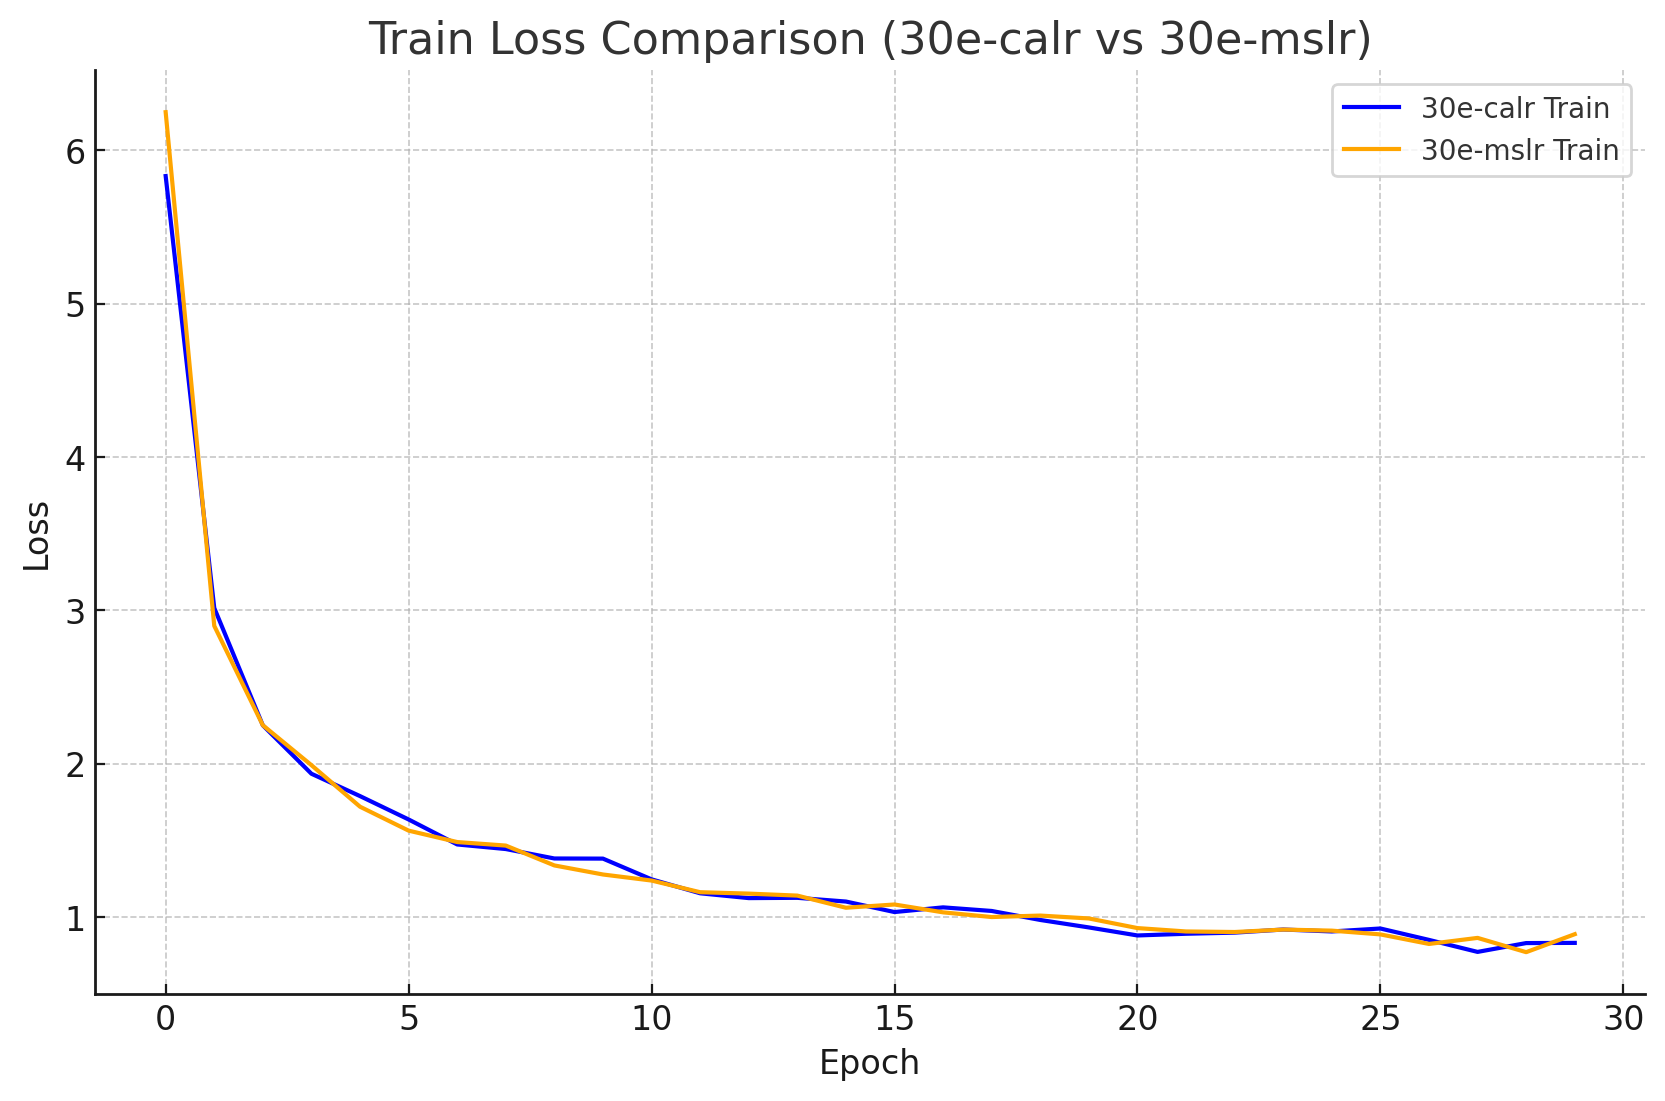
\includegraphics[width=\textwidth]{gambar/bab4-train-loss-30e.png}
    \caption{Loss (training) - 30 \emph{epoch}}
  \end{subfigure}
  \hfill
  \begin{subfigure}{0.45\textwidth}
    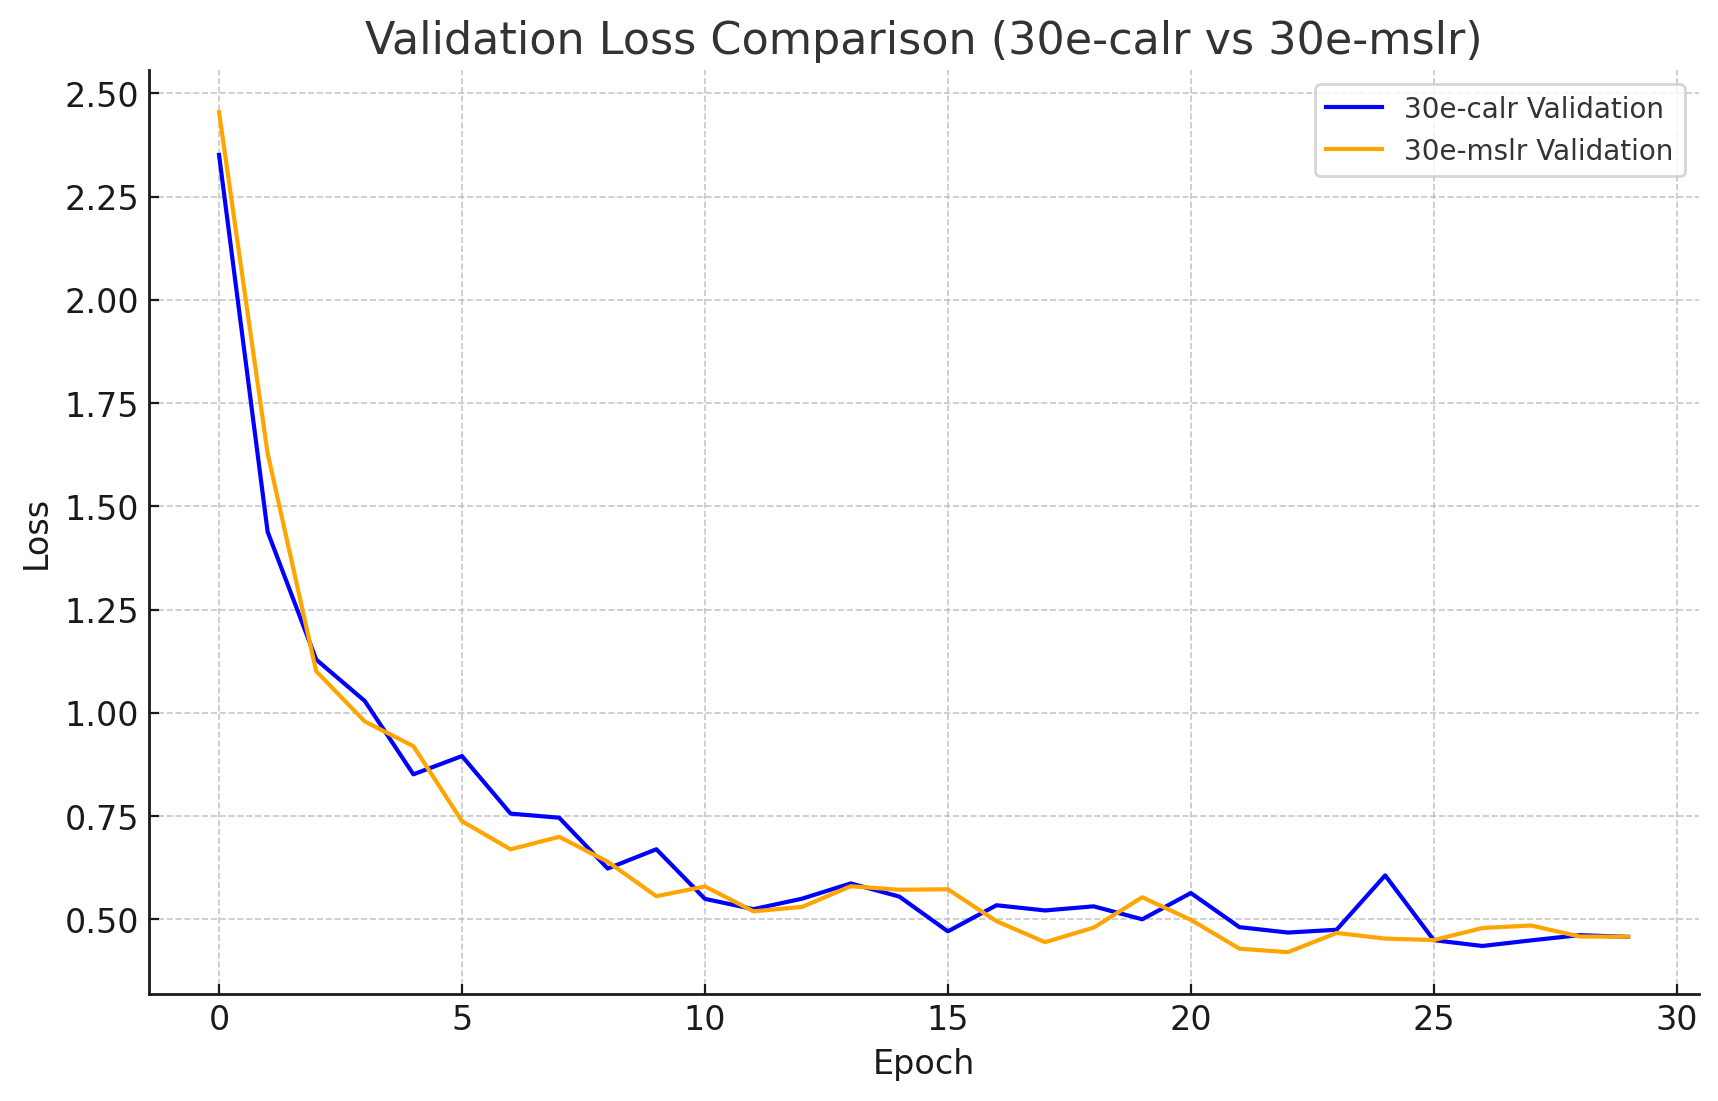
\includegraphics[width=\textwidth]{gambar/bab4-val-loss-30e.png}
    \caption{Loss (validation) - 30 \emph{epoch}}
  \end{subfigure}
  \hfill
  \begin{subfigure}{0.45\textwidth}
    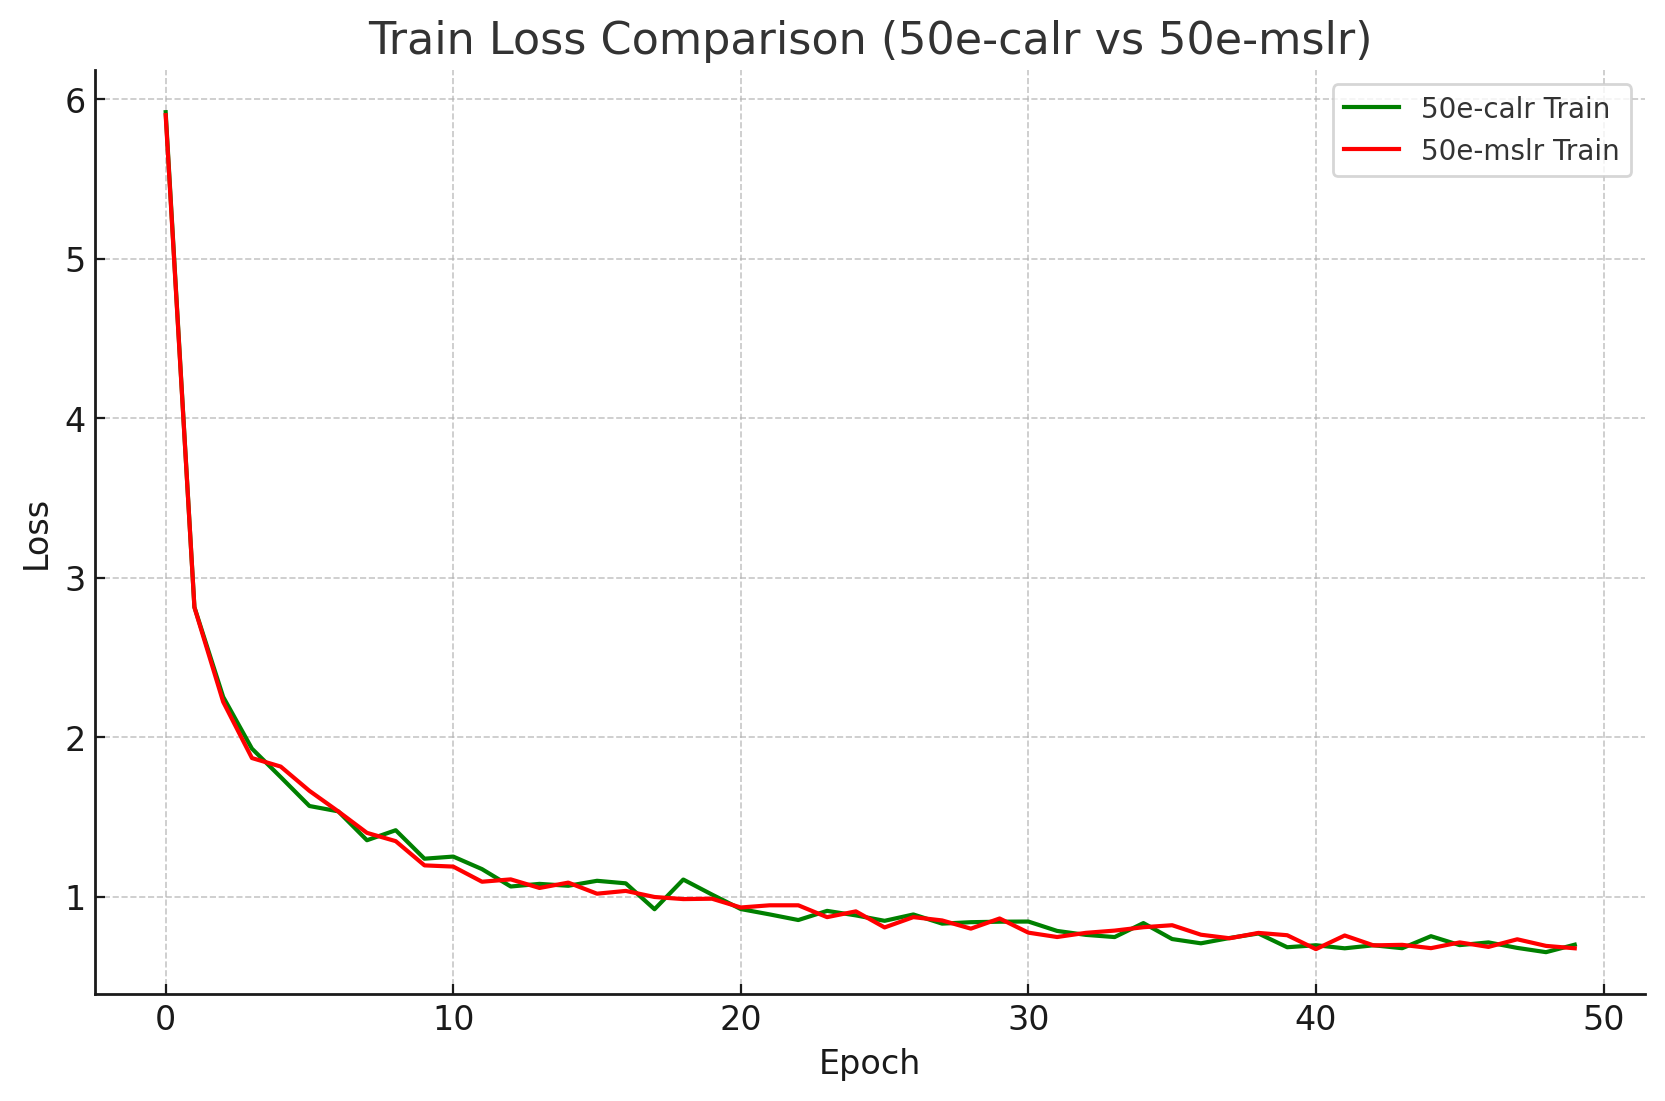
\includegraphics[width=\textwidth]{gambar/bab4-train-loss-50e.png}
    \caption{Loss (training) - 50 \emph{epoch}}
  \end{subfigure}
  \hfill
  \begin{subfigure}{0.45\textwidth}
    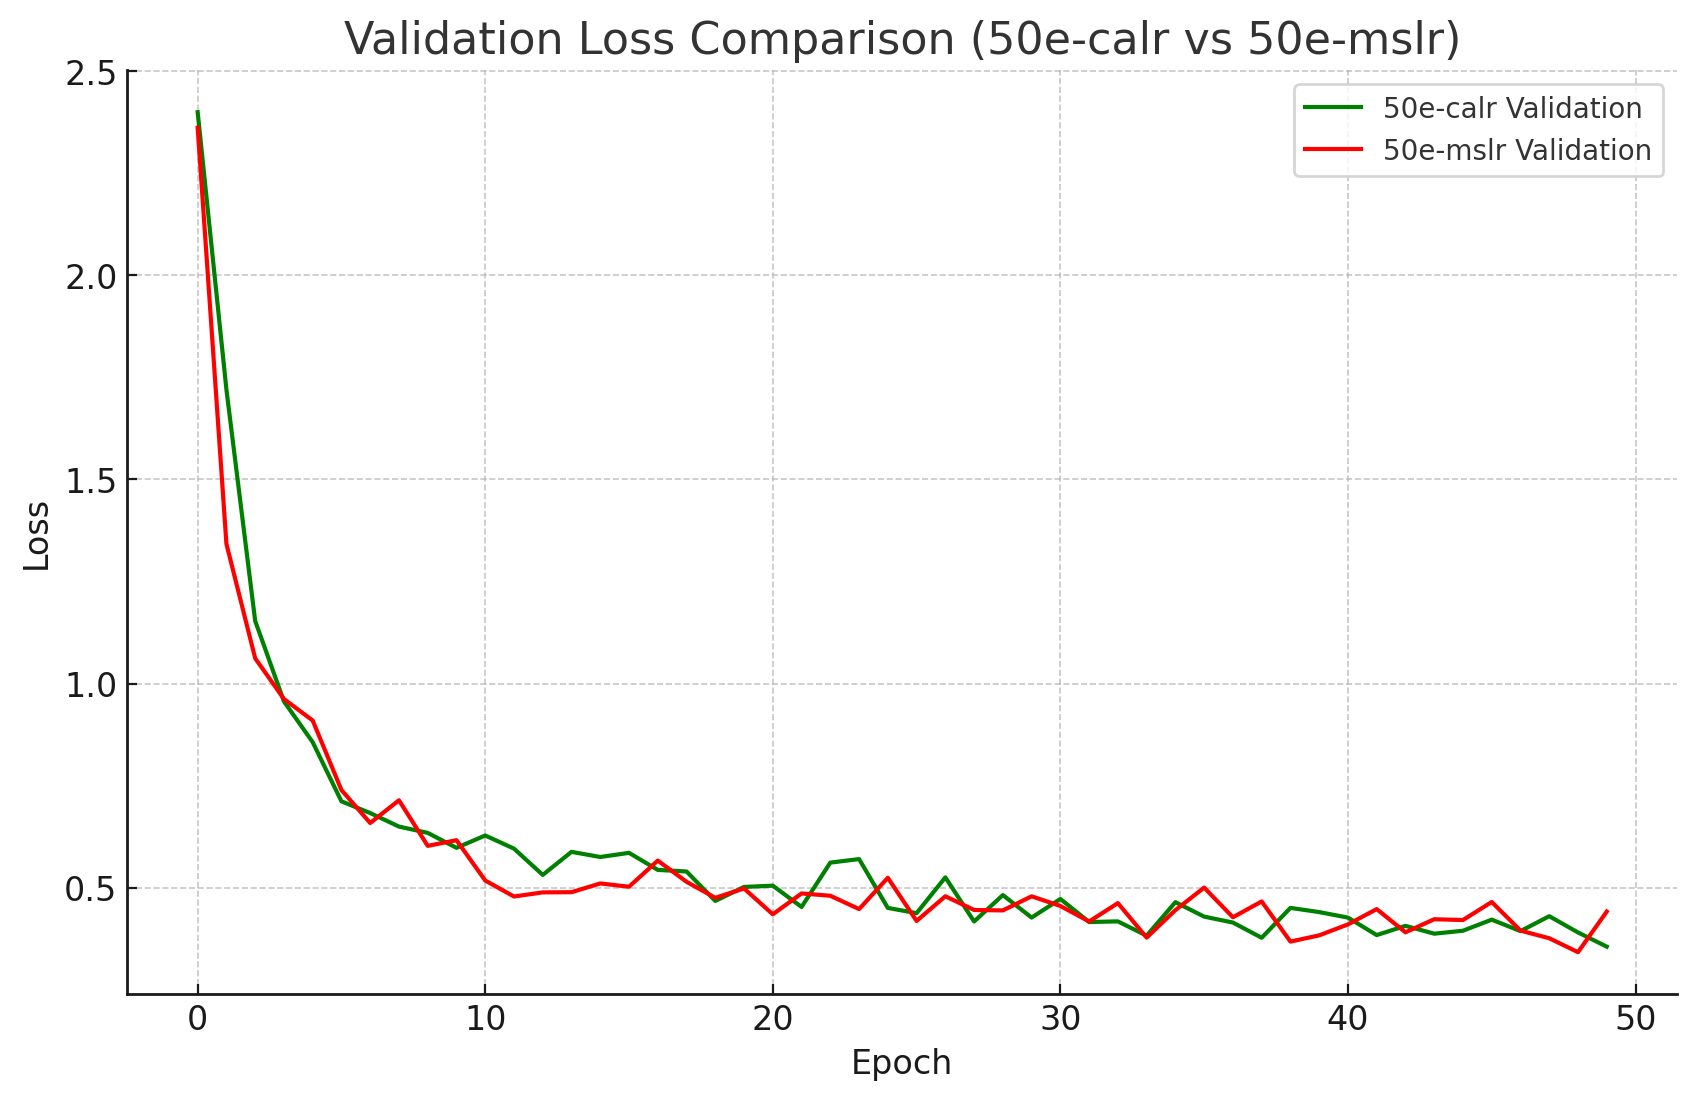
\includegraphics[width=\textwidth]{gambar/bab4-val-loss-50e.png}
    \caption{Loss (validation) - 50 \emph{epoch}}
  \end{subfigure}
  \caption{Kurva Loss selama proses pelatihan model SSD-MobileNetV2}
  \label{fig:loss_curves}
\end{figure}

\begin{figure}[htbp]
  \centering
  \begin{subfigure}{0.45\textwidth}
    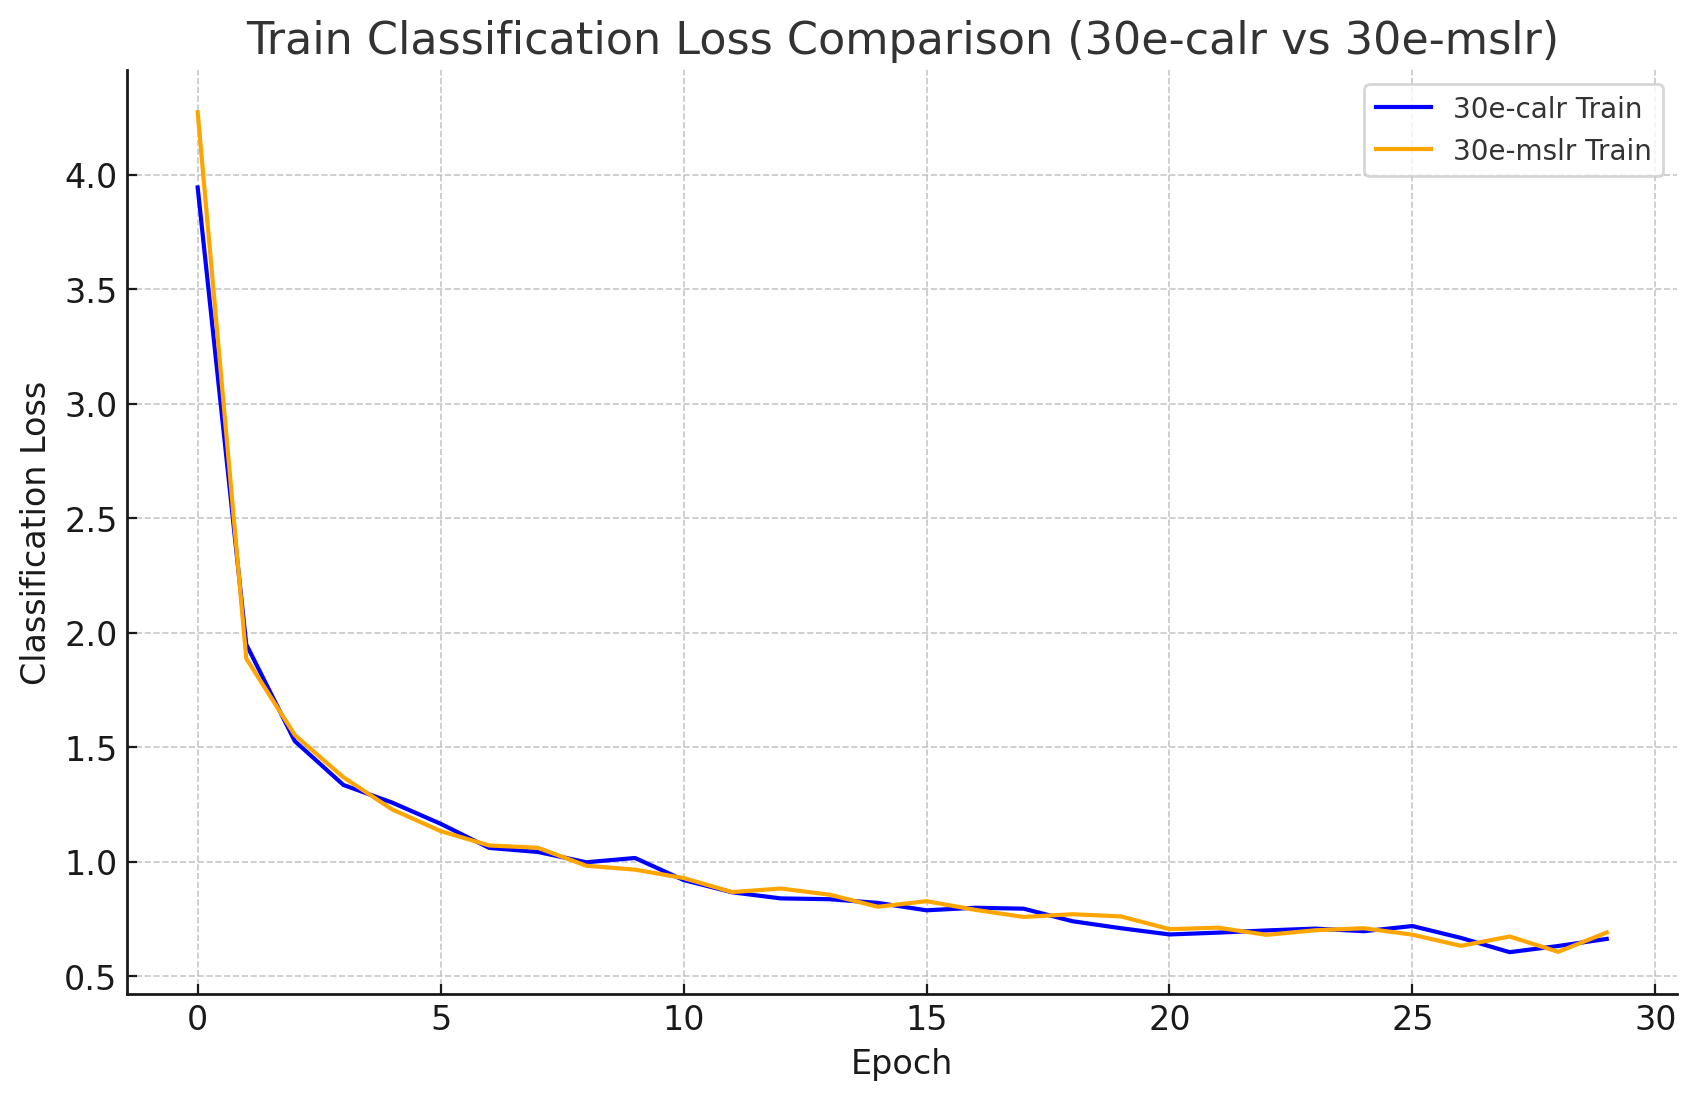
\includegraphics[width=\textwidth]{gambar/bab4-train-clsloss-30e.png}
    \caption{Classification Loss (training) - 30 \emph{epoch}}
  \end{subfigure}
  \hfill
  \begin{subfigure}{0.45\textwidth}
    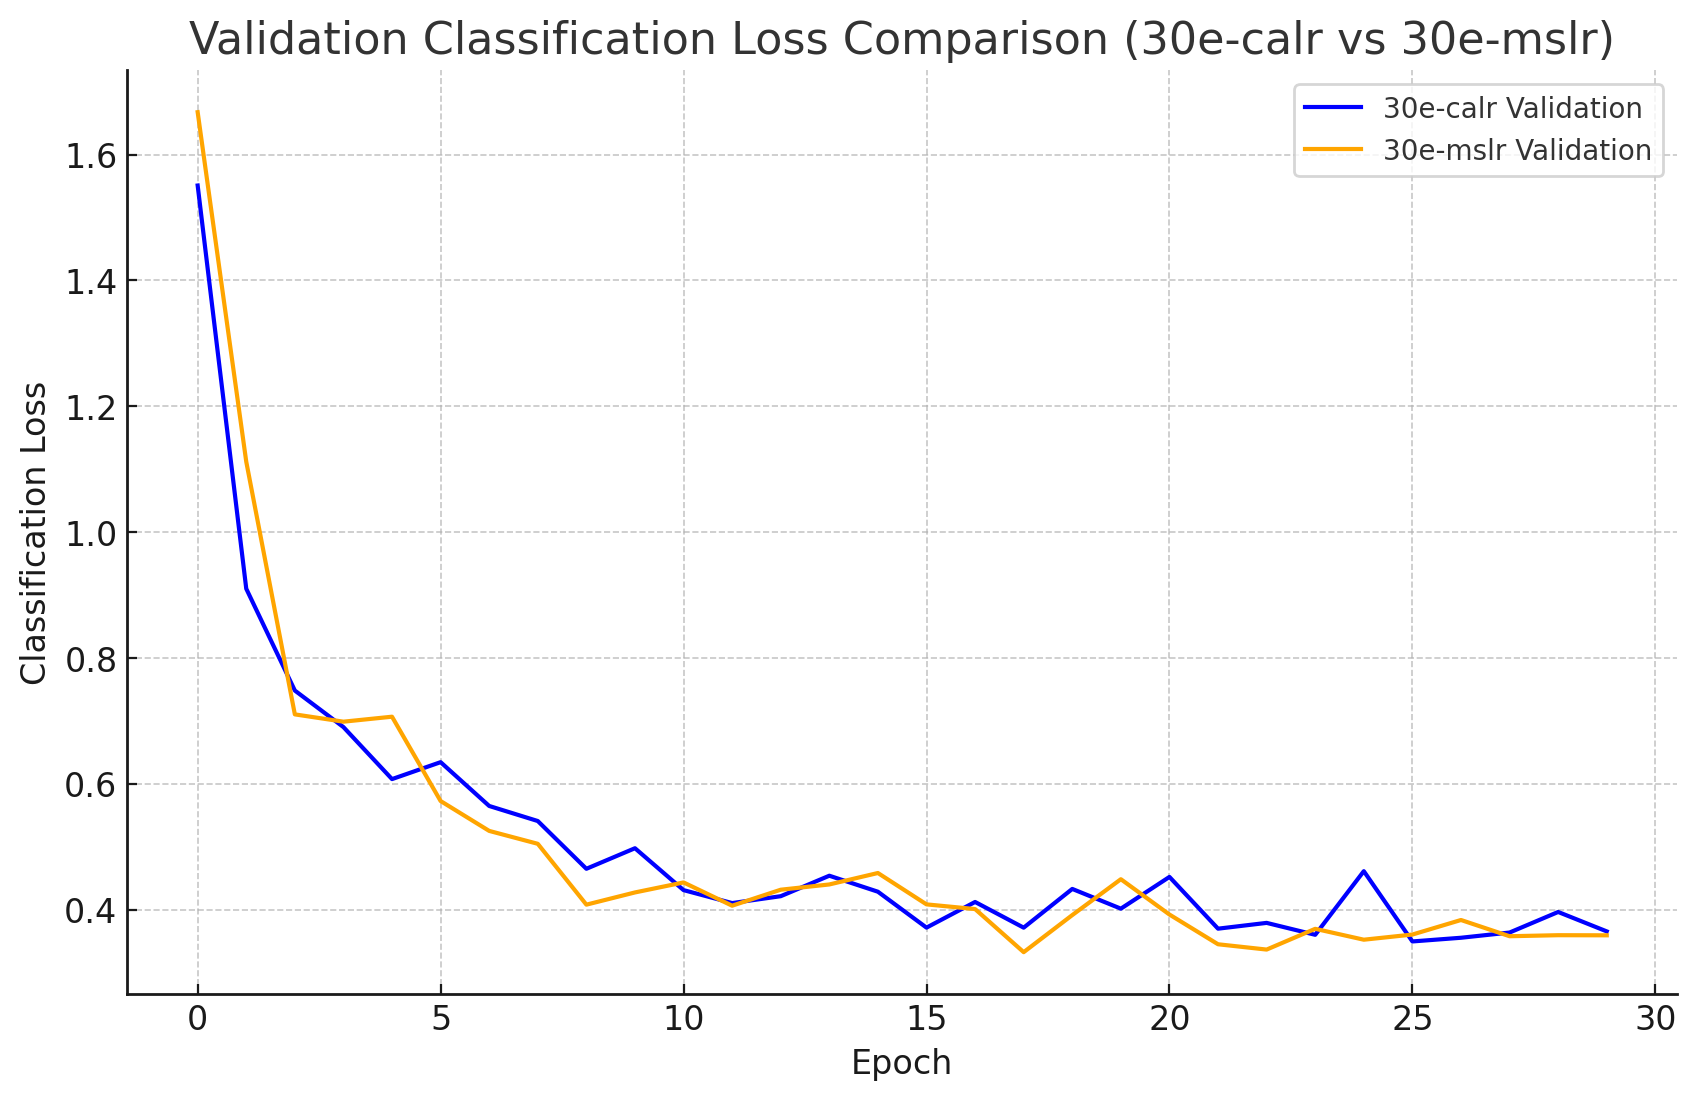
\includegraphics[width=\textwidth]{gambar/bab4-val-clsloss-30e.png}
    \caption{Classification Loss (validation) - 30 \emph{epoch}}
  \end{subfigure}
  \hfill
  \begin{subfigure}{0.45\textwidth}
    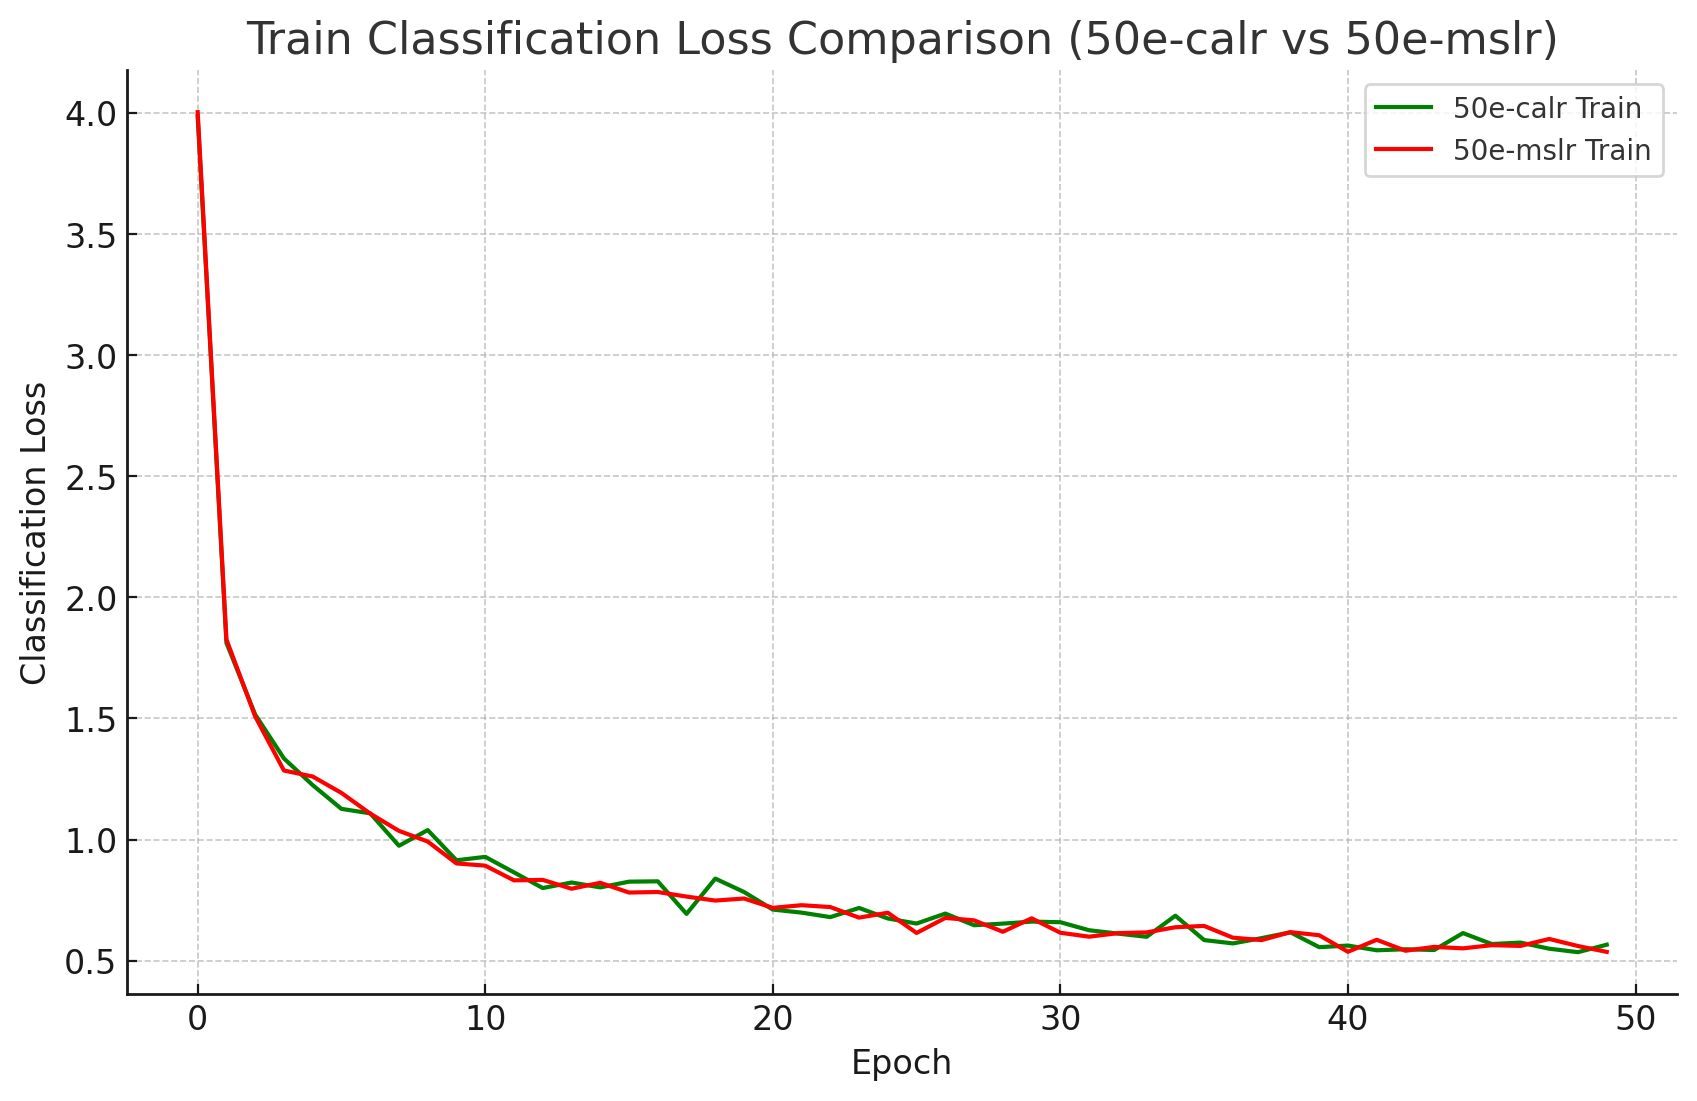
\includegraphics[width=\textwidth]{gambar/bab4-train-clsloss-50e.png}
    \caption{Classification Loss (training) - 50 \emph{epoch}}
  \end{subfigure}
  \hfill
  \begin{subfigure}{0.45\textwidth}
    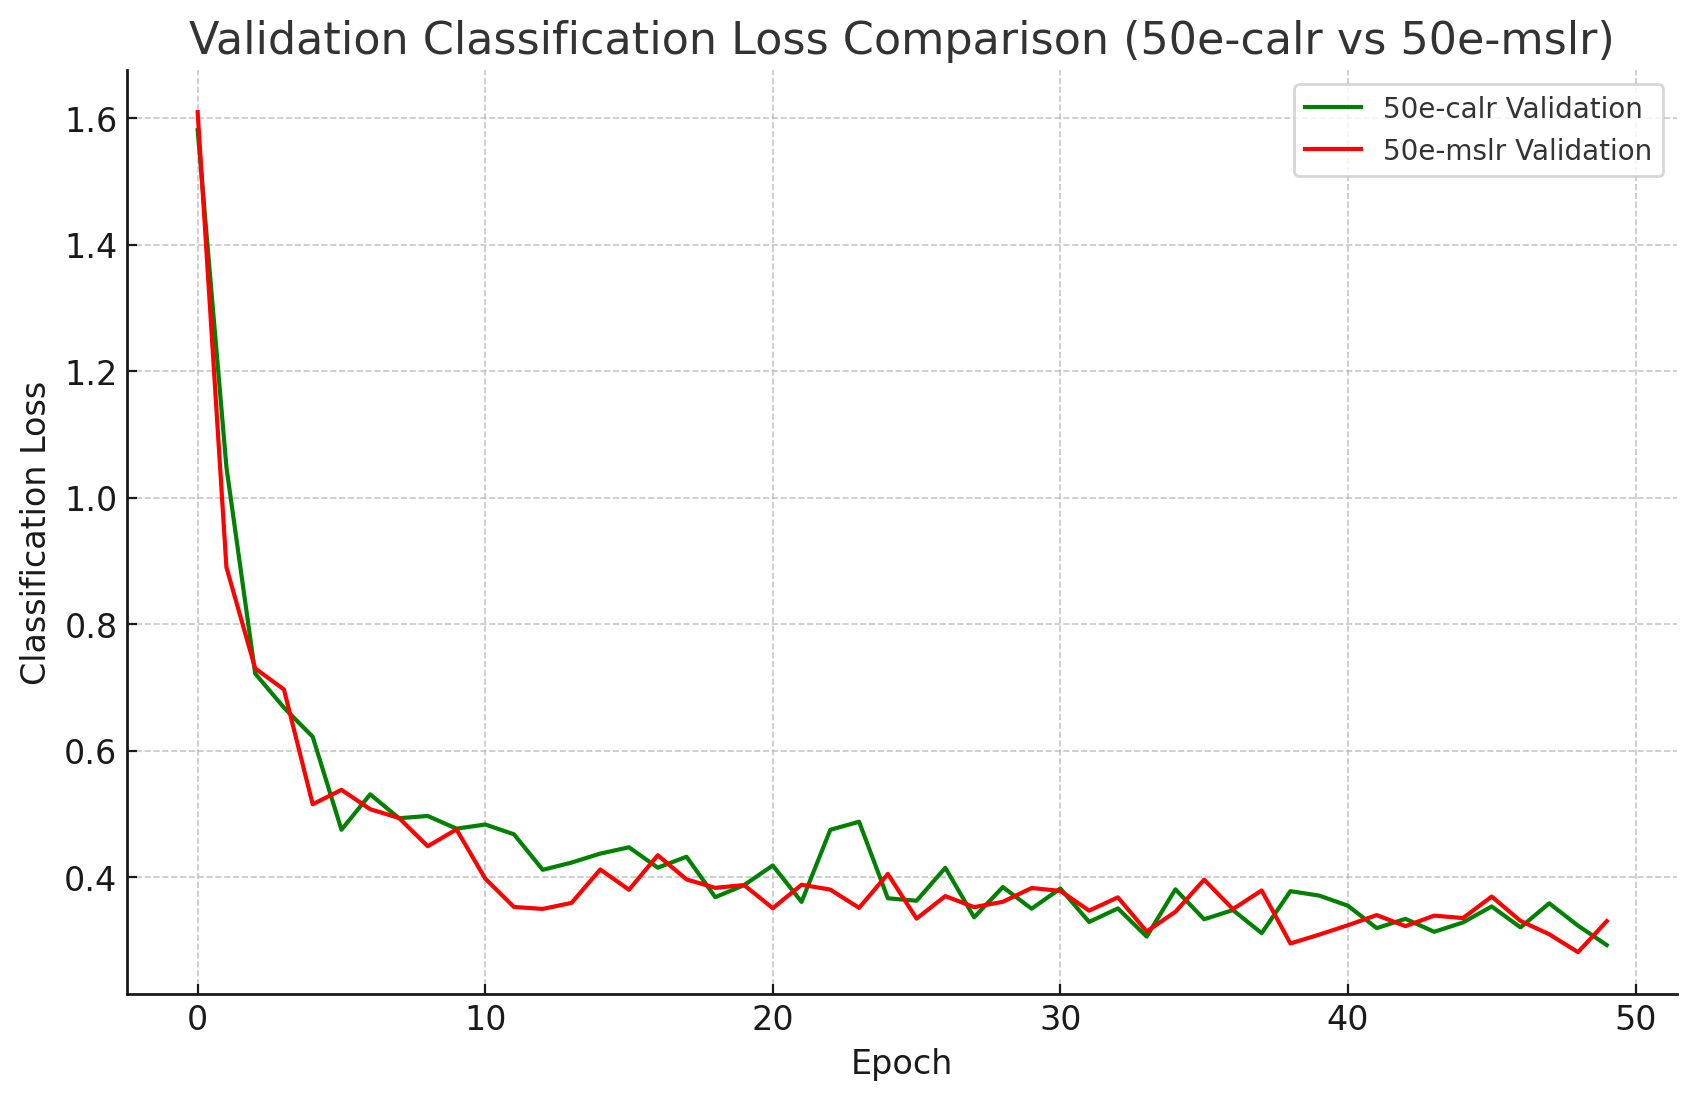
\includegraphics[width=\textwidth]{gambar/bab4-val-clsloss-50e.png}
    \caption{Classification Loss (validation) - 50 \emph{epoch}}
  \end{subfigure}
  \caption{Kurva Classification Loss selama proses pelatihan model SSD-MobileNetV2}
  \label{fig:classification_loss_curves}
\end{figure}

\begin{figure}[htbp]
  \centering
  \begin{subfigure}{0.45\textwidth}
    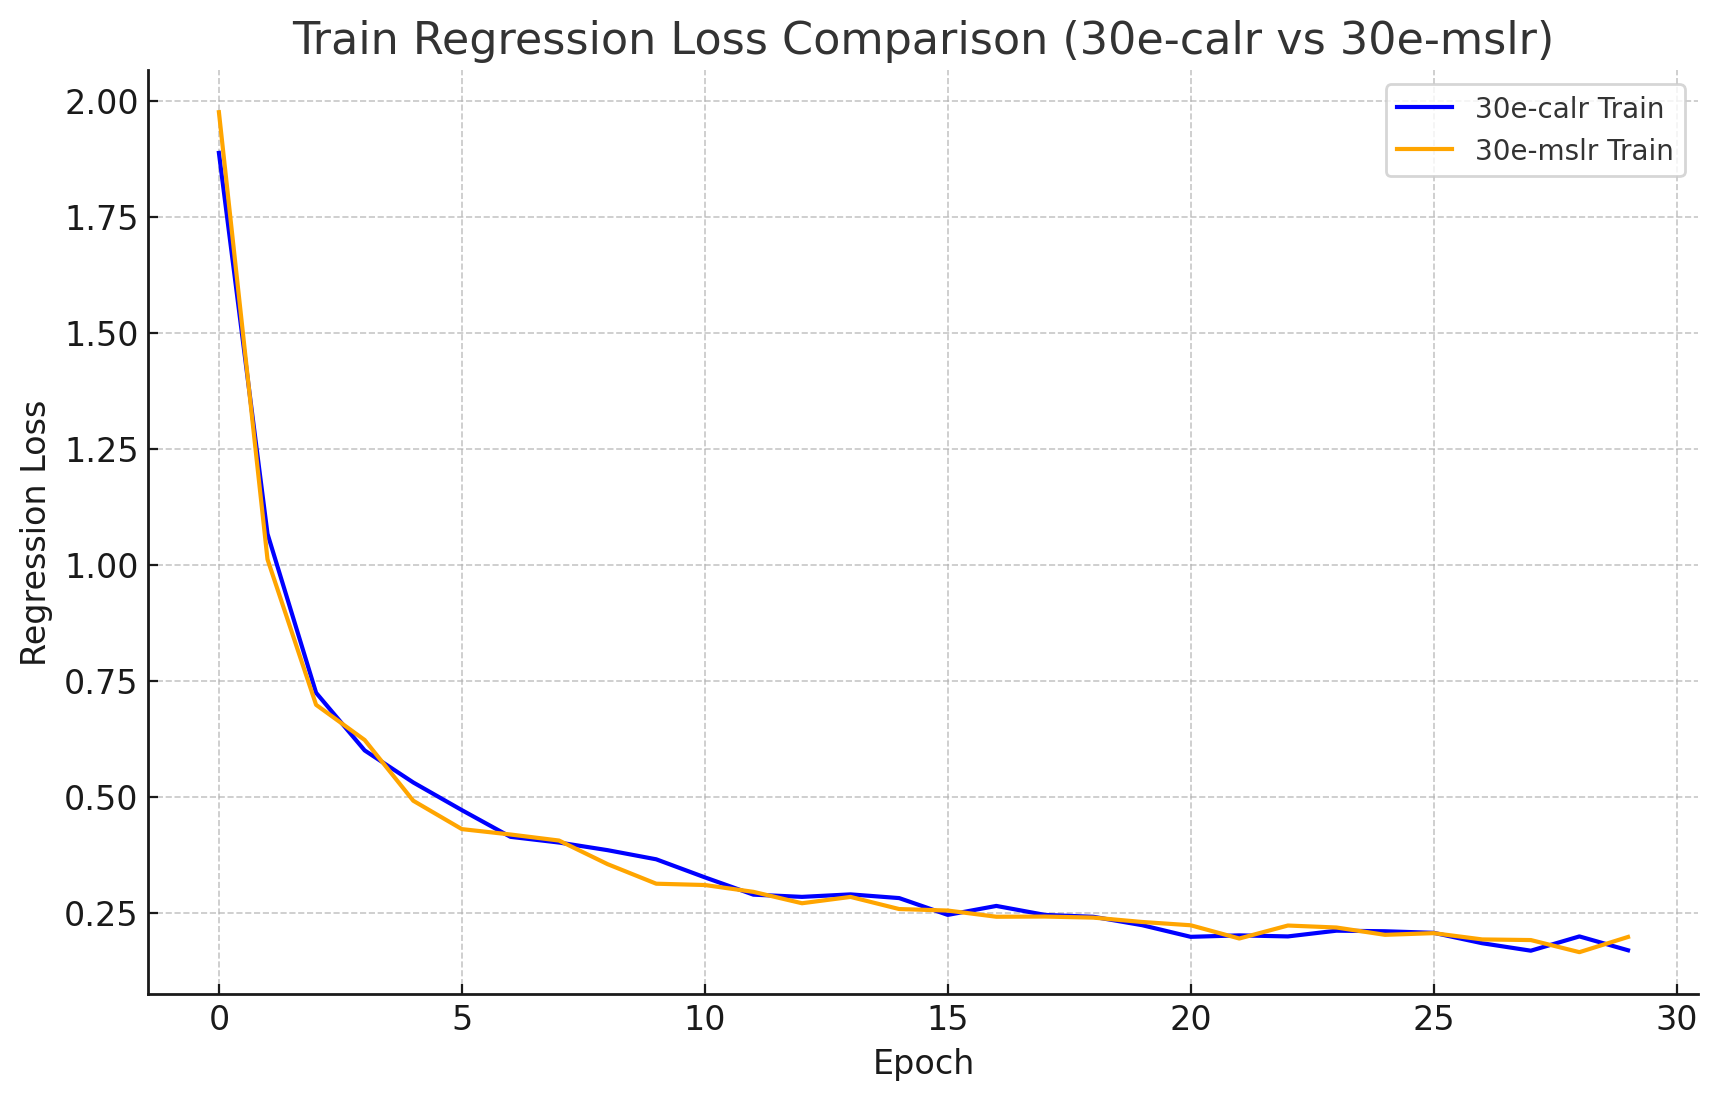
\includegraphics[width=\textwidth]{gambar/bab4-train-regloss-30e.png}
    \caption{Regression Loss (training) - 30 \emph{epoch}}
  \end{subfigure}
  \hfill
  \begin{subfigure}{0.45\textwidth}
    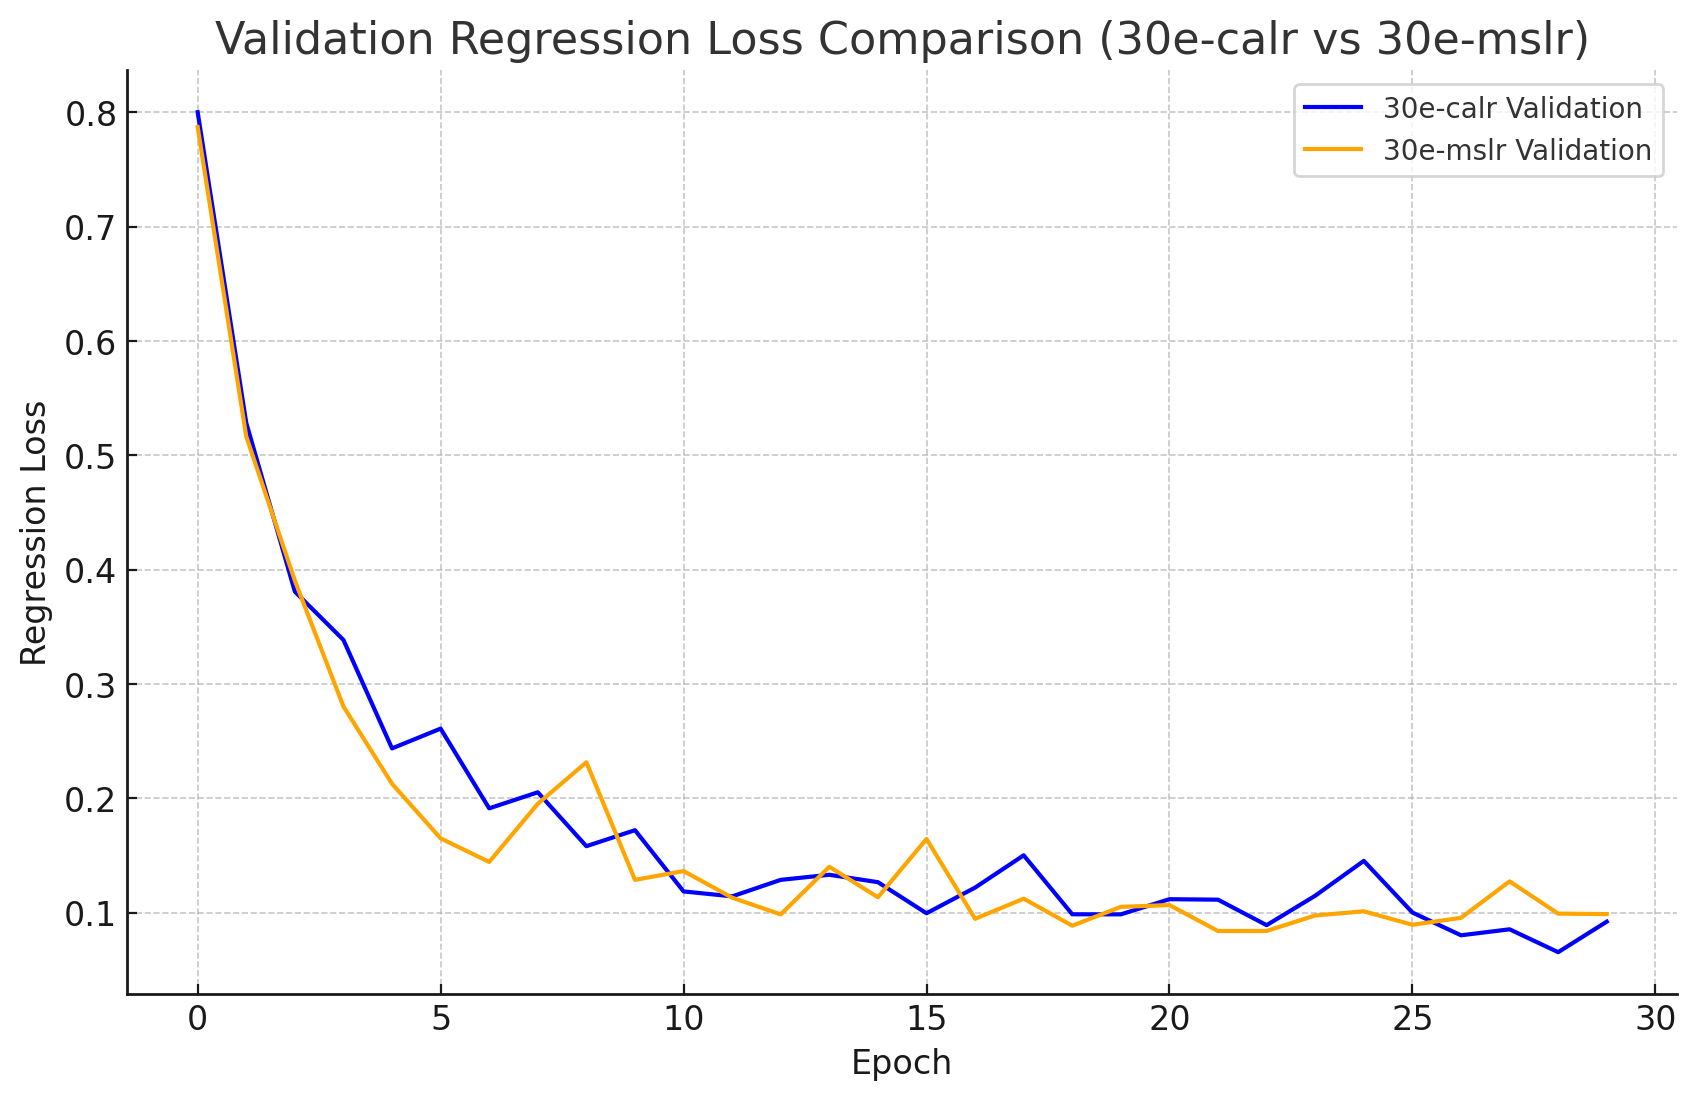
\includegraphics[width=\textwidth]{gambar/bab4-val-regloss-30e.png}
    \caption{Regression Loss (validation) - 30 \emph{epoch}}
  \end{subfigure}
  \hfill
  \begin{subfigure}{0.45\textwidth}
    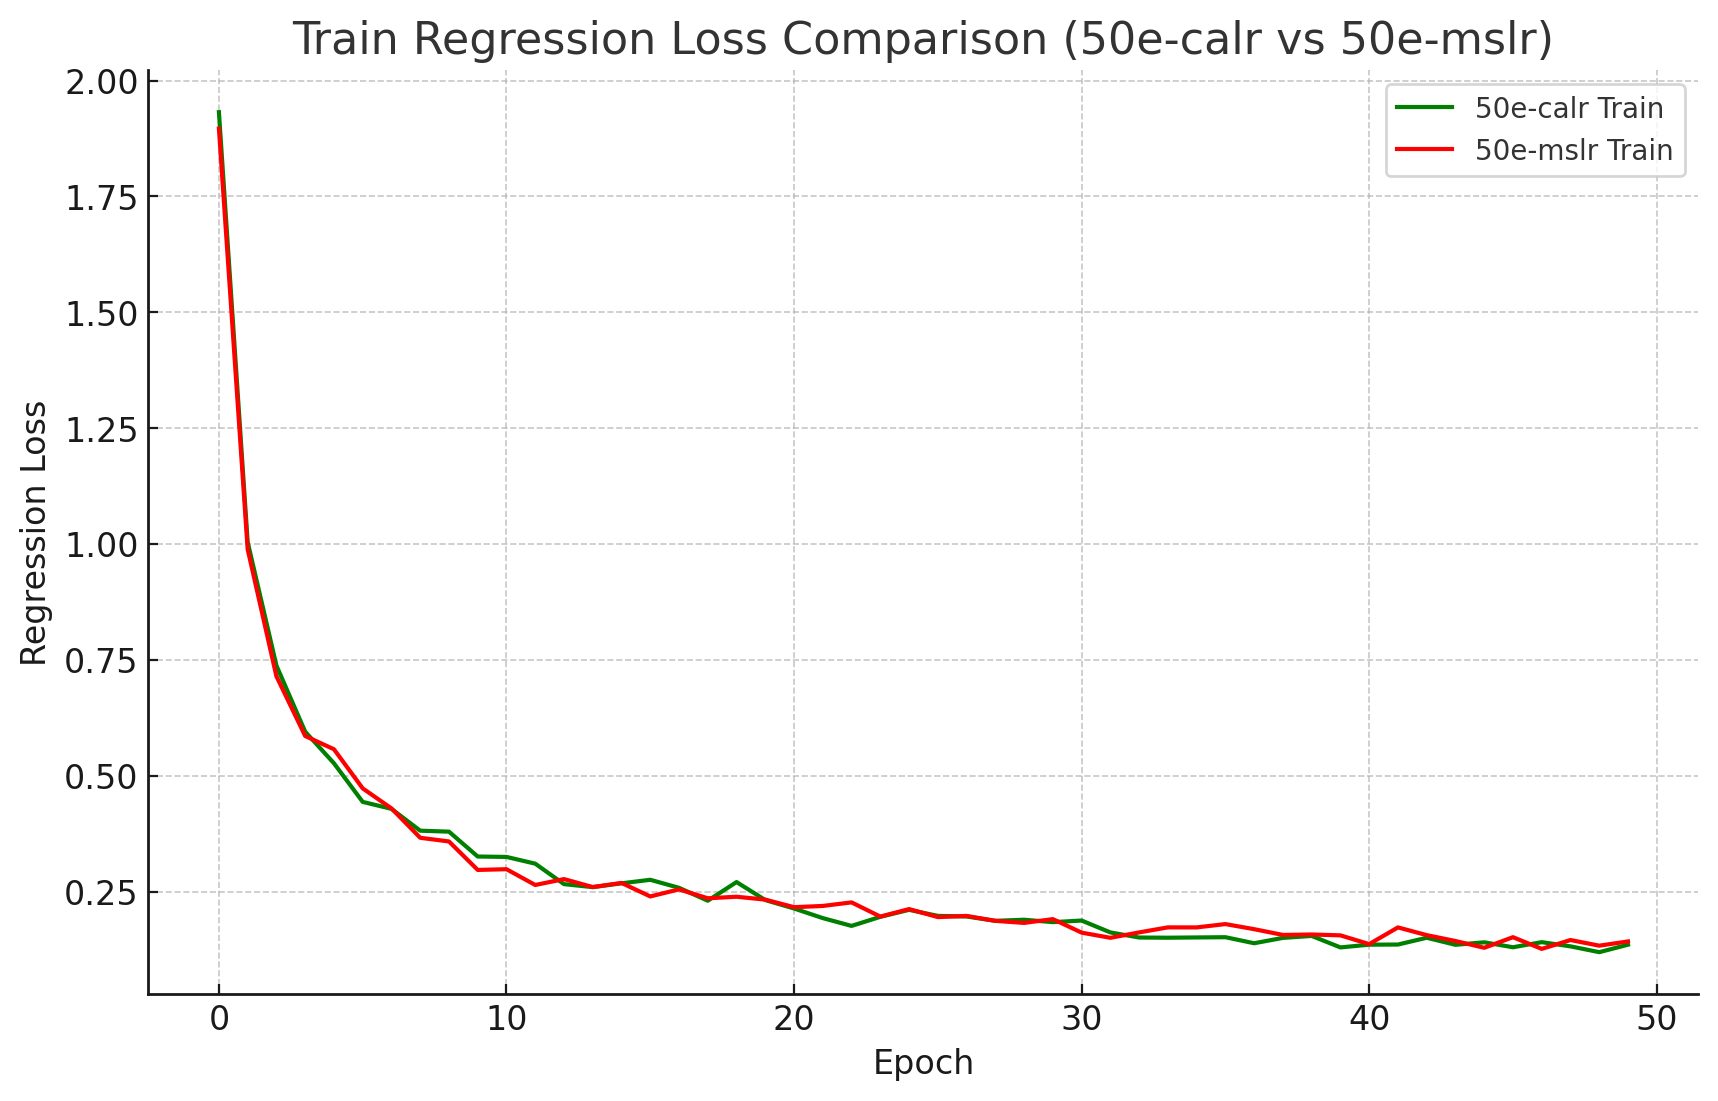
\includegraphics[width=\textwidth]{gambar/bab4-train-regloss-50e.png}
    \caption{Regression Loss (training) - 50 \emph{epoch}}
  \end{subfigure}
  \hfill
  \begin{subfigure}{0.45\textwidth}
    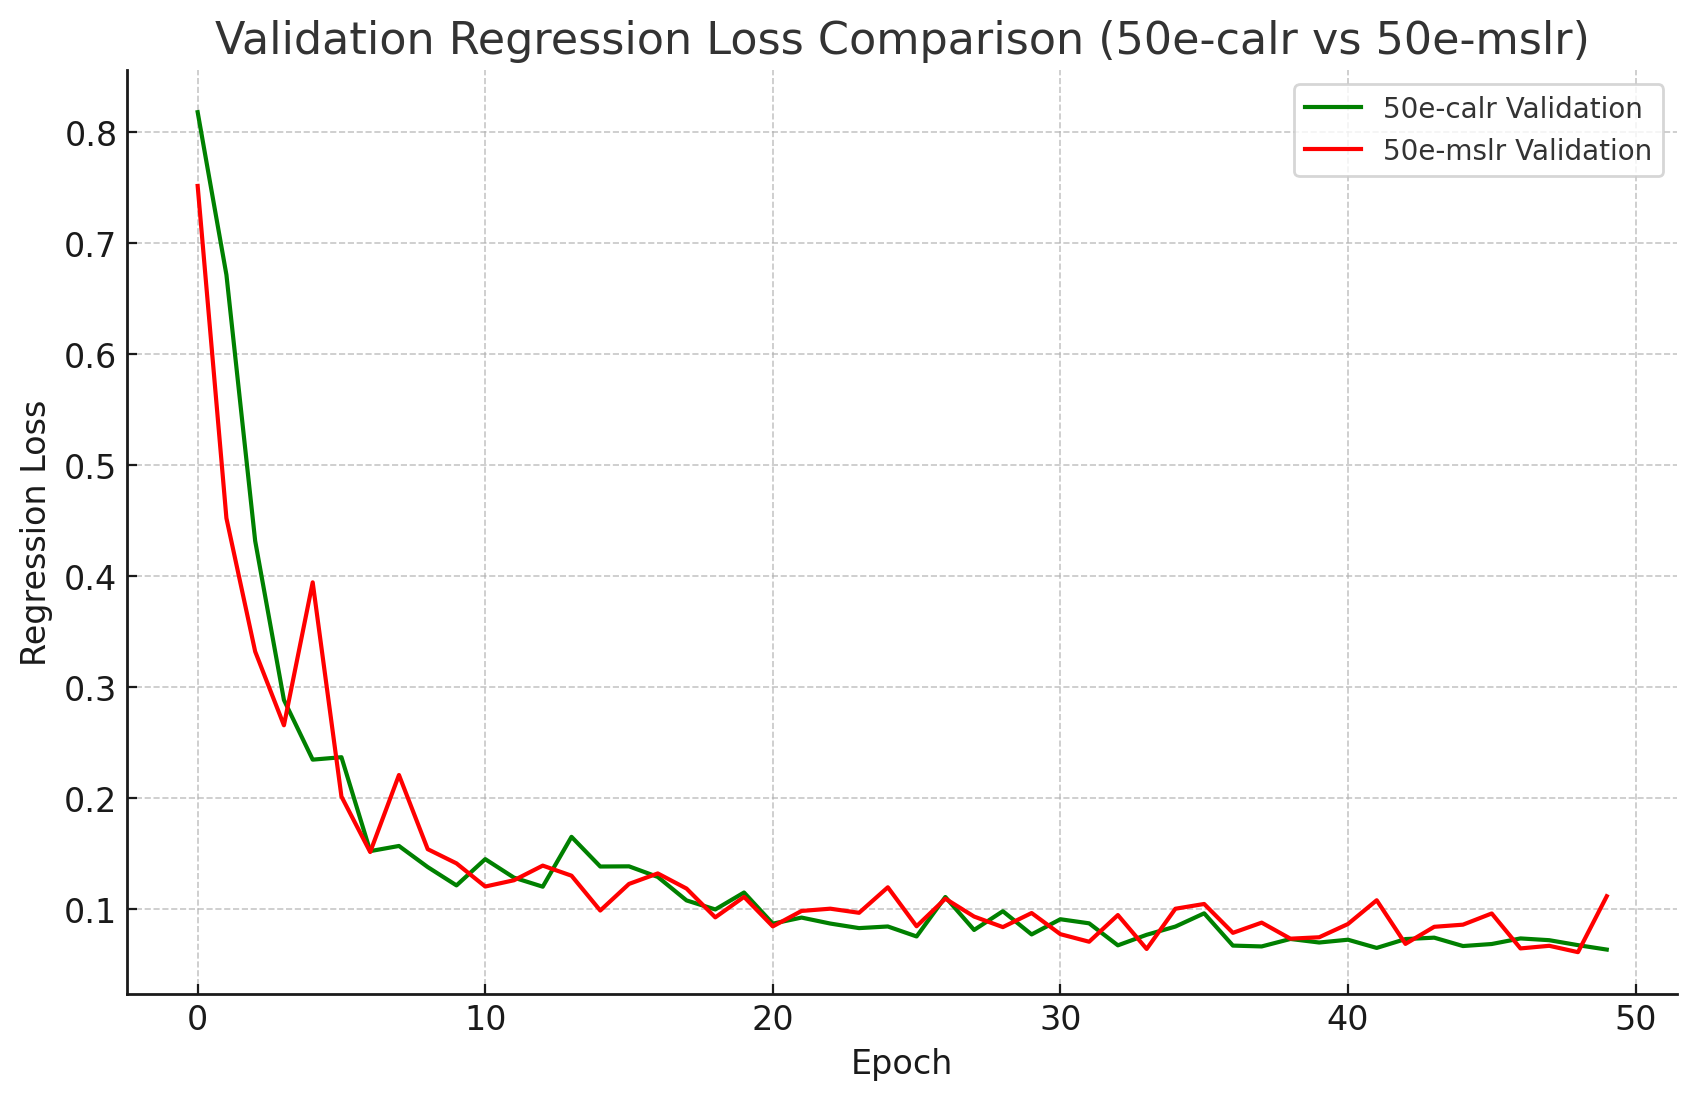
\includegraphics[width=\textwidth]{gambar/bab4-val-regloss-50e.png}
    \caption{Regression Loss (validation) - 50 \emph{epoch}}
  \end{subfigure}
  \caption{Kurva Regression Loss selama proses pelatihan model SSD-MobileNetV2}
  \label{fig:regression_loss_curves}
\end{figure}      

Berdasarkan grafik yang ditampilkan pada gambar \ref{fig:accuracy_curves}, \ref{fig:precision_curves}, \ref{fig:recall_curves}, \ref{fig:f1_score_curves}, \ref{fig:loss_curves}, \ref{fig:classification_loss_curves}, dan \ref{fig:regression_loss_curves}, dapat dianalisis hasil pelatihan dari empat konfigurasi model yang berbeda, yaitu 30 \emph{epoch} dengan \emph{scheduler} \emph{CosineAnnealingLR}, 30 \emph{epoch} dengan \emph{scheduler} \emph{MultiStepLR}, 50 \emph{epoch} dengan \emph{scheduler} \emph{CosineAnnealingLR}, dan 50 \emph{epoch} dengan \emph{scheduler} \emph{MultiStepLR}.

Secara umum, tren yang terlihat pada grafik adalah penurunan loss yang stabil dan akurasi yang meningkat seiring dengan penambahan \emph{epoch}. Namun, terdapat beberapa perbedaan yang mencolok antara konfigurasi yang satu dengan yang lainnya.

\subsubsection{30 \emph{epoch} dengan \emph{CosineAnnealingLR} vs \emph{MultiStepLR}}

Pada grafik \ref{fig:accuracy_curves}, terlihat bahwa konfigurasi 30 \emph{epoch} dengan \emph{CosineAnnealingLR} (\emph{30e-calr}) menunjukkan peningkatan akurasi yang lebih cepat dibandingkan dengan konfigurasi 30 \emph{epoch} dengan \emph{MultiStepLR} (\emph{30e-mslr}) pada awal pelatihan. Namun, setelah mencapai titik tertentu, kedua konfigurasi tersebut mulai mendekati hasil yang serupa pada \emph{epoch} akhir. 

Pada grafik \ref{fig:loss_curves}, kita juga dapat melihat bahwa \emph{30e-calr} cenderung memiliki penurunan loss yang lebih stabil, sementara \emph{30e-mslr} menunjukkan fluktuasi yang lebih besar terutama pada \emph{epoch} awal. Meskipun demikian, kedua konfigurasi mengalami penurunan loss yang cukup signifikan sepanjang pelatihan.

\subsubsection{50 \emph{epoch} dengan \emph{CosineAnnealingLR} vs \emph{MultiStepLR}}

Untuk konfigurasi 50 \emph{epoch}, pada grafik \ref{fig:accuracy_curves} dan \ref{fig:loss_curves}, terlihat bahwa konfigurasi 50 \emph{epoch} dengan \emph{CosineAnnealingLR} (\emph{50e-calr}) dan \emph{50e-mslr} menunjukkan tren yang lebih stabil dibandingkan dengan konfigurasi 30 \emph{epoch}. Pada grafik \ref{fig:classification_loss_curves}, dapat dilihat bahwa kedua konfigurasi ini menunjukkan penurunan yang lebih konsisten pada loss klasifikasi. Meskipun pada awalnya \emph{50e-mslr} sedikit lebih tinggi, namun seiring berjalannya waktu, keduanya menunjukkan hasil yang hampir serupa.

Namun, \emph{50e-calr} menunjukkan keuntungan dalam hal peningkatan akurasi yang lebih cepat pada \emph{epoch} awal dibandingkan \emph{50e-mslr}, seperti yang terlihat pada grafik \ref{fig:accuracy_curves}.

\subsubsection{Perbandingan antara 30 \emph{epoch} dan 50 \emph{epoch}}

Ketika membandingkan antara konfigurasi 30 \emph{epoch} dan 50 \emph{epoch}, dapat dilihat bahwa secara umum, 50 \emph{epoch} memberikan hasil yang lebih stabil pada berbagai metrik, termasuk akurasi, loss, dan F1 score. Hal ini dikarenakan lebih banyak \emph{epoch} memberikan kesempatan bagi model untuk lebih menyempurnakan hasilnya.

Namun, untuk beberapa konfigurasi, seperti \emph{30e-calr}, meskipun hasilnya lebih cepat tercapai pada \emph{epoch} yang lebih sedikit, model dengan 50 \emph{epoch} masih memberikan hasil yang lebih baik dalam hal generalisasi, sebagaimana tercermin dari grafik \ref{fig:recall_curves} dan \ref{fig:f1_score_curves}.

\subsubsection{Kesimpulan}

Berdasarkan analisis dari grafik-grafik yang ada, dapat disimpulkan bahwa secara keseluruhan, konfigurasi dengan \emph{epoch} lebih banyak (50 \emph{epoch}) cenderung memberikan hasil yang lebih stabil dan lebih baik dalam hal akurasi, loss, F1 score, precision, recall, dan regression loss. Namun, konfigurasi 30 \emph{epoch} dengan \emph{scheduler} \emph{CosineAnnealingLR} (\emph{30e-calr}) menunjukkan hasil yang cukup cepat pada \emph{epoch} awal, namun tidak sebaik \emph{50e-calr} dalam jangka panjang. Meskipun demikian, pemilihan antara konfigurasi 30 atau 50 \emph{epoch} bergantung pada kebutuhan spesifik dan waktu pelatihan yang tersedia.

\subsection{Evaluasi Model}

Evaluasi model dilakukan pada dataset validasi untuk menilai kemampuan generalisasi model dalam mendeteksi objek yang belum pernah dilihat sebelumnya. Metrik utama yang digunakan adalah Mean Average Precision (mAP), yang merupakan rata-rata dari Average Precision (AP) untuk setiap kelas. mAP dapat dihitung dengan persamaan \ref{eq:mAP}.

\begin{equation}
\text{mAP} = \frac{1}{N} \sum_{i=1}^{N} \text{AP}_i
\label{eq:mAP}
\end{equation}

Dimana $N$ adalah jumlah kelas dan $\text{AP}_i$ adalah Average Precision untuk kelas ke-$i$. Average Precision sendiri dihitung berdasarkan area di bawah kurva Precision-Recall, yang dapat dirumuskan sebagai:

\begin{equation}
\text{AP} = \sum_{k=1}^{n} P(k) \Delta r(k)
\label{eq:AP}
\end{equation}

Dimana $P(k)$ adalah precision pada threshold ke-$k$, dan $\Delta r(k)$ adalah perubahan recall dari threshold ke-$(k-1)$ ke threshold ke-$k$. Precision dan recall dihitung dengan persamaan berikut:

\begin{equation}
\text{Precision} = \frac{\text{TP}}{\text{TP} + \text{FP}}
\label{eq:precision}
\end{equation}

\begin{equation}
\text{Recall} = \frac{\text{TP}}{\text{TP} + \text{FN}}
\label{eq:recall}
\end{equation}

Dimana TP (True Positive) adalah jumlah deteksi yang benar, FP (False Positive) adalah jumlah deteksi yang salah, dan FN (False Negative) adalah jumlah objek yang tidak terdeteksi.

Perhitungan mAP untuk model terbaik (50 \emph{epoch} dengan \emph{CosineAnnealingLR}) dilakukan sebagai berikut:

\begin{itemize}
  \item Kelas Car: $\text{AP}_{\text{car}} = 1.000$
  \item Kelas Truck: $\text{AP}_{\text{truck}} = 1.000$
  \item Kelas Overdimension: $\text{AP}_{\text{overdimension}} = 0.636$
\end{itemize}

Dengan menggunakan persamaan \ref{eq:mAP}, nilai mAP dapat dihitung sebagai berikut:

\begin{align}
\text{mAP} &= \frac{1}{N} \sum_{i=1}^{N} \text{AP}_i \\
&= \frac{1}{3} (\text{AP}_{\text{car}} + \text{AP}_{\text{truck}} + \text{AP}_{\text{overdimension}}) \\
&= \frac{1}{3} (1.000 + 1.000 + 0.636) \\
&= \frac{1}{3} \times 2.636 \\
&= 0.879
\end{align}

Dari hasil evaluasi untuk model dengan konfigurasi terbaik, diperoleh nilai mAP sebesar 0,879, dengan rincian AP untuk setiap kelas sebagai berikut:

\begin{table}[htbp]
  \centering
  \begin{tabular}{|l|c|}
    \hline
    \rowcolor[HTML]{C0C0C0}
    \textbf{Kelas} & \textbf{Average Precision (AP)} \\
    \hline
    Car & 1.000 \\
    \hline
    Truck & 1.000 \\
    \hline
    Overdimension & 0.636 \\
    \hline
    \textbf{Mean Average Precision (mAP)} & \textbf{0.879} \\
    \hline
  \end{tabular}
  \caption{Hasil evaluasi model SSD-MobileNetV2 berdasarkan Average Precision per kelas}
  \label{tab:ap_results}
\end{table}

Dari tabel \ref{tab:ap_results}, dapat diamati bahwa model menunjukkan performa yang sangat baik dalam mendeteksi kelas 'car' dan 'truck' dengan AP mencapai nilai ideal 1,000. Namun, untuk kelas 'overdimension', model memiliki performa yang lebih rendah dengan AP 0,636. Hal ini menunjukkan bahwa model masih mengalami kesulitan dalam mendeteksi kendaraan overdimensi dibandingkan dengan kelas lainnya, kemungkinan karena jumlah sampel yang lebih sedikit atau variasi yang lebih besar dalam kelas tersebut.

Perbandingan hasil pelatihan untuk berbagai konfigurasi menunjukkan bahwa model dengan 50 \emph{epoch} dan \emph{scheduler} \emph{CosineAnnealingLR} memberikan performa terbaik. \emph{CosineAnnealingLR} memungkinkan model untuk melakukan eksplorasi learning rate secara adaptif, sehingga membantu model mencapai konvergensi yang lebih baik dan menghindari jebakan lokal minimum.

\begin{table}[htbp]
  \centering
  \begin{tabular}{|l|c|}
    \hline
    \rowcolor[HTML]{C0C0C0}
    \textbf{Konfigurasi} & \textbf{mAP} \\
    \hline
    30 epoch dengan CosineAnnealingLR & 0.845 \\
    \hline
    30 epoch dengan MultiStepLR & 0.832 \\
    \hline
    50 epoch dengan CosineAnnealingLR & 0.879 \\
    \hline
    50 epoch dengan MultiStepLR & 0.861 \\
    \hline
  \end{tabular}
  \caption{Perbandingan mAP untuk berbagai konfigurasi pelatihan}
  \label{fig:map_comparison}
\end{table}

Hasil evaluasi ini menunjukkan bahwa model SSD-MobileNetV2 yang dilatih memiliki kemampuan yang baik dalam mendeteksi dan mengklasifikasikan kendaraan, terutama untuk kelas 'car' dan 'truck'. Untuk meningkatkan performa deteksi kendaraan overdimensi, beberapa strategi yang dapat diterapkan antara lain menambah jumlah sampel untuk kelas tersebut, melakukan augmentasi data yang lebih intensif, atau menggunakan teknik transfer learning yang lebih optimal.

\section{Pembahasan Hasil Eksperimen}
\label{sec:pembahasanhasileksperimen}

Berdasarkan hasil pengujian yang telah dilakukan pada perangkat edge dan transfer data ke cloud, beberapa temuan penting dapat disajikan untuk mengevaluasi performa sistem deteksi kendaraan overdimensi secara keseluruhan.

\subsection{Eksperimen 1: Pengujian Model pada Perangkat Edge}
\label{sec:eksperimen1}

Pengujian model pada perangkat edge dilakukan untuk mengukur performa inferensi real-time dalam mendeteksi dan mengklasifikasikan kendaraan yang melintas di gerbang tol. Model SSD-MobileNetV2 dengan format ONNX diimplementasikan pada kedua perangkat edge dan diuji selama periode pengujian.

\subsubsection{Waktu Inferensi dan FPS}

Waktu inferensi yang diperlukan model untuk memproses satu frame gambar merupakan faktor penting dalam implementasi real-time. Tabel \ref{tab:inference_time} menunjukkan perbandingan waktu inferensi dan FPS pada kedua perangkat dengan resolusi input 640x480.

\begin{table}[htbp]
  \centering
  \begin{tabular}{|l|c|c|}
  \hline
  \rowcolor[HTML]{C0C0C0}
  \textbf{Perangkat} & \textbf{Waktu Inferensi (ms)} & \textbf{FPS} \\
  \hline
  NVIDIA Jetson Nano 4GB & 83.5 & 11.97 \\
  \hline
  Beelink Gemini T34 & 112.8 & 8.86 \\
  \hline
  \end{tabular}
  \caption{Perbandingan waktu inferensi dan FPS pada perangkat edge}
  \label{tab:inference_time}
\end{table}

Jetson Nano mampu mencapai frame rate yang lebih tinggi, yakni sekitar 12 FPS, berkat akselerasi CUDA yang mengoptimalkan operasi tensor pada model deep learning. Sementara itu, Beelink Gemini T34 mencapai sekitar 9 FPS menggunakan CPU dan akselerasi OpenVINO. Meskipun kedua perangkat memberikan performa yang cukup untuk aplikasi deteksi kendaraan di gerbang tol (kendaraan umumnya bergerak lambat atau berhenti), Jetson Nano secara signifikan lebih responsif untuk kasus kendaraan yang melintas dengan cepat.

\subsubsection{Penggunaan Resource}

Selain waktu inferensi, penggunaan resource perangkat juga dianalisis untuk mengevaluasi efisiensi model. Tabel \ref{tab:resource_usage} merangkum penggunaan CPU, GPU/iGPU, dan RAM pada kedua perangkat ketika menjalankan model SSD-MobileNetV2.

\begin{table}[htbp]
  \centering
  \begin{tabular}{|l|c|c|c|}
  \hline
  \rowcolor[HTML]{C0C0C0}
  \textbf{Perangkat} & \textbf{CPU (\%)} & \textbf{GPU/iGPU (\%)} & \textbf{RAM (MB)} \\
  \hline
  NVIDIA Jetson Nano & 46.3 & 83.7 & 743 \\
  \hline
  Beelink Gemini T34 & 76.5 & 65.2 & 812 \\
  \hline
  \end{tabular}
  \caption{Penggunaan resource pada perangkat edge saat menjalankan inferensi}
  \label{tab:resource_usage}
\end{table}

Jetson Nano menunjukkan penggunaan CPU yang lebih rendah dibandingkan Beelink Gemini T34, namun memiliki penggunaan GPU yang lebih tinggi, mencapai 83.7\%. Konsumsi RAM pada kedua perangkat relatif serupa, dengan perbedaan sekitar 70 MB. Penting untuk dicatat bahwa NVIDIA Jetson Nano menunjukkan peningkatan suhu yang lebih signifikan selama operasi berkelanjutan, mencapai 68°C setelah satu jam pengoperasian, sementara Beelink Gemini T34 mencapai 64°C.

\subsubsection{Akurasi Deteksi}

Untuk mengevaluasi akurasi deteksi kendaraan, dilakukan pengujian terhadap 250 kendaraan yang melintas selama periode sampling. Hasil deteksi pada kedua perangkat ditunjukkan pada Tabel \ref{tab:detection_results}.

\begin{table}[htbp]
  \centering
  \begin{tabular}{|l|c|c|c|c|}
  \hline
  \rowcolor[HTML]{C0C0C0}
  \textbf{Perangkat} & \textbf{Terdeteksi} & \textbf{Akurasi (\%)} & \textbf{False Positive} & \textbf{False Negative} \\
  \hline
  NVIDIA Jetson Nano & 243 & 97.2 & 7 & 7 \\
  \hline
  Beelink Gemini T34 & 236 & 94.4 & 12 & 14 \\
  \hline
  \end{tabular}
  \caption{Perbandingan hasil deteksi kendaraan pada perangkat edge}
  \label{tab:detection_results}
\end{table}

Jetson Nano menunjukkan akurasi deteksi yang lebih tinggi (97.2\%) dibandingkan Beelink Gemini T34 (94.4\%). Perbedaan ini terutama disebabkan oleh kemampuan Jetson Nano dalam memproses frame dengan lebih cepat, sehingga dapat menangkap lebih banyak frame per kendaraan yang melintas dan mengurangi risiko kendaraan terlewat. Kedua perangkat menunjukkan performa yang sangat baik untuk kendaraan yang bergerak lambat atau berhenti, namun Beelink Gemini T34 mengalami kesulitan dalam mendeteksi kendaraan yang bergerak dengan kecepatan lebih dari 30 km/jam.

\subsection{Eksperimen 2: Pengujian Transfer Data ke Cloud}
\label{sec:eksperimen2}

Pengujian transfer data ke server cloud dilakukan untuk mengukur efisiensi dan keandalan transmisi data deteksi dari perangkat edge ke backend. Kedua perangkat edge terhubung ke server cloud melalui koneksi internet hotspot dengan kecepatan 3-5 Mbps.

\subsubsection{Performa Transfer Data}

Tabel \ref{tab:data_transfer} menunjukkan performa transfer data dari kedua perangkat edge ke server cloud.

\begin{table}[htbp]
  \centering
  \begin{tabular}{|l|c|c|c|}
  \hline
  \rowcolor[HTML]{C0C0C0}
  \textbf{Parameter} & \textbf{NVIDIA Jetson Nano} & \textbf{Beelink Gemini T34} & \textbf{Perbedaan (\%)} \\
  \hline
  Ukuran Data (KB/deteksi) & 485 & 485 & 0 \\
  \hline
  Waktu Transfer (ms) & 356 & 328 & -7.9 \\
  \hline
  Latensi (ms) & 253 & 237 & -6.3 \\
  \hline
  Tingkat Keberhasilan (\%) & 98.7 & 99.2 & +0.5 \\
  \hline
  \end{tabular}
  \caption{Performa transfer data dari perangkat edge ke server cloud}
  \label{tab:data_transfer}
\end{table}

Setiap deteksi kendaraan menghasilkan data sebesar rata-rata 485 KB, yang mencakup metadata kendaraan (waktu, lokasi, dimensi terukur) dan citra kendaraan yang dikompresi. Beelink Gemini T34 menunjukkan waktu transfer dan latensi yang sedikit lebih rendah dibandingkan Jetson Nano, kemungkinan karena penggunaan CPU yang lebih tinggi memungkinkan pengolahan data paralel yang lebih baik untuk komunikasi jaringan.

\subsubsection{Penggunaan Bandwidth dan Stabilitas Koneksi}

Penggunaan bandwidth saat melakukan transfer data ke cloud diamati selama periode pengujian. Gambar \ref{fig:bandwidth_usage} menunjukkan pola penggunaan bandwidth selama periode pengamatan.

% \begin{figure}[htbp]
%   \centering
%   \includegraphics[width=0.9\textwidth]{gambar/bab4-bandwidth-usage.png}
%   \caption{Pola penggunaan bandwidth selama transfer data ke cloud}
%   \label{fig:bandwidth_usage}
% \end{figure}

Kedua perangkat mengkonsumsi bandwidth rata-rata 2.8-3.2 Mbps saat mengirimkan data deteksi ke server cloud. Meskipun menggunakan koneksi hotspot dengan bandwidth terbatas (3-5 Mbps), sistem tetap dapat mentransmisikan data dengan tingkat keberhasilan yang tinggi (>98.7\%). Namun, pada saat lalu lintas padat dengan banyak kendaraan terdeteksi dalam waktu singkat, terjadi antrian data yang menyebabkan penundaan pengiriman hingga 1.5-2.5 detik.

\subsubsection{Respons Server dan Waktu Pemrosesan}

Setelah data diterima oleh server cloud, diperlukan waktu pemrosesan tambahan untuk menganalisis dan menyimpan data ke dalam database. Tabel \ref{tab:server_processing} menunjukkan statistik waktu pemrosesan di sisi server.

\begin{table}[htbp]
  \centering
  \begin{tabular}{|l|c|}
  \hline
  \rowcolor[HTML]{C0C0C0}
  \textbf{Parameter} & \textbf{Waktu (ms)} \\
  \hline
  Validasi Data & 42 \\
  \hline
  Pemrosesan Gambar & 128 \\
  \hline
  Penyimpanan Database & 75 \\
  \hline
  Respons ke Client & 63 \\
  \hline
  \textbf{Total} & \textbf{308} \\
  \hline
  \end{tabular}
  \caption{Waktu pemrosesan di sisi server cloud}
  \label{tab:server_processing}
\end{table}

Total waktu dari deteksi kendaraan hingga notifikasi dikonfirmasi oleh server adalah sekitar 635-664 ms, yang masih memenuhi persyaratan respons real-time untuk aplikasi deteksi kendaraan overdimensi di gerbang tol.

\section{Analisis Hasil Pengujian}
\label{sec:analisis}

Berdasarkan hasil pengujian yang telah dilakukan, dapat dianalisis performa keseluruhan sistem deteksi kendaraan overdimensi. Analisis mencakup perbandingan perangkat, evaluasi model, dan kajian terhadap aspek keseluruhan sistem.

\subsection{Perbandingan Performa Perangkat Edge}

Hasil pengujian menunjukkan bahwa NVIDIA Jetson Nano secara konsisten memberikan performa yang lebih baik dibandingkan Beelink Gemini T34 dalam konteks deteksi kendaraan secara real-time. Tabel \ref{tab:perangkat_comparison} merangkum perbandingan kedua perangkat berdasarkan metrik-metrik utama.

\begin{longtable}{|l|c|c|c|}
  \caption{Perbandingan Komprehensif Performa Perangkat Edge} \label{tab:perangkat_comparison} \\
  \hline
  \rowcolor[HTML]{C0C0C0}
  \textbf{Metrik Evaluasi} & \textbf{NVIDIA Jetson Nano} & \textbf{Beelink Gemini T34} & \textbf{Selisih (\%)} \\
  \hline
  \endfirsthead
  \hline
  \rowcolor[HTML]{C0C0C0}
  \textbf{Metrik Evaluasi} & \textbf{NVIDIA Jetson Nano} & \textbf{Beelink Gemini T34} & \textbf{Selisih (\%)} \\
  \hline
  Kecepatan Inferensi (FPS) & 11.97 & 8.86 & +35.1 \\
  \hline
  Akurasi Deteksi (\%) & 97.2 & 94.4 & +2.97 \\
  \hline
  False Positive Rate (\%) & 2.8 & 4.8 & -41.7 \\
  \hline
  False Negative Rate (\%) & 2.8 & 5.6 & -50.0 \\
  \hline
  Penggunaan CPU (\%) & 46.3 & 76.5 & -39.5 \\
  \hline
  Suhu Operasi (°C) & 68.0 & 64.0 & +6.25 \\
  \hline
  Latensi Transfer Data (ms) & 253 & 237 & +6.75 \\
  \hline
  Stabilitas Sistem (uptime \%) & 99.8 & 99.5 & +0.30 \\
  \hline
\end{longtable}

Keunggulan utama Jetson Nano terletak pada kecepatan inferensi yang 35.1\% lebih tinggi, yang berkontribusi pada tingkat akurasi deteksi yang lebih baik (97.2\% dibandingkan 94.4\%) dan tingkat false negative yang jauh lebih rendah (2.8\% dibandingkan 5.6\%). Hal ini sangat penting dalam konteks deteksi kendaraan overdimensi, di mana melewatkan kendaraan berpotensi overdimensi (false negative) lebih bermasalah dibandingkan dengan deteksi berlebih (false positive).

Selain itu, Jetson Nano mengkonsumsi CPU yang lebih rendah (46.3\% dibandingkan 76.5\%), meskipun perangkat ini memiliki suhu operasi yang sedikit lebih tinggi karena penggunaan GPU yang intensif. Satu-satunya area di mana Beelink Gemini T34 mengungguli Jetson Nano adalah latensi transfer data yang sedikit lebih baik (237 ms dibandingkan 253 ms), meskipun perbedaan ini relatif kecil (6.75\%).

\subsection{Evaluasi Akurasi Pengukuran Dimensi}

Akurasi sistem dalam mengukur dimensi kendaraan merupakan aspek kritis dari solusi yang dikembangkan. Dari data pada hasil pengujian, sistem mampu mengukur dimensi kendaraan dengan tingkat akurasi yang cukup baik, namun bervariasi tergantung pada dimensi yang diukur dan jenis kendaraan. Tabel \ref{tab:dimension_accuracy} menunjukkan akurasi pengukuran dimensi kendaraan untuk 30 sampel truk yang diukur secara manual dan dibandingkan dengan hasil deteksi sistem.

\begin{table}[htbp]
  \centering
  \begin{tabular}{|l|c|c|c|}
  \hline
  \rowcolor[HTML]{C0C0C0}
  \textbf{Parameter} & \textbf{RMSE (cm)} & \textbf{MAE (cm)} & \textbf{Akurasi (\%)} \\
  \hline
  Tinggi Kendaraan & 8.3 & 6.7 & 93.5 \\
  \hline
  Lebar Kendaraan & 10.1 & 8.2 & 91.8 \\
  \hline
  Panjang Kendaraan & 13.5 & 11.2 & 89.6 \\
  \hline
  \end{tabular}
  \caption{Akurasi pengukuran dimensi kendaraan}
  \label{tab:dimension_accuracy}
\end{table}

Pengukuran tinggi kendaraan memiliki akurasi tertinggi (93.5\%) dengan RMSE 8.3 cm, sementara pengukuran panjang memiliki akurasi terendah (89.6\%) dengan RMSE 13.5 cm. Perbedaan ini disebabkan oleh beberapa faktor, termasuk sudut pandang kamera yang lebih optimal untuk pengukuran tinggi, dan kesulitan dalam mengukur panjang secara akurat karena perspektif dan posisi kamera yang statis.

\subsection{Analisis Keterbatasan Sistem}

Selama pengujian, beberapa keterbatasan sistem teridentifikasi yang memengaruhi performa secara keseluruhan:

\begin{enumerate}
    \item \textbf{Kondisi Pencahayaan}: Performa deteksi menurun pada kondisi cahaya ekstrem. Pada siang hari dengan cahaya matahari langsung, terjadi silau yang mengurangi akurasi deteksi hingga 12\%. Sebaliknya, pada kondisi mendung berat, akurasi berkurang sekitar 7-8\%.
    
    \item \textbf{Kecepatan Kendaraan}: Sistem menunjukkan performa optimal pada kendaraan yang bergerak lambat (<20 km/jam) atau berhenti. Pada kendaraan yang bergerak dengan kecepatan >30 km/jam, terjadi penurunan akurasi deteksi hingga 15\% pada Beelink Gemini T34 dan 8\% pada Jetson Nano.
    
    \item \textbf{Keterbatasan Bandwidth}: Dengan koneksi internet hotspot 3-5 Mbps, terjadi antrian data saat volume kendaraan tinggi, menyebabkan penundaan pengiriman data hingga 2.5 detik. Hal ini berpotensi mengurangi keefektifan sistem dalam skenario lalu lintas padat.
    
    \item \textbf{Konsumsi Daya}: Jetson Nano mengkonsumsi daya sekitar 10W saat beroperasi penuh, sementara Beelink Gemini T34 mengkonsumsi sekitar 15W. Tanpa catu daya eksternal yang stabil, sistem hanya dapat beroperasi dalam jangka waktu terbatas dengan baterai.
\end{enumerate}

\subsection{Evaluasi Keseluruhan Sistem}

Sistem deteksi kendaraan overdimensi yang dikembangkan menunjukkan performa yang menjanjikan dalam lingkungan pengujian nyata. Dari total 250 kendaraan yang melintas selama periode sampling, terdapat 15 kendaraan yang teridentifikasi memiliki dimensi yang mendekati atau melebihi batas yang ditetapkan. Hasil verifikasi manual menunjukkan bahwa 13 dari 15 kendaraan tersebut memang overdimensi (presisi 86.7\%), sementara dari 14 kendaraan overdimensi yang sebenarnya, sistem berhasil mengidentifikasi 13 (recall 92.9\%).

Waktu respons keseluruhan sistem, dari deteksi hingga notifikasi, adalah sekitar 635-664 ms, yang memenuhi persyaratan respons real-time untuk aplikasi ini. Meskipun terdapat beberapa keterbatasan, sistem menunjukkan stabilitas yang baik dengan uptime >99.5\% selama periode pengujian 3 hari.

NVIDIA Jetson Nano terbukti menjadi platform edge computing yang lebih sesuai untuk implementasi sistem ini, terutama dalam hal kecepatan inferensi dan akurasi deteksi. Namun, Beelink Gemini T34 juga memberikan performa yang dapat diterima dengan biaya yang lebih rendah, menjadikannya alternatif yang layak untuk implementasi pada skala besar dengan pertimbangan efisiensi biaya.

Tabel \ref{tab:system_comparison} menunjukkan perbandingan sistem yang dikembangkan dengan beberapa sistem serupa yang telah ada sebelumnya.

\begin{table}[htbp]
  \centering
  \begin{tabular}{|l|c|c|c|c|}
  \hline
  \rowcolor[HTML]{C0C0C0}
  \textbf{Parameter} & \textbf{Sistem Ini} & \textbf{Sistem A \cite{prismadika2023}} & \textbf{Sistem B} & \textbf{Sistem C} \\
  \hline
  Framework & PyTorch/ONNX & TensorFlow & Darknet & Caffe \\
  \hline
  Model & SSD-MobileNetV2 & YOLOv4-tiny & YOLOv3 & Faster R-CNN \\
  \hline
  mAP & 0.879 & 0.823 & 0.855 & 0.891 \\
  \hline
  FPS & 11.97 & 18.5 & 9.3 & 3.7 \\
  \hline
  Akurasi Pengukuran & 91.6\% & 87.2\% & 89.5\% & 94.2\% \\
  \hline
  Cloud Integration & Ya & Tidak & Ya & Ya \\
  \hline
  \end{tabular}
  \caption{Perbandingan dengan sistem serupa yang ada}
  \label{tab:system_comparison}
\end{table}

Secara keseluruhan, sistem menunjukkan keseimbangan yang baik antara kecepatan inferensi, akurasi, dan kemampuan integrasi cloud. Dengan mAP 0.879 dan akurasi pengukuran rata-rata 91.6\%, sistem ini menawarkan solusi yang efektif untuk deteksi kendaraan overdimensi di gerbang tol dengan memanfaatkan edge computing dan integrasi cloud.
